\section{Results}
\label{sec:Results}

%%%%%%%%%%%%%%%%%%%%%%%
%4.Experimental Results (show the most relevant results to illustrate the merits and the possible unresoved issues)
%%%%%%%%%%%%%%%%%%%%%%%

To evaluate the implemented EKF a testing environment with a pre-defined trajectory was created. The robot would drive one rectangular shaped lap in one part of the pre-acquired map. In figure \ref{fig:test_map} the map is shown. 
Both, the odometry states and the EKF estimated stated plus their covariance, were saved in order to compare them afterwards.

The test results are shown in figure \ref{fig:ekf_odom} with the covariance ellipses being calculated as 95\,\% confidence ellipses. 
With only the odometry measuring the current robot state, the calculated position after one lap, is about 15\,cm away from the starting point. Due to poor odometry calibration, sensor errors or wheel slippage, the odometry accumulates a lot of errors during this short distance.
\begin{figure}[h]
\centering
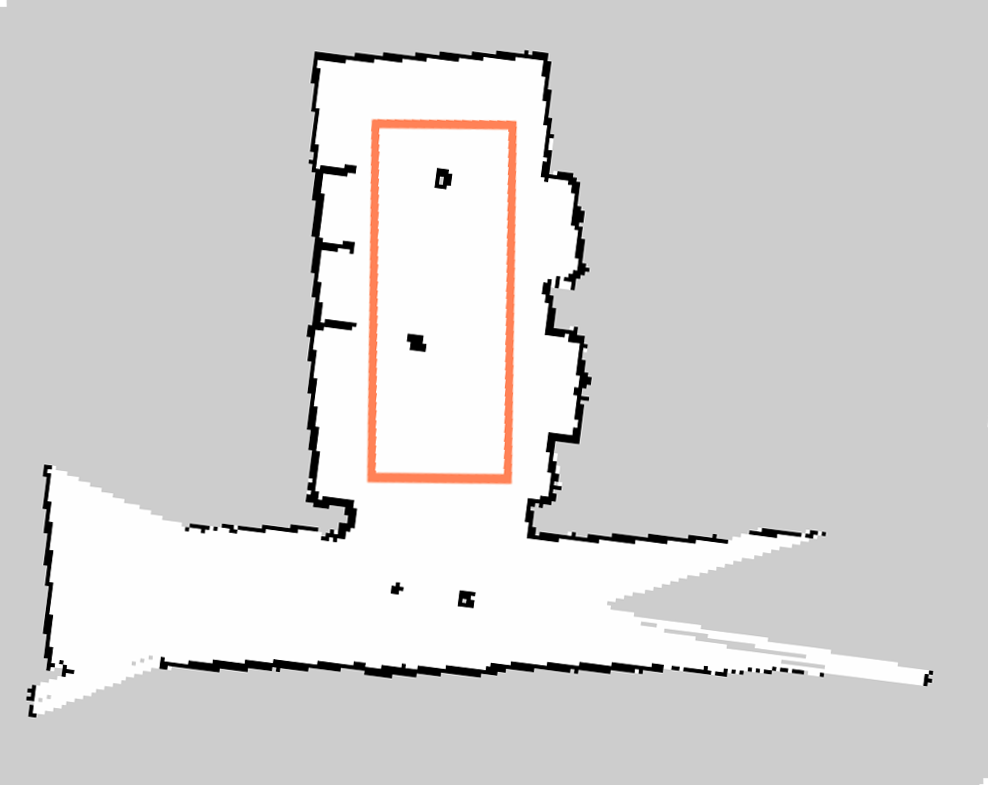
\includegraphics[width=0.4\textwidth]{figures/test_map}
      \caption{Used map and trajectory for testing}
      \label{fig:test_map}
\end{figure}

The EKF predicted states stay much closer to the real trajectory. Every time the ICP is able to match the predicted and the real point cloud the accumulated errors are corrected by a laser based update. Some of these corrections can be recognised as a small jump of the EKF state in figure \ref{fig:ekf_odom}. Due to the modelled motion model with its noise matrix $Q$, the covariance grows during the times, where there are no matches. It then decreases heavily with a successful match. Therefore, the shown covariance ellipses are smaller after a jump in the state. The left part of the trajectory in  figure \ref{fig:ekf_odom} shows this process. Especially as the shape of odometry only and EKF are identical. The EKF only relies on odometry information at this part, before it is able to recover with a laser based update. In the end the EKF predicted state is only about 2.5\,cm away from the actual starting position. 


For obtaining the map displayed in figure \ref{fig:test_map} and evaluating the EKF's performance, some extra obstacles were placed in the environment. Although the implemented EKF was able to converge without these obstacles, the provided extra information by these reference objects improved its performance. Especially in the lower part of the map, with the two sideways being out of range of the laser rangefinder, the obstacles helped the EKF to match successfully.

During the testing of the system, the environment was not static. The environment consisted in an elevator room where  people were walking around and doors were opened and closed. Although this was not the ideal environment, it was noticed that it did not affect the behaviour of the EKF algorithm at all. The EKF algorithm was able to remain stable in terms of position estimate and did not diverge, even though the pre-acquired map was not perfectly matching with the real world. Obviously this robustness to a dynamic environment will diminish with an increasing amount of dynamic changes to the environment.
\begin{figure}
	\centering
	\newlength\figureheight 
	\newlength\figurewidth 
	\setlength\figureheight{10cm} 
	\setlength\figurewidth{5cm}
	% This file was created by matlab2tikz.
%
%The latest updates can be retrieved from
%  http://www.mathworks.com/matlabcentral/fileexchange/22022-matlab2tikz-matlab2tikz
%where you can also make suggestions and rate matlab2tikz.
%
\definecolor{mycolor1}{rgb}{0.00000,0.44700,0.74100}%
\definecolor{mycolor2}{rgb}{0.85000,0.32500,0.09800}%
%
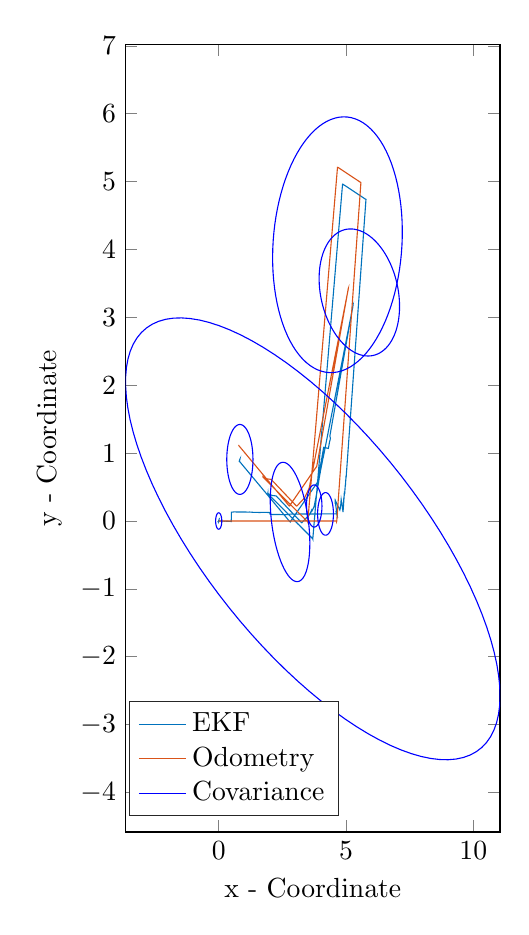
\begin{tikzpicture}

\begin{axis}[%
width=0.951\figurewidth,
height=\figureheight,
at={(0\figurewidth,0\figureheight)},
scale only axis,
xmin=-3.65567043160841,
xmax=11.0503692930476,
xlabel={x - Coordinate},
ymin=-4.5810705877836,
ymax=7.01772525956604,
ylabel={y - Coordinate},
axis background/.style={fill=white},
%title style={font=\bfseries},
%title={Comaprison EKF vs. Odometry},
legend style={at={(0.01,0.02)},anchor=south west,legend cell align=left,align=left,draw=white!15!black}
]
\addplot [color=mycolor1,solid]
  table[row sep=crcr]{%
0	0\\
-8.99303e-06	-5.40527e-05\\
2.17086e-05	-2.51734e-06\\
-2.24523e-06	-1.70597e-05\\
-4.25144e-05	-8.63842e-06\\
-1.31562e-05	2.37659e-05\\
-5.58612e-05	-3.81668e-05\\
-4.92433e-05	-4.6934e-05\\
-2.96289e-05	-9.53623e-05\\
-2.66108e-05	-0.000232664\\
-4.47759e-05	-0.000507632\\
-9.0954e-05	-0.000225401\\
-3.57867e-05	-0.0001007\\
-1.98518e-05	0.000211849\\
-0.000122833	0.000239343\\
-0.000537376	6.70162e-05\\
-0.000684625	4.86359e-05\\
-0.00022773	0.000493194\\
-0.000715586	9.63836e-05\\
-0.000794078	-7.32837e-06\\
-0.000794242	-7.43474e-05\\
-0.000819937	-0.000171553\\
-0.000846709	-4.88608e-05\\
-0.000860822	-5.96617e-05\\
-0.000933668	-0.00022071\\
-0.000980399	-0.000210013\\
-0.000952743	-9.91084e-05\\
-0.000905564	7.99016e-05\\
-0.000940711	0.000136672\\
-0.000911315	8.06237e-05\\
-0.000931877	0.000139363\\
-0.00101525	0.000336452\\
-0.00105081	0.000287735\\
-0.00108643	0.000238942\\
-0.00118176	0.00044612\\
-0.00120185	0.000748023\\
-0.00125853	0.000693474\\
-0.00128901	0.000609358\\
-0.0013596	0.000719122\\
-0.00142448	0.000874837\\
-0.00149413	0.000885566\\
-0.00151513	0.00082243\\
-0.00153613	0.000759267\\
-0.0016636	0.000803136\\
-0.00247203	-1.28329e-05\\
-0.00255544	0.000292097\\
-0.0024764	2.79823e-05\\
-0.00247305	6.38879e-05\\
-0.00246969	9.98e-05\\
-0.00237186	0.000370163\\
-0.00252749	0.000404891\\
-0.00249267	0.000735529\\
-0.00271175	0.00102174\\
-0.00331469	0.000831659\\
-0.0033643	0.000806412\\
-0.00299684	0.000870855\\
0.000923549	0.000846972\\
0.000923549	0.000846972\\
0.00692355	0.000846972\\
0.0129235	0.000846972\\
0.0177545	0.000842145\\
0.0225796	0.000377953\\
0.0285796	0.000377953\\
0.0344753	0.000228742\\
0.0392058	-0.000149949\\
0.0441305	-0.000189501\\
0.0501937	-0.000440683\\
0.0551844	-0.000651284\\
0.0611225	-0.000683229\\
0.0660048	-0.000627163\\
0.0718839	-0.000686771\\
0.0768828	-0.000920045\\
0.0828055	-0.000874538\\
0.0997483	-0.00103746\\
0.0995645	-0.000934072\\
0.0993817	-0.000831733\\
0.1062	-0.000730294\\
0.112713	-0.00120775\\
0.120109	-0.0017081\\
0.126081	-0.00169386\\
0.132955	-0.00200364\\
0.139862	-0.00192081\\
0.14592	-0.00207596\\
0.152907	-0.00213684\\
0.159007	-0.00241566\\
0.165899	-0.00252266\\
0.173085	-0.00268394\\
0.178636	-0.00269227\\
0.185665	-0.0024271\\
0.191762	-0.00264615\\
0.198284	-0.00236261\\
0.205339	-0.00249046\\
0.211421	-0.0028206\\
0.21834	-0.00256004\\
0.224242	-0.00266586\\
0.231201	-0.00279169\\
0.238004	-0.00288286\\
0.243954	-0.00252526\\
0.250936	-0.00251561\\
0.27089	-0.00255836\\
0.270697	-0.00258892\\
0.276505	-0.0026195\\
0.283365	-0.00246498\\
0.296312	-0.00325832\\
0.296211	-0.00386181\\
0.303109	-0.00446297\\
0.309109	-0.00446297\\
0.316212	-0.00464715\\
0.322054	-0.00480169\\
0.329054	-0.00480169\\
0.334938	-0.00473121\\
0.342044	-0.0048943\\
0.34913	-0.00495963\\
0.354754	-0.00494893\\
0.361754	-0.00494893\\
0.368832	-0.00562896\\
0.375602	-0.00529554\\
0.383496	-0.00539269\\
0.390496	-0.00539269\\
0.399496	-0.00539269\\
0.407552	-0.00491779\\
0.414445	-0.00486865\\
0.423392	-0.00504498\\
0.431524	-0.00578282\\
0.437865	-0.00510465\\
0.446659	-0.00535096\\
0.45355	-0.00639202\\
0.46155	-0.00639202\\
0.470468	-0.00680558\\
0.477377	-0.00683064\\
0.485377	-0.00683064\\
0.493554	-0.00703389\\
0.49877	0.130634\\
0.50666	0.130602\\
0.51452	0.130874\\
0.52252	0.130874\\
0.530533	0.131146\\
0.538311	0.131255\\
0.546311	0.131255\\
0.554324	0.13121\\
0.563496	0.132231\\
0.571496	0.132231\\
0.57968	0.132324\\
0.589888	0.133931\\
0.597888	0.133931\\
0.605888	0.133931\\
0.613868	0.134165\\
0.621868	0.134165\\
0.629865	0.134139\\
0.637869	0.134391\\
0.645839	0.134418\\
0.653884	0.134506\\
0.660582	0.133887\\
0.668735	0.134004\\
0.675579	0.13309\\
0.683579	0.13309\\
0.691579	0.13309\\
0.779185	0.13271\\
0.779244	0.132528\\
0.787302	0.132352\\
0.795303	0.132352\\
0.803466	0.132103\\
0.812466	0.132103\\
0.821457	0.132316\\
0.830457	0.132316\\
0.839538	0.13232\\
0.849538	0.13232\\
0.858557	0.132209\\
0.868557	0.132209\\
0.878606	0.131988\\
0.888606	0.131988\\
0.897607	0.132039\\
0.907543	0.132199\\
0.917543	0.132199\\
0.926603	0.132051\\
0.936603	0.132051\\
0.945659	0.131859\\
0.955659	0.131859\\
0.965735	0.132091\\
0.975735	0.132091\\
0.984866	0.132231\\
0.994866	0.132231\\
1.005	0.132101\\
1.02394	0.13273\\
1.02394	0.13273\\
1.04299	0.132242\\
1.04299	0.132242\\
1.06298	0.132382\\
1.06298	0.132382\\
1.07206	0.132067\\
1.08206	0.132067\\
1.10224	0.131386\\
1.10224	0.131386\\
1.11133	0.131564\\
1.12133	0.131564\\
1.13146	0.131556\\
1.14046	0.131556\\
1.15049	0.131469\\
1.16049	0.131469\\
1.16951	0.131544\\
1.17954	0.131618\\
1.18963	0.1317\\
1.19963	0.1317\\
1.20863	0.131982\\
1.21863	0.131982\\
1.22884	0.131755\\
1.23784	0.131755\\
1.25802	0.130127\\
1.25802	0.130127\\
1.26695	0.129961\\
1.27695	0.129961\\
1.28695	0.129977\\
1.29697	0.129913\\
1.30668	0.128732\\
1.31668	0.128732\\
1.32673	0.128651\\
1.33621	0.128125\\
1.34621	0.128125\\
1.3562	0.128001\\
1.3652	0.128001\\
1.37526	0.127794\\
1.38526	0.127794\\
1.39422	0.127796\\
1.40426	0.127606\\
1.41426	0.127606\\
1.4243	0.12753\\
1.4333	0.12753\\
1.45348	0.126801\\
1.45348	0.126801\\
1.46249	0.126617\\
1.47249	0.126617\\
1.48252	0.12638\\
1.49152	0.12638\\
1.50155	0.126354\\
1.51155	0.126354\\
1.52151	0.126311\\
1.53051	0.126311\\
1.5407	0.12607\\
1.5507	0.12607\\
1.55969	0.126013\\
1.56969	0.126013\\
1.57972	0.125926\\
1.58872	0.125926\\
1.59872	0.125926\\
1.60871	0.125564\\
1.61771	0.125564\\
1.62765	0.125485\\
1.63765	0.125485\\
1.64856	0.126664\\
1.65756	0.126664\\
1.66791	0.126534\\
1.67791	0.126534\\
1.68691	0.126534\\
1.69691	0.126534\\
1.70691	0.126534\\
1.71591	0.126534\\
1.72599	0.126211\\
1.73599	0.126211\\
1.74599	0.126211\\
1.75499	0.126211\\
1.76492	0.1261\\
1.77492	0.1261\\
1.78392	0.1261\\
1.79392	0.1261\\
1.80392	0.1261\\
1.81292	0.1261\\
1.82292	0.1261\\
1.83292	0.1261\\
1.84192	0.1261\\
1.85192	0.1261\\
1.86192	0.1261\\
1.87192	0.1261\\
1.88092	0.1261\\
1.89092	0.1261\\
1.90092	0.1261\\
1.90992	0.1261\\
1.92053	0.125904\\
1.93053	0.125904\\
1.93953	0.125904\\
1.94953	0.125904\\
1.95953	0.125904\\
1.96853	0.125904\\
1.97834	0.124713\\
1.98834	0.124713\\
1.99734	0.124713\\
2.00734	0.124713\\
2.02219	0.097618\\
2.03219	0.097618\\
2.04119	0.097618\\
2.05072	0.096492\\
2.06072	0.096492\\
2.06972	0.096492\\
2.07972	0.096492\\
2.08972	0.096492\\
2.09972	0.096492\\
2.10872	0.096492\\
2.11872	0.096492\\
2.12872	0.096492\\
2.13772	0.096492\\
2.14747	0.0964614\\
2.15747	0.0964614\\
2.16647	0.0964614\\
2.17647	0.0964614\\
2.18647	0.0964614\\
2.19547	0.0964614\\
2.20547	0.0964614\\
2.21547	0.0964614\\
2.22447	0.0964614\\
2.23447	0.0964614\\
2.24447	0.0964614\\
2.25447	0.0964614\\
2.26347	0.0964614\\
2.27347	0.0964614\\
2.28347	0.0964614\\
2.29247	0.0964614\\
2.30247	0.0964614\\
2.31247	0.0964614\\
2.32147	0.0964614\\
2.33147	0.0964614\\
2.34147	0.0964614\\
2.35147	0.0964614\\
2.36047	0.0964614\\
2.37047	0.0964614\\
2.38047	0.0964614\\
2.38947	0.0964614\\
2.39947	0.0964614\\
2.40947	0.0964614\\
2.41987	0.0948029\\
2.42987	0.0948029\\
2.43987	0.0948029\\
2.44987	0.0948029\\
2.45887	0.0948029\\
2.46887	0.0948029\\
2.47887	0.0948029\\
2.48787	0.0948029\\
2.49787	0.0948029\\
2.50787	0.0948029\\
2.51687	0.0948029\\
2.52687	0.0948029\\
2.53687	0.0948029\\
2.54587	0.0948029\\
2.55587	0.0948029\\
2.56585	0.094899\\
2.57585	0.094899\\
2.58485	0.094899\\
2.59485	0.094899\\
2.60485	0.094899\\
2.61385	0.094899\\
2.62385	0.094899\\
2.63385	0.094899\\
2.64285	0.094899\\
2.65285	0.094899\\
2.66285	0.094899\\
2.67185	0.094899\\
2.68185	0.094899\\
2.69185	0.094899\\
2.70185	0.094899\\
2.71085	0.094899\\
2.72085	0.094899\\
2.73099	0.0959782\\
2.73999	0.0959782\\
2.74999	0.0959782\\
2.75999	0.0959782\\
2.76899	0.0959782\\
2.77899	0.0959782\\
2.78779	0.101296\\
2.79779	0.101296\\
2.80679	0.101296\\
2.81679	0.101296\\
2.82679	0.101296\\
2.83579	0.101296\\
2.84579	0.101296\\
2.85579	0.101296\\
2.86425	0.10133\\
2.87425	0.10133\\
2.88425	0.10133\\
2.89325	0.10133\\
2.90325	0.10133\\
2.91325	0.10133\\
2.92325	0.10133\\
2.93225	0.10133\\
2.94225	0.10133\\
2.95225	0.10133\\
2.96025	0.101255\\
2.97025	0.101255\\
2.98025	0.101255\\
2.98925	0.101255\\
2.99925	0.101255\\
3.00925	0.101255\\
3.01925	0.101255\\
3.02825	0.101255\\
3.03744	0.102296\\
3.04744	0.102296\\
3.05644	0.102296\\
3.06644	0.102296\\
3.07644	0.102296\\
3.08544	0.102296\\
3.09544	0.102296\\
3.10544	0.102296\\
3.11444	0.102296\\
3.12412	0.102515\\
3.13412	0.102515\\
3.14412	0.102515\\
3.15312	0.102515\\
3.16312	0.102515\\
3.17312	0.102515\\
3.18212	0.102515\\
3.19212	0.102515\\
3.20212	0.102515\\
3.21172	0.102617\\
3.22172	0.102617\\
3.23172	0.102617\\
3.24072	0.102617\\
3.25009	0.102385\\
3.26009	0.102385\\
3.27037	0.102498\\
3.27937	0.102498\\
3.28937	0.102498\\
3.29937	0.102498\\
3.30837	0.102498\\
3.31813	0.102765\\
3.32813	0.102765\\
3.33762	0.102739\\
3.34749	0.103134\\
3.35749	0.103134\\
3.36747	0.103447\\
3.37647	0.103447\\
3.3865	0.103481\\
3.3965	0.103481\\
3.4055	0.103481\\
3.4155	0.103481\\
3.42557	0.103489\\
3.43457	0.103489\\
3.44473	0.103088\\
3.45473	0.103088\\
3.57113	0.102777\\
3.57098	0.102408\\
3.58098	0.102408\\
3.59	0.102479\\
3.60038	0.102655\\
3.6105	0.102788\\
3.62063	0.102698\\
3.62963	0.102698\\
3.63963	0.102698\\
3.64963	0.102698\\
3.65863	0.102698\\
3.66834	0.10275\\
3.67911	0.10245\\
3.68769	0.102627\\
3.69769	0.102627\\
3.70769	0.102627\\
3.71776	0.102714\\
3.7265	0.102583\\
3.7365	0.102583\\
3.7455	0.102583\\
3.7555	0.102583\\
3.7655	0.102583\\
3.7755	0.102583\\
3.78417	0.102975\\
3.79417	0.102975\\
3.80417	0.102975\\
3.81317	0.102975\\
3.82317	0.102975\\
3.83317	0.102975\\
3.84317	0.102975\\
3.85217	0.102975\\
3.86156	0.103223\\
3.87186	0.103119\\
3.88086	0.103119\\
3.89055	0.10351\\
3.90055	0.10351\\
3.90955	0.10351\\
3.91899	0.103494\\
3.92934	0.103689\\
3.95852	0.103839\\
3.95852	0.103839\\
3.95852	0.103839\\
3.96852	0.103839\\
3.97752	0.103839\\
3.98752	0.103839\\
3.99752	0.103839\\
4.00652	0.103839\\
4.01652	0.103839\\
4.02652	0.103839\\
4.03652	0.103839\\
4.0474	0.10482\\
4.05749	0.104826\\
4.06749	0.104826\\
4.07649	0.104826\\
4.08649	0.104826\\
4.0962	0.104831\\
4.1052	0.104831\\
4.1152	0.104831\\
4.1252	0.104831\\
4.1342	0.104831\\
4.1442	0.104831\\
4.15764	0.104631\\
4.16664	0.104631\\
4.17664	0.104631\\
4.18664	0.104631\\
4.19564	0.104631\\
4.20564	0.104631\\
4.21564	0.104631\\
4.22564	0.104631\\
4.23464	0.104631\\
4.24464	0.104631\\
4.25464	0.104631\\
4.26364	0.104631\\
4.27364	0.104631\\
4.28364	0.104631\\
4.29264	0.104631\\
4.30264	0.104631\\
4.31264	0.104631\\
4.32264	0.104631\\
4.33164	0.104631\\
4.34164	0.104631\\
4.35164	0.104631\\
4.36064	0.104631\\
4.37064	0.104631\\
4.38064	0.104631\\
4.38964	0.104631\\
4.39964	0.104631\\
4.40964	0.104631\\
4.41964	0.104631\\
4.42864	0.104631\\
4.43864	0.104631\\
4.44864	0.104631\\
4.45764	0.104631\\
4.46764	0.104631\\
4.47764	0.104631\\
4.48664	0.104631\\
4.49664	0.104631\\
4.50664	0.104631\\
4.51664	0.104631\\
4.52564	0.104631\\
4.53564	0.104631\\
4.54564	0.104631\\
4.55464	0.104631\\
4.56464	0.104631\\
4.57464	0.104631\\
4.58364	0.104631\\
4.59364	0.104631\\
4.60364	0.104631\\
4.61264	0.104631\\
4.62264	0.104631\\
4.63164	0.104631\\
4.63764	0.104631\\
4.63964	0.104631\\
4.63964	0.104631\\
4.64064	0.104631\\
4.63964	0.104631\\
4.63964	0.104631\\
4.63964	0.104631\\
4.64064	0.104631\\
4.63964	0.104631\\
4.63964	0.104631\\
4.63964	0.104631\\
4.64064	0.104631\\
4.63964	0.104631\\
4.63964	0.104631\\
4.63964	0.104631\\
4.64064	0.104631\\
4.64064	0.104631\\
4.63964	0.104631\\
4.63964	0.104631\\
4.64031	0.102313\\
4.64031	0.102313\\
4.64131	0.102313\\
4.64031	0.102313\\
4.64031	0.102313\\
4.64031	0.101313\\
4.64031	0.102313\\
4.64303	0.102097\\
4.64057	0.101318\\
4.64	0.101196\\
4.64094	0.0997421\\
4.64094	0.0997421\\
4.64094	0.100742\\
4.639	0.09985\\
4.64055	0.100772\\
4.64792	0.0998754\\
4.64842	0.100749\\
4.64842	0.100749\\
4.64842	0.0997491\\
4.6473	0.100102\\
4.64648	0.101503\\
4.64476	0.101991\\
4.64374	0.101086\\
4.64351	0.101389\\
4.64498	0.101843\\
4.64408	0.102213\\
4.6446	0.101713\\
4.6456	0.101293\\
4.6456	0.101293\\
4.64703	0.100108\\
4.64703	0.101108\\
4.64637	0.10146\\
4.64637	0.10146\\
4.64659	0.101187\\
4.64652	0.101327\\
4.64576	0.101779\\
4.6472	0.100618\\
4.5729	0.296927\\
4.5729	0.297927\\
4.5729	0.297927\\
4.5729	0.297927\\
4.5729	0.296927\\
4.5729	0.297927\\
4.5729	0.297927\\
4.5729	0.296927\\
4.5729	0.297927\\
4.5729	0.297927\\
4.5729	0.297927\\
4.5729	0.296927\\
4.5729	0.296927\\
4.5729	0.297927\\
4.5729	0.296927\\
4.5739	0.297927\\
4.5739	0.301927\\
4.5754	0.308032\\
4.75753	0.161536\\
4.77362	0.187722\\
4.77562	0.196722\\
4.77762	0.206722\\
4.78158	0.218403\\
4.7951	0.241892\\
4.7971	0.250892\\
4.7991	0.260892\\
4.80111	0.269892\\
4.8031	0.278892\\
4.8041	0.288892\\
4.8061	0.297892\\
4.8081	0.307892\\
4.8101	0.316892\\
4.88364	0.132896\\
4.88464	0.141896\\
4.88664	0.151896\\
4.88864	0.160896\\
4.89064	0.170896\\
4.89264	0.179896\\
4.89364	0.189896\\
4.89564	0.198896\\
4.89764	0.207896\\
4.89964	0.217896\\
4.90064	0.226896\\
4.90264	0.236896\\
4.90464	0.245896\\
4.90664	0.255896\\
4.90864	0.264896\\
4.90964	0.274896\\
4.91164	0.283896\\
4.91364	0.293896\\
4.91564	0.302896\\
4.91764	0.312896\\
4.91864	0.321896\\
4.92064	0.330896\\
4.92264	0.340896\\
4.92464	0.349896\\
4.92664	0.359896\\
4.92764	0.368896\\
4.92964	0.378896\\
4.93164	0.387896\\
4.93364	0.397896\\
4.93564	0.406896\\
4.93664	0.416896\\
4.93864	0.425896\\
4.94064	0.435896\\
4.89831	0.24986\\
4.90031	0.25886\\
4.90189	0.269291\\
4.90367	0.278401\\
4.90551	0.288433\\
4.90943	0.308154\\
4.90943	0.308154\\
4.91043	0.317154\\
4.91295	0.326448\\
4.91391	0.33659\\
4.91668	0.343918\\
4.92199	0.347791\\
4.92305	0.357324\\
4.92503	0.366357\\
4.92714	0.375656\\
4.92883	0.384621\\
4.93077	0.393631\\
4.93174	0.403994\\
4.93374	0.412994\\
4.94974	0.409562\\
4.95174	0.418562\\
4.95374	0.428562\\
4.95474	0.437562\\
4.95658	0.447795\\
4.95836	0.457873\\
4.96036	0.466873\\
4.96236	0.476873\\
4.96367	0.486741\\
4.96575	0.495688\\
4.96775	0.504688\\
4.96975	0.514688\\
4.97211	0.523696\\
4.97748	0.527153\\
4.97932	0.536758\\
4.9813	0.547377\\
4.98313	0.557144\\
4.98513	0.567144\\
4.98613	0.576144\\
4.98781	0.586617\\
4.98889	0.596674\\
4.99114	0.60567\\
4.99314	0.61567\\
4.99414	0.62467\\
4.99622	0.634452\\
4.99738	0.645507\\
5.0055	0.643484\\
5.0075	0.652484\\
5.0085	0.662484\\
5.0105	0.671484\\
5.01223	0.681948\\
5.01409	0.69107\\
5.01609	0.70007\\
5.01709	0.71007\\
5.01909	0.71907\\
5.02119	0.728316\\
5.02373	0.736712\\
5.02577	0.746723\\
5.02677	0.755723\\
5.02884	0.765998\\
5.03092	0.775628\\
5.0331	0.78472\\
5.0351	0.79372\\
5.0361	0.80372\\
5.0383	0.813093\\
5.04	0.822003\\
5.04195	0.832232\\
5.04361	0.841237\\
5.04461	0.851237\\
5.04683	0.8599\\
5.0489	0.870228\\
5.05051	0.879491\\
5.05273	0.888839\\
5.05362	0.89814\\
5.0556	0.907987\\
5.05763	0.917325\\
5.05986	0.926797\\
5.06188	0.935235\\
5.06288	0.944235\\
5.06488	0.954235\\
5.06697	0.963294\\
5.06887	0.97337\\
5.0709	0.982264\\
5.0719	0.992264\\
5.07364	1.00151\\
5.07564	1.01151\\
5.07764	1.02051\\
5.07864	1.03051\\
5.08064	1.03951\\
5.08264	1.04951\\
5.08464	1.05851\\
5.08664	1.06751\\
5.08764	1.07751\\
5.08964	1.08651\\
5.09164	1.09651\\
5.09364	1.10551\\
5.09564	1.11551\\
5.09664	1.12451\\
5.09864	1.13451\\
5.10064	1.14351\\
5.10264	1.15351\\
5.10464	1.16251\\
5.10564	1.17251\\
5.10764	1.18151\\
5.10964	1.19051\\
5.11164	1.20051\\
5.11364	1.20951\\
5.11464	1.21951\\
5.11664	1.22851\\
5.11864	1.23851\\
5.12064	1.24751\\
5.12264	1.25751\\
5.12364	1.26651\\
5.12564	1.27651\\
5.12764	1.28551\\
5.12964	1.29451\\
5.13164	1.30451\\
5.13264	1.31351\\
5.13464	1.32351\\
5.13664	1.33251\\
5.13864	1.34251\\
5.14064	1.35151\\
5.14164	1.36151\\
5.14364	1.37051\\
5.14564	1.38051\\
5.14764	1.38951\\
5.14964	1.39951\\
5.15064	1.40851\\
5.15264	1.41851\\
5.15464	1.42751\\
5.15664	1.43651\\
5.15864	1.44651\\
5.15964	1.45551\\
5.16164	1.46551\\
5.16364	1.47451\\
5.16564	1.48451\\
5.16764	1.49351\\
5.16864	1.50351\\
5.17064	1.51251\\
5.17264	1.52251\\
5.17464	1.53151\\
5.17664	1.54051\\
5.17764	1.55051\\
5.17964	1.55951\\
5.18164	1.56951\\
5.18364	1.57851\\
5.18564	1.58851\\
5.18664	1.59751\\
5.18864	1.60751\\
5.19064	1.61651\\
5.19264	1.62651\\
5.19464	1.63551\\
5.19564	1.64551\\
5.19764	1.65451\\
5.19964	1.66351\\
5.20164	1.67351\\
5.20364	1.68251\\
5.20464	1.69251\\
5.20664	1.70151\\
5.20864	1.71151\\
5.21064	1.72051\\
5.21264	1.73051\\
5.21364	1.73951\\
5.21564	1.74951\\
5.21764	1.75851\\
5.21964	1.76851\\
5.22164	1.77751\\
5.22264	1.78751\\
5.22464	1.79651\\
5.22664	1.80551\\
5.22864	1.81551\\
5.23064	1.82451\\
5.23164	1.83451\\
5.23364	1.84351\\
5.23564	1.85351\\
5.23764	1.86251\\
5.23964	1.87251\\
5.24064	1.88151\\
5.24264	1.89051\\
5.24464	1.90051\\
5.24664	1.91051\\
5.24864	1.91951\\
5.24964	1.92851\\
5.25164	1.93851\\
5.25364	1.94751\\
5.25564	1.95751\\
5.25764	1.96651\\
5.25864	1.97651\\
5.26064	1.98551\\
5.26264	1.99551\\
5.26464	2.00451\\
5.26664	2.01351\\
5.26764	2.02351\\
5.26964	2.03351\\
5.27164	2.04251\\
5.27364	2.05151\\
5.27564	2.06151\\
5.27664	2.07051\\
5.27864	2.08051\\
5.28064	2.08951\\
5.28264	2.09951\\
5.28464	2.10851\\
5.28564	2.11751\\
5.28764	2.12751\\
5.28964	2.13751\\
5.29164	2.14651\\
5.29364	2.15551\\
5.29464	2.16551\\
5.29664	2.17451\\
5.29864	2.18451\\
5.30064	2.19351\\
5.30264	2.20351\\
5.30364	2.21251\\
5.30564	2.22251\\
5.30764	2.23151\\
5.30964	2.24051\\
5.31164	2.25051\\
5.31264	2.26051\\
5.31464	2.26951\\
5.31664	2.27851\\
5.31864	2.28851\\
5.32064	2.29751\\
5.32164	2.30751\\
5.32364	2.31651\\
5.32564	2.32651\\
5.32764	2.33551\\
5.32964	2.34551\\
5.33064	2.35451\\
5.33264	2.36351\\
5.33464	2.37351\\
5.33664	2.38251\\
5.33764	2.39251\\
5.33964	2.40151\\
5.34164	2.41151\\
5.34364	2.42051\\
5.34564	2.43051\\
5.34664	2.43951\\
5.34864	2.44951\\
5.35064	2.45851\\
5.35264	2.46851\\
5.35464	2.47751\\
5.35664	2.48751\\
5.35764	2.49651\\
5.35964	2.50551\\
5.36164	2.51551\\
5.36364	2.52451\\
5.36464	2.53451\\
5.36664	2.54351\\
5.36864	2.55351\\
5.37064	2.56251\\
5.37264	2.57251\\
5.37464	2.58151\\
5.37564	2.59151\\
5.37764	2.60051\\
5.37964	2.61051\\
5.38164	2.61951\\
5.38364	2.62851\\
5.38464	2.63851\\
5.38664	2.64751\\
5.38864	2.65751\\
5.39064	2.66651\\
5.39264	2.67651\\
5.39364	2.68551\\
5.39564	2.69551\\
5.39764	2.70451\\
5.39964	2.71451\\
5.40164	2.72351\\
5.40264	2.73251\\
5.40464	2.74251\\
5.40664	2.75151\\
5.40864	2.76151\\
5.41064	2.77051\\
5.41164	2.78051\\
5.41364	2.78951\\
5.41564	2.79951\\
5.41764	2.80851\\
5.41864	2.81851\\
5.42064	2.82751\\
5.42264	2.83751\\
5.42464	2.84651\\
5.42664	2.85551\\
5.42764	2.86551\\
5.42964	2.87451\\
5.43164	2.88451\\
5.43364	2.89351\\
5.43564	2.90351\\
5.43664	2.91251\\
5.43864	2.92251\\
5.44064	2.93151\\
5.44264	2.94151\\
5.44464	2.95051\\
5.44564	2.95951\\
5.44764	2.96951\\
5.44964	2.97851\\
5.45164	2.98851\\
5.45364	2.99751\\
5.45464	3.00751\\
5.45664	3.01651\\
5.45864	3.02651\\
5.46064	3.03551\\
5.46264	3.04551\\
5.46364	3.05451\\
5.46564	3.06451\\
5.46764	3.07351\\
5.46964	3.08251\\
5.47164	3.09251\\
5.47264	3.10151\\
5.47464	3.11151\\
5.47664	3.12051\\
5.47864	3.13051\\
5.48064	3.13951\\
5.48164	3.14951\\
5.48364	3.15851\\
5.48564	3.16851\\
5.48764	3.17751\\
5.48964	3.18651\\
5.49064	3.19651\\
5.49264	3.20551\\
5.49464	3.21551\\
5.49664	3.22451\\
5.49864	3.23451\\
5.49964	3.24351\\
5.50164	3.25351\\
5.50364	3.26251\\
5.50564	3.27251\\
5.50764	3.28151\\
5.50864	3.29151\\
5.51064	3.30051\\
5.51264	3.30951\\
5.51464	3.31951\\
5.51664	3.32851\\
5.51764	3.33851\\
5.51964	3.34751\\
5.52164	3.35751\\
5.52364	3.36651\\
5.52464	3.37651\\
5.52664	3.38551\\
5.52864	3.39551\\
5.53064	3.40451\\
5.53264	3.41451\\
5.53364	3.42351\\
5.53564	3.43251\\
5.53764	3.44251\\
5.53964	3.45151\\
5.54164	3.46151\\
5.54264	3.47051\\
5.54464	3.48051\\
5.54664	3.48951\\
5.54864	3.49951\\
5.55064	3.50851\\
5.55164	3.51851\\
5.55364	3.52751\\
5.55564	3.53751\\
5.55764	3.54651\\
5.55964	3.55551\\
5.56064	3.56551\\
5.56264	3.57451\\
5.56464	3.58451\\
5.56664	3.59351\\
5.56864	3.60351\\
5.56964	3.61251\\
5.57164	3.62251\\
5.57364	3.63151\\
5.57564	3.64151\\
5.57764	3.65051\\
5.57864	3.65951\\
5.58064	3.66951\\
5.58264	3.67851\\
5.58464	3.68851\\
5.58664	3.69751\\
5.58764	3.70751\\
5.58964	3.71651\\
5.59164	3.72651\\
5.59364	3.73551\\
5.59564	3.74551\\
5.59664	3.75451\\
5.59864	3.76451\\
5.60064	3.77351\\
5.60264	3.78351\\
5.60464	3.79251\\
5.60564	3.80151\\
5.60764	3.81151\\
5.60964	3.82051\\
5.61164	3.83051\\
5.61364	3.83951\\
5.61464	3.84951\\
5.61664	3.85851\\
5.61864	3.86851\\
5.62064	3.87751\\
5.62264	3.88751\\
5.62364	3.89651\\
5.62564	3.90651\\
5.62764	3.91551\\
5.62964	3.92451\\
5.63164	3.93451\\
5.63264	3.94351\\
5.63464	3.95351\\
5.63664	3.96251\\
5.63864	3.97251\\
5.64064	3.98151\\
5.64164	3.99151\\
5.64364	4.00051\\
5.64564	4.01051\\
5.64764	4.01951\\
5.64964	4.02851\\
5.65064	4.03851\\
5.65264	4.04751\\
5.65464	4.05751\\
5.65664	4.06651\\
5.65864	4.07651\\
5.65964	4.08551\\
5.66164	4.09551\\
5.66364	4.10451\\
5.66564	4.11451\\
5.66764	4.12351\\
5.66864	4.13251\\
5.67064	4.14251\\
5.67264	4.15151\\
5.67464	4.16151\\
5.67664	4.17051\\
5.67764	4.18051\\
5.67964	4.18951\\
5.68164	4.19951\\
5.68364	4.20851\\
5.68564	4.21851\\
5.68664	4.22751\\
5.68864	4.23751\\
5.69064	4.24651\\
5.69264	4.25551\\
5.69464	4.26551\\
5.69564	4.27451\\
5.69764	4.28451\\
5.69964	4.29351\\
5.70164	4.30351\\
5.70364	4.31251\\
5.70464	4.32251\\
5.70664	4.33151\\
5.70864	4.34151\\
5.71064	4.35051\\
5.71264	4.36051\\
5.71364	4.36951\\
5.71564	4.37851\\
5.71764	4.38851\\
5.71964	4.39751\\
5.72164	4.40751\\
5.72264	4.41651\\
5.72464	4.42651\\
5.72664	4.43551\\
5.72864	4.44551\\
5.73064	4.45451\\
5.73164	4.46451\\
5.73364	4.47351\\
5.73564	4.48251\\
5.73764	4.49251\\
5.73964	4.50251\\
5.74064	4.51151\\
5.74264	4.52051\\
5.74464	4.53051\\
5.74664	4.53951\\
5.74864	4.54951\\
5.74964	4.55851\\
5.75164	4.56851\\
5.75364	4.57751\\
5.75564	4.58751\\
5.75764	4.59651\\
5.75864	4.60651\\
5.76064	4.61551\\
5.76264	4.62451\\
5.76464	4.63451\\
5.76664	4.64351\\
5.76764	4.65351\\
5.76964	4.66251\\
5.77164	4.67251\\
5.77364	4.68151\\
5.77564	4.69151\\
5.77664	4.70051\\
5.77864	4.71051\\
5.78064	4.71951\\
5.78264	4.72851\\
5.78364	4.73451\\
5.78364	4.73651\\
5.78364	4.73651\\
5.78364	4.73651\\
5.78364	4.73651\\
5.78364	4.73651\\
5.78364	4.73651\\
5.78364	4.73651\\
5.78364	4.73651\\
5.78364	4.73651\\
5.78364	4.73651\\
5.78364	4.73651\\
5.78364	4.73651\\
5.78364	4.73651\\
5.78364	4.73651\\
5.78364	4.73651\\
5.78364	4.73651\\
5.78364	4.73651\\
5.78364	4.73651\\
5.78364	4.73651\\
5.78364	4.73651\\
5.78364	4.73651\\
5.78364	4.73651\\
5.78364	4.73651\\
5.78364	4.73651\\
5.78364	4.73651\\
5.78364	4.73651\\
5.78364	4.73651\\
5.78364	4.73651\\
5.78364	4.73651\\
5.78364	4.73651\\
5.78364	4.73651\\
5.78364	4.73651\\
5.78364	4.73651\\
5.78364	4.73651\\
5.78364	4.73651\\
5.78364	4.73651\\
5.78364	4.73651\\
5.78364	4.73651\\
5.78364	4.73651\\
5.78364	4.73651\\
5.78364	4.73651\\
5.78364	4.73651\\
5.78364	4.73651\\
5.78364	4.73651\\
5.78364	4.73651\\
5.78364	4.73651\\
5.78364	4.73651\\
5.78364	4.73651\\
5.78364	4.73651\\
5.78364	4.73651\\
5.78364	4.73651\\
5.78364	4.73651\\
5.78364	4.73651\\
5.78364	4.73651\\
5.78364	4.73651\\
5.78364	4.73651\\
5.78364	4.73651\\
5.78364	4.73651\\
5.78364	4.73651\\
5.78364	4.73651\\
5.78364	4.73651\\
5.78364	4.73651\\
5.78364	4.73651\\
5.78364	4.73651\\
5.78364	4.73651\\
5.78364	4.73651\\
5.78364	4.73651\\
5.78364	4.73651\\
5.78364	4.73651\\
5.78364	4.73651\\
5.78364	4.73651\\
5.78364	4.73651\\
5.78364	4.73651\\
5.78364	4.73651\\
5.78364	4.73651\\
5.78364	4.73651\\
5.78364	4.73651\\
5.78264	4.73651\\
5.77964	4.73751\\
5.77264	4.73951\\
5.76264	4.74151\\
5.75364	4.74351\\
5.74464	4.74651\\
5.73464	4.74851\\
5.72564	4.75051\\
5.71664	4.75351\\
5.70664	4.75551\\
5.69764	4.75751\\
5.68764	4.76051\\
5.67864	4.76251\\
5.66964	4.76451\\
5.65964	4.76751\\
5.65064	4.76951\\
5.64164	4.77151\\
5.63164	4.77451\\
5.62264	4.77651\\
5.61264	4.77851\\
5.60364	4.78151\\
5.59464	4.78351\\
5.58464	4.78551\\
5.57564	4.78851\\
5.56664	4.79051\\
5.55664	4.79251\\
5.54764	4.79551\\
5.53864	4.79751\\
5.52864	4.79951\\
5.51964	4.80251\\
5.50964	4.80451\\
5.50064	4.80651\\
5.49164	4.80951\\
5.48164	4.81151\\
5.47264	4.81351\\
5.46264	4.81651\\
5.45364	4.81851\\
5.44464	4.82051\\
5.43464	4.82351\\
5.42564	4.82551\\
5.41664	4.82751\\
5.40664	4.83051\\
5.39764	4.83251\\
5.38764	4.83451\\
5.37864	4.83751\\
5.36964	4.83951\\
5.35964	4.84151\\
5.35064	4.84451\\
5.34164	4.84651\\
5.33164	4.84851\\
5.32264	4.85151\\
5.31264	4.85351\\
5.30364	4.85551\\
5.29464	4.85851\\
5.28464	4.86051\\
5.27564	4.86251\\
5.26664	4.86551\\
5.25664	4.86751\\
5.24764	4.86951\\
5.23764	4.87251\\
5.22864	4.87451\\
5.21964	4.87651\\
5.20964	4.87951\\
5.20064	4.88151\\
5.19064	4.88351\\
5.18164	4.88651\\
5.17264	4.88851\\
5.16264	4.89051\\
5.15364	4.89351\\
5.14364	4.89551\\
5.13464	4.89751\\
5.12564	4.90051\\
5.11564	4.90251\\
5.10664	4.90451\\
5.09764	4.90751\\
5.08764	4.90951\\
5.07864	4.91151\\
5.06964	4.91451\\
5.05964	4.91651\\
5.05064	4.91851\\
5.04064	4.92151\\
5.03164	4.92351\\
5.02264	4.92551\\
5.01264	4.92851\\
5.00364	4.93051\\
4.99464	4.93251\\
4.98464	4.93551\\
4.97564	4.93751\\
4.96564	4.93951\\
4.95664	4.94251\\
4.94664	4.94451\\
4.93764	4.94651\\
4.92864	4.94951\\
4.91864	4.95151\\
4.90964	4.95351\\
4.90064	4.95651\\
4.89064	4.95851\\
4.88164	4.96051\\
4.87264	4.96251\\
4.86664	4.96451\\
4.86464	4.96451\\
4.86464	4.96451\\
4.86464	4.96451\\
4.86464	4.96451\\
4.86464	4.96451\\
4.86464	4.96451\\
4.86464	4.96451\\
4.86464	4.96451\\
4.86464	4.96451\\
4.86464	4.96451\\
4.86464	4.96451\\
4.86464	4.96451\\
4.86464	4.96451\\
4.86464	4.96451\\
4.86464	4.96451\\
4.86464	4.96451\\
4.86464	4.96451\\
4.86464	4.96451\\
4.86464	4.96451\\
4.86464	4.96451\\
4.86464	4.96451\\
4.86464	4.96451\\
4.86464	4.96451\\
4.86464	4.96451\\
4.86464	4.96451\\
4.86464	4.96451\\
4.86464	4.96451\\
4.86464	4.96451\\
4.86464	4.96451\\
4.86464	4.96451\\
4.86464	4.96451\\
4.86464	4.96451\\
4.86464	4.96451\\
4.86464	4.96451\\
4.86464	4.96451\\
4.86464	4.96451\\
4.86464	4.96451\\
4.86464	4.96451\\
4.86464	4.96451\\
4.86464	4.96451\\
4.86464	4.96451\\
4.86464	4.96451\\
4.86464	4.96451\\
4.86464	4.96451\\
4.86464	4.96451\\
4.86464	4.96451\\
4.86464	4.96451\\
4.86464	4.96451\\
4.86464	4.96451\\
4.86464	4.96451\\
4.86464	4.96451\\
4.86464	4.96451\\
4.86464	4.96451\\
4.86464	4.96451\\
4.86464	4.96451\\
4.86464	4.96451\\
4.86464	4.96551\\
4.86464	4.96451\\
4.86464	4.96451\\
4.86464	4.96451\\
4.86464	4.96451\\
4.86564	4.96551\\
4.86464	4.96451\\
4.86464	4.96451\\
4.86464	4.96451\\
4.86464	4.96551\\
4.86464	4.96551\\
4.86464	4.96451\\
4.86464	4.96451\\
4.86464	4.96451\\
4.86464	4.96551\\
4.86464	4.96551\\
4.86464	4.96551\\
4.86464	4.96451\\
4.86464	4.96551\\
4.86464	4.96551\\
4.86464	4.96551\\
4.86464	4.96551\\
4.86464	4.96451\\
4.86464	4.96551\\
4.86464	4.96551\\
4.86464	4.96451\\
4.86464	4.96051\\
4.86264	4.95351\\
4.86064	4.94451\\
4.85864	4.93451\\
4.85664	4.92551\\
4.85464	4.91551\\
4.85164	4.90651\\
4.84964	4.89751\\
4.84764	4.88751\\
4.84564	4.87851\\
4.84364	4.86851\\
4.84164	4.85951\\
4.83964	4.85051\\
4.83764	4.84051\\
4.83564	4.83151\\
4.83264	4.82151\\
4.83064	4.81251\\
4.82864	4.80351\\
4.82664	4.79351\\
4.82464	4.78451\\
4.82264	4.77451\\
4.82064	4.76551\\
4.81864	4.75651\\
4.81664	4.74651\\
4.81464	4.73751\\
4.81164	4.72751\\
4.80964	4.71851\\
4.80764	4.70951\\
4.80564	4.69951\\
4.80364	4.69051\\
4.80164	4.68051\\
4.79964	4.67151\\
4.79764	4.66251\\
4.79564	4.65251\\
4.79364	4.64351\\
4.79064	4.63351\\
4.78864	4.62451\\
4.78664	4.61551\\
4.78464	4.60551\\
4.78264	4.59651\\
4.78064	4.58651\\
4.77864	4.57751\\
4.77664	4.56851\\
4.77464	4.55851\\
4.77264	4.54951\\
4.76964	4.53951\\
4.76764	4.53051\\
4.76564	4.52151\\
4.76364	4.51151\\
4.76164	4.50251\\
4.75964	4.49251\\
4.75764	4.48351\\
4.75564	4.47451\\
4.75364	4.46451\\
4.75164	4.45551\\
4.74864	4.44551\\
4.74664	4.43651\\
4.74464	4.42751\\
4.74264	4.41751\\
4.74064	4.40851\\
4.73864	4.39851\\
4.73664	4.38951\\
4.73464	4.38051\\
4.73264	4.37051\\
4.73064	4.36151\\
4.72764	4.35151\\
4.72564	4.34251\\
4.72364	4.33351\\
4.72164	4.32351\\
4.71964	4.31451\\
4.71764	4.30451\\
4.71564	4.29551\\
4.71364	4.28651\\
4.71164	4.27651\\
4.70964	4.26751\\
4.70664	4.25851\\
4.70464	4.24851\\
4.70264	4.23951\\
4.70064	4.22951\\
4.69864	4.22051\\
4.69664	4.21151\\
4.69464	4.20151\\
4.69264	4.19251\\
4.69064	4.18251\\
4.68864	4.17351\\
4.68564	4.16451\\
4.68364	4.15451\\
4.68164	4.14551\\
4.67964	4.13551\\
4.67764	4.12651\\
4.67564	4.11651\\
4.67364	4.10751\\
4.67164	4.09851\\
4.66964	4.08851\\
4.66664	4.07951\\
4.66464	4.06951\\
4.66264	4.06051\\
4.66064	4.05151\\
4.65864	4.04151\\
4.65664	4.03251\\
4.65464	4.02351\\
4.65264	4.01351\\
4.65064	4.00451\\
4.64864	3.99451\\
4.64564	3.98551\\
4.64364	3.97551\\
4.64164	3.96651\\
4.63964	3.95751\\
4.63764	3.94751\\
4.63564	3.93851\\
4.63364	3.92851\\
4.63164	3.91951\\
4.62964	3.91051\\
4.62764	3.90051\\
4.62464	3.89151\\
4.62264	3.88151\\
4.62064	3.87251\\
4.61864	3.86351\\
4.61664	3.85351\\
4.61464	3.84451\\
4.61264	3.83451\\
4.61064	3.82551\\
4.60864	3.81651\\
4.60564	3.80651\\
4.60364	3.79751\\
4.60164	3.78751\\
4.59964	3.77851\\
4.59764	3.76951\\
4.59564	3.75951\\
4.59364	3.75051\\
4.59164	3.74051\\
4.58964	3.73151\\
4.58764	3.72251\\
4.58564	3.71251\\
4.58264	3.70351\\
4.58064	3.69451\\
4.57864	3.68451\\
4.57664	3.67551\\
4.57464	3.66551\\
4.57264	3.65651\\
4.57064	3.64751\\
4.56864	3.63751\\
4.56664	3.62851\\
4.56364	3.61851\\
4.56164	3.60951\\
4.55964	3.60051\\
4.55764	3.59051\\
4.55564	3.58151\\
4.55364	3.57151\\
4.55164	3.56251\\
4.54964	3.55351\\
4.54764	3.54351\\
4.54564	3.53451\\
4.54264	3.52451\\
4.54064	3.51551\\
4.53864	3.50651\\
4.53664	3.49651\\
4.53464	3.48751\\
4.53264	3.47851\\
4.53064	3.46851\\
4.52864	3.45951\\
4.52664	3.44951\\
4.52464	3.44051\\
4.52164	3.43051\\
4.51964	3.42151\\
4.51764	3.41251\\
4.51564	3.40251\\
4.51364	3.39351\\
4.51164	3.38351\\
4.50964	3.37451\\
4.50764	3.36551\\
4.50564	3.35551\\
4.50264	3.34651\\
4.50064	3.33751\\
4.49864	3.32751\\
4.49664	3.31851\\
4.49464	3.30851\\
4.49264	3.29951\\
4.49064	3.28951\\
4.48864	3.28051\\
4.48664	3.27151\\
4.48464	3.26151\\
4.48164	3.25251\\
4.47964	3.24251\\
4.47764	3.23351\\
4.47564	3.22451\\
4.47364	3.21451\\
4.47164	3.20551\\
4.46964	3.19651\\
4.46764	3.18651\\
4.46564	3.17751\\
4.46364	3.16751\\
4.46064	3.15851\\
4.45864	3.14951\\
4.45664	3.13951\\
4.45464	3.13051\\
4.45264	3.12051\\
4.45064	3.11151\\
4.44864	3.10251\\
4.44664	3.09251\\
4.44464	3.08351\\
4.44264	3.07351\\
4.43964	3.06451\\
4.43764	3.05551\\
4.43564	3.04551\\
4.43364	3.03651\\
4.43164	3.02651\\
4.42964	3.01751\\
4.42764	3.00851\\
4.42564	2.99851\\
4.42364	2.98951\\
4.42064	2.97951\\
4.41864	2.97051\\
4.41664	2.96151\\
4.41464	2.95151\\
4.41264	2.94251\\
4.41064	2.93251\\
4.40864	2.92351\\
4.40664	2.91451\\
4.40464	2.90451\\
4.40264	2.89551\\
4.39964	2.88551\\
4.39764	2.87651\\
4.39564	2.86751\\
4.39364	2.85751\\
4.39164	2.84851\\
4.38964	2.83851\\
4.38764	2.82951\\
4.38564	2.82051\\
4.38364	2.81051\\
4.38164	2.80151\\
4.37864	2.79251\\
4.37664	2.78251\\
4.37464	2.77251\\
4.37264	2.76351\\
4.37064	2.75451\\
4.36864	2.74451\\
4.36664	2.73551\\
4.36464	2.72651\\
4.36264	2.71651\\
4.35964	2.70751\\
4.35764	2.69751\\
4.35564	2.68851\\
4.35364	2.67851\\
4.35164	2.66951\\
4.34964	2.66051\\
4.34764	2.65051\\
4.34564	2.64151\\
4.34364	2.63151\\
4.34164	2.62251\\
4.33864	2.61351\\
4.33664	2.60451\\
4.33464	2.59451\\
4.33264	2.58351\\
4.33064	2.57551\\
4.32864	2.56551\\
4.32664	2.55651\\
4.32464	2.54751\\
4.32264	2.53751\\
4.31964	2.52851\\
4.31764	2.51951\\
4.31564	2.50951\\
4.31364	2.50051\\
4.31164	2.49051\\
4.30964	2.48151\\
4.30764	2.47151\\
4.30564	2.46251\\
4.30364	2.45351\\
4.30164	2.44351\\
4.29864	2.43451\\
4.29664	2.42451\\
4.29464	2.41551\\
4.29264	2.40651\\
4.29064	2.39651\\
4.28864	2.38751\\
4.28664	2.37851\\
4.28464	2.36851\\
4.28264	2.35851\\
4.28064	2.34951\\
4.27764	2.34051\\
4.27564	2.33051\\
4.27364	2.32151\\
4.27164	2.31151\\
4.26964	2.30251\\
4.26764	2.29351\\
4.26564	2.28351\\
4.26364	2.27451\\
4.26164	2.26451\\
4.25864	2.25551\\
4.25664	2.24651\\
4.25464	2.23651\\
4.25264	2.22751\\
4.25064	2.21851\\
4.24864	2.20851\\
4.24664	2.19951\\
4.24464	2.18951\\
4.24264	2.18051\\
4.24064	2.17051\\
4.23764	2.16151\\
4.23564	2.15151\\
4.23364	2.14251\\
4.23164	2.13351\\
4.22964	2.12351\\
4.22764	2.11451\\
4.22564	2.10551\\
4.22364	2.09551\\
4.22164	2.08651\\
4.21964	2.07651\\
4.21664	2.06751\\
4.21464	2.05851\\
4.21264	2.04851\\
4.21064	2.03951\\
4.20864	2.02951\\
4.20664	2.02051\\
4.20464	2.01151\\
4.20264	2.00151\\
4.20064	1.99251\\
4.19764	1.98251\\
4.19564	1.97351\\
4.19364	1.96451\\
4.19164	1.95451\\
4.18964	1.94551\\
4.18764	1.93551\\
4.18564	1.92651\\
4.18364	1.91651\\
4.18164	1.90751\\
4.17964	1.89851\\
4.17664	1.88851\\
4.17464	1.87951\\
4.17264	1.87051\\
4.17064	1.86051\\
4.16864	1.85151\\
4.16664	1.84151\\
4.16464	1.83251\\
4.16264	1.82251\\
4.16064	1.81351\\
4.15864	1.80451\\
4.15564	1.79451\\
4.15364	1.78551\\
4.15164	1.77551\\
4.14964	1.76651\\
4.14764	1.75751\\
4.14565	1.74751\\
4.14365	1.73851\\
4.14165	1.72851\\
4.13965	1.71951\\
4.13765	1.71051\\
4.13465	1.70051\\
4.13265	1.69151\\
4.13065	1.68151\\
4.12865	1.67251\\
4.12665	1.66351\\
4.12465	1.65351\\
4.12265	1.64451\\
4.12065	1.63451\\
4.11865	1.62551\\
4.11665	1.61651\\
4.11365	1.60651\\
4.11165	1.59751\\
4.10965	1.58751\\
4.10765	1.57851\\
4.10565	1.56851\\
4.10365	1.55951\\
4.10165	1.55051\\
4.09965	1.54051\\
4.09765	1.53151\\
4.09465	1.52151\\
4.09265	1.51251\\
4.09065	1.50351\\
4.08865	1.49351\\
4.08665	1.48451\\
4.08465	1.47451\\
4.08265	1.46551\\
4.08065	1.45651\\
4.07865	1.44651\\
4.07665	1.43751\\
4.07365	1.42751\\
4.07165	1.41851\\
4.06965	1.40951\\
4.06765	1.39951\\
4.06565	1.39051\\
4.06365	1.38051\\
4.06165	1.37151\\
4.05965	1.36251\\
4.05765	1.35251\\
4.05565	1.34351\\
4.05265	1.33351\\
4.05065	1.32451\\
4.04865	1.31551\\
4.04665	1.30551\\
4.04465	1.29651\\
4.04265	1.28651\\
4.04065	1.27751\\
4.03865	1.26851\\
4.03665	1.25851\\
4.03365	1.24951\\
4.03165	1.23951\\
4.02965	1.23051\\
4.02765	1.22051\\
4.02565	1.21151\\
4.02365	1.20251\\
4.02165	1.19251\\
4.01965	1.18351\\
4.01765	1.17451\\
4.01565	1.16451\\
4.01265	1.15551\\
4.01065	1.14551\\
4.00865	1.13651\\
4.00665	1.12751\\
4.00465	1.11751\\
4.00265	1.10851\\
4.00065	1.09851\\
3.99865	1.08951\\
3.99665	1.08051\\
3.99465	1.07051\\
3.99165	1.06151\\
3.98965	1.05151\\
3.98765	1.04251\\
3.98565	1.03351\\
3.98365	1.02351\\
3.98165	1.01451\\
3.97965	1.00451\\
3.97765	0.995507\\
3.97565	0.986507\\
3.97365	0.976507\\
3.97065	0.967507\\
3.96865	0.957507\\
3.96665	0.948507\\
3.96465	0.939507\\
3.96265	0.929507\\
3.96065	0.920507\\
3.95865	0.910507\\
3.95665	0.901507\\
3.95465	0.892507\\
3.95165	0.882507\\
3.94965	0.873507\\
3.94765	0.863507\\
3.94565	0.854507\\
3.94365	0.845507\\
3.94165	0.835507\\
3.93965	0.826507\\
3.93765	0.816507\\
3.93565	0.807507\\
3.93365	0.798507\\
3.93065	0.788507\\
3.92865	0.779507\\
3.92665	0.769507\\
3.92465	0.760507\\
3.92265	0.751507\\
3.92065	0.741507\\
3.91865	0.732507\\
3.91665	0.722507\\
3.91465	0.713507\\
3.91265	0.704507\\
3.90965	0.694507\\
3.90765	0.685507\\
3.90565	0.675507\\
3.90365	0.666507\\
3.90165	0.656507\\
3.89965	0.647507\\
3.89765	0.638507\\
3.89565	0.628507\\
3.89365	0.619507\\
3.89165	0.610507\\
3.88865	0.600507\\
3.88665	0.591507\\
3.88465	0.581507\\
3.88265	0.572507\\
3.88065	0.563507\\
3.87865	0.553507\\
3.87665	0.544507\\
3.87465	0.534507\\
3.87265	0.525507\\
3.86965	0.516507\\
3.86765	0.506507\\
3.86565	0.497507\\
3.86365	0.487507\\
3.86165	0.478507\\
3.85965	0.468507\\
3.85765	0.459507\\
3.85565	0.450507\\
3.85365	0.440507\\
3.85165	0.431507\\
3.84865	0.421507\\
3.84665	0.412507\\
3.84465	0.403507\\
3.84265	0.393507\\
3.84065	0.384507\\
3.83865	0.375507\\
3.83665	0.365507\\
3.83465	0.356507\\
3.83265	0.346507\\
3.83065	0.337507\\
3.82765	0.327507\\
3.82565	0.318507\\
3.82365	0.309507\\
3.82165	0.299507\\
3.81965	0.290507\\
3.81765	0.281507\\
3.81565	0.271507\\
3.81365	0.262507\\
3.81165	0.252507\\
3.80865	0.243507\\
3.80665	0.233507\\
3.80465	0.224507\\
3.80265	0.215507\\
3.80065	0.205507\\
3.79865	0.196507\\
3.79665	0.186507\\
3.79465	0.177507\\
3.79265	0.168507\\
3.79065	0.158507\\
3.78765	0.149507\\
3.78565	0.139507\\
3.78365	0.130507\\
3.78165	0.121507\\
3.77965	0.111507\\
3.77765	0.102507\\
3.77565	0.0925073\\
3.77365	0.0835073\\
3.77165	0.0745073\\
3.76865	0.0645073\\
3.76665	0.0555073\\
3.76465	0.0465073\\
3.76265	0.0365073\\
3.76065	0.0275073\\
3.75865	0.0175073\\
3.75665	0.00850728\\
3.75465	-0.000492722\\
3.75265	-0.0104927\\
3.75065	-0.0194927\\
3.74765	-0.0294927\\
3.74565	-0.0384927\\
3.74365	-0.0474927\\
3.74165	-0.0574927\\
3.73965	-0.0664927\\
3.73765	-0.0764927\\
3.73565	-0.0854927\\
3.73365	-0.0944927\\
3.73165	-0.104493\\
3.72965	-0.113493\\
3.72665	-0.123493\\
3.72465	-0.132493\\
3.72265	-0.141493\\
3.72065	-0.151493\\
3.71865	-0.160493\\
3.71665	-0.170493\\
3.71465	-0.179493\\
3.71265	-0.188493\\
3.71065	-0.198493\\
3.70765	-0.207493\\
3.70565	-0.217493\\
3.70365	-0.226493\\
3.70165	-0.235493\\
3.69965	-0.245493\\
3.69765	-0.253493\\
3.69665	-0.259493\\
3.69565	-0.262493\\
3.69565	-0.262493\\
3.69565	-0.262493\\
3.69565	-0.261493\\
3.69565	-0.262493\\
3.69565	-0.262493\\
3.69565	-0.261493\\
3.69565	-0.262493\\
3.69565	-0.262493\\
3.69565	-0.262493\\
3.69565	-0.262493\\
3.69565	-0.262493\\
3.69565	-0.262493\\
3.69565	-0.261493\\
3.69565	-0.262493\\
3.69565	-0.262493\\
3.69565	-0.262493\\
3.69565	-0.262493\\
3.69565	-0.262493\\
3.69565	-0.262493\\
3.69565	-0.262493\\
3.69565	-0.262493\\
3.69565	-0.262493\\
3.69565	-0.262493\\
3.69565	-0.262493\\
3.69565	-0.262493\\
3.69565	-0.262493\\
3.69565	-0.262493\\
3.69565	-0.262493\\
3.69565	-0.262493\\
3.69565	-0.262493\\
3.69565	-0.262493\\
3.69565	-0.262493\\
3.69565	-0.262493\\
3.69565	-0.262493\\
3.69565	-0.262493\\
3.69565	-0.262493\\
3.69565	-0.262493\\
3.69565	-0.262493\\
3.69565	-0.262493\\
3.69565	-0.262493\\
3.69565	-0.262493\\
3.69565	-0.262493\\
3.69565	-0.262493\\
3.69565	-0.262493\\
3.69565	-0.262493\\
3.69565	-0.262493\\
3.69565	-0.262493\\
3.69565	-0.262493\\
3.69565	-0.262493\\
3.69565	-0.262493\\
3.69565	-0.262493\\
3.69565	-0.262493\\
3.69565	-0.262493\\
3.69565	-0.262493\\
3.69565	-0.262493\\
3.69565	-0.262493\\
3.69565	-0.262493\\
3.69565	-0.262493\\
3.69565	-0.262493\\
3.69565	-0.262493\\
3.69565	-0.262493\\
3.69565	-0.262493\\
3.69565	-0.262493\\
3.69565	-0.262493\\
3.69565	-0.262493\\
3.69565	-0.262493\\
3.69565	-0.262493\\
3.69565	-0.262493\\
3.69565	-0.262493\\
3.69565	-0.262493\\
3.69565	-0.262493\\
3.69565	-0.262493\\
3.69565	-0.262493\\
3.69565	-0.262493\\
3.69565	-0.262493\\
3.69565	-0.262493\\
3.69565	-0.262493\\
3.69565	-0.262493\\
3.69565	-0.262493\\
3.69565	-0.262493\\
3.69565	-0.262493\\
3.69565	-0.262493\\
3.69565	-0.262493\\
3.69565	-0.262493\\
3.69565	-0.262493\\
3.69565	-0.262493\\
3.69465	-0.261493\\
3.69165	-0.260493\\
3.68465	-0.257493\\
3.67565	-0.254493\\
3.66665	-0.251493\\
3.65765	-0.247493\\
3.64865	-0.244493\\
3.63965	-0.241493\\
3.63065	-0.237493\\
3.62165	-0.234493\\
3.61265	-0.230493\\
3.60365	-0.227493\\
3.59465	-0.224493\\
3.58565	-0.220493\\
3.57665	-0.217493\\
3.56765	-0.213493\\
3.55865	-0.210493\\
3.54965	-0.207493\\
3.54065	-0.203493\\
3.53165	-0.200493\\
3.52265	-0.196493\\
3.51365	-0.193493\\
3.50465	-0.190493\\
3.49465	-0.186493\\
3.48665	-0.183493\\
3.47765	-0.180493\\
3.46765	-0.176493\\
3.45965	-0.173493\\
3.44965	-0.169493\\
3.44065	-0.166493\\
3.43165	-0.163493\\
3.42265	-0.159493\\
3.41365	-0.156493\\
3.40465	-0.152493\\
3.39565	-0.149493\\
3.38665	-0.146493\\
3.37765	-0.142493\\
3.36865	-0.139493\\
3.35965	-0.135493\\
3.35065	-0.132493\\
3.34165	-0.129493\\
3.33265	-0.125493\\
3.32365	-0.122493\\
3.31465	-0.119493\\
3.30565	-0.115493\\
3.29665	-0.112493\\
3.28765	-0.108493\\
3.27865	-0.105493\\
3.26965	-0.102493\\
3.26065	-0.0984928\\
3.25165	-0.0954928\\
3.24265	-0.0914928\\
3.23365	-0.0884928\\
3.22465	-0.0854928\\
3.21565	-0.0814928\\
3.20665	-0.0784928\\
3.19765	-0.0744928\\
3.18865	-0.0714928\\
3.17965	-0.0684928\\
3.17065	-0.0644928\\
3.16165	-0.0614928\\
3.15265	-0.0574928\\
3.14365	-0.0544928\\
3.13465	-0.0514928\\
3.12465	-0.0474928\\
3.11565	-0.0444928\\
3.10665	-0.0414928\\
3.09765	-0.0374928\\
3.08865	-0.0344928\\
3.07965	-0.0304928\\
3.07065	-0.0274928\\
3.06165	-0.0244928\\
3.05265	-0.0204928\\
3.04365	-0.0174928\\
3.03465	-0.0134928\\
3.02565	-0.0104928\\
3.01665	-0.00749282\\
3.00765	-0.00349281\\
2.99865	-0.000492819\\
2.98965	0.00350719\\
2.98065	0.00650718\\
2.97165	0.00950717\\
2.96265	0.0135072\\
2.95365	0.0165072\\
2.94465	0.0205072\\
2.93565	0.0235072\\
2.92665	0.0265072\\
2.91765	0.0305072\\
2.90865	0.0335072\\
2.89965	0.0375072\\
2.89065	0.0405072\\
2.88165	0.0435072\\
2.87265	0.0475072\\
2.86365	0.0505072\\
2.85465	0.0535072\\
2.84565	0.0575072\\
2.83665	0.0605072\\
2.82765	0.0645072\\
2.81865	0.0675072\\
2.80965	0.0705072\\
2.80065	0.0745072\\
2.79065	0.0775072\\
2.78265	0.0815072\\
2.77265	0.0845072\\
2.76365	0.0875072\\
2.75565	0.0915072\\
2.74565	0.0945072\\
2.73665	0.0985072\\
2.72765	0.101507\\
2.71865	0.104507\\
2.70965	0.108507\\
2.70065	0.111507\\
2.69165	0.114507\\
2.68265	0.118507\\
2.67365	0.121507\\
2.66465	0.125507\\
2.65565	0.128507\\
2.64665	0.131507\\
2.63765	0.135507\\
2.62865	0.138507\\
2.61965	0.142507\\
2.61065	0.145507\\
2.60165	0.148507\\
2.59265	0.152507\\
2.58365	0.155507\\
2.57465	0.159507\\
2.56565	0.162507\\
2.55665	0.165507\\
2.54765	0.169507\\
2.53865	0.172507\\
2.52965	0.175507\\
2.52065	0.179507\\
2.51165	0.182507\\
2.50265	0.186507\\
2.49365	0.189507\\
2.48465	0.192507\\
2.47565	0.196507\\
2.46665	0.199507\\
2.45765	0.203507\\
2.44865	0.206507\\
2.43865	0.209507\\
2.43065	0.213507\\
2.42065	0.216507\\
2.41165	0.220507\\
2.40265	0.223507\\
2.39365	0.226507\\
2.38465	0.230507\\
2.37565	0.233507\\
2.36665	0.237507\\
2.35765	0.240507\\
2.34865	0.243507\\
2.33965	0.247507\\
2.33065	0.250507\\
2.32165	0.254507\\
2.31265	0.257507\\
2.30365	0.260507\\
2.29465	0.264507\\
2.28565	0.267507\\
2.27665	0.270507\\
2.26765	0.274507\\
2.25865	0.277507\\
2.24965	0.281507\\
2.24065	0.284507\\
2.23165	0.287507\\
2.22265	0.291507\\
2.21365	0.294507\\
2.20465	0.298507\\
2.19565	0.301507\\
2.18665	0.304507\\
2.17765	0.308507\\
2.16865	0.311507\\
2.15965	0.315507\\
2.15065	0.318507\\
2.14165	0.321507\\
2.13265	0.325507\\
2.12365	0.328507\\
2.11465	0.331507\\
2.10565	0.335507\\
2.09665	0.338507\\
2.08665	0.342507\\
2.08665	0.342507\\
2.07765	0.345507\\
2.05965	0.352507\\
2.05965	0.352507\\
2.04165	0.359507\\
2.04165	0.359507\\
2.02365	0.365507\\
2.01465	0.369507\\
2.01465	0.369507\\
1.99665	0.376507\\
1.99665	0.376507\\
1.97865	0.382507\\
1.97865	0.382507\\
1.96065	0.389507\\
1.95165	0.393507\\
1.95165	0.393507\\
1.93765	0.398507\\
1.93765	0.398507\\
1.93565	0.399507\\
1.93565	0.399507\\
1.93565	0.399507\\
1.93565	0.399507\\
1.93565	0.399507\\
1.93565	0.399507\\
1.93565	0.399507\\
1.93565	0.399507\\
1.93565	0.399507\\
1.93565	0.399507\\
1.93565	0.399507\\
1.93565	0.399507\\
1.93565	0.399507\\
1.93565	0.399507\\
1.93565	0.399507\\
1.93565	0.399507\\
1.93565	0.399507\\
1.93565	0.399507\\
1.93565	0.399507\\
1.93565	0.399507\\
1.93565	0.399507\\
1.93565	0.399507\\
1.93565	0.399507\\
1.93565	0.399507\\
1.93565	0.399507\\
1.93565	0.399507\\
1.93565	0.399507\\
1.93565	0.399507\\
1.93565	0.399507\\
1.93565	0.399507\\
1.93565	0.399507\\
1.93565	0.399507\\
1.93565	0.399507\\
1.93565	0.399507\\
1.93565	0.399507\\
1.93565	0.399507\\
1.93565	0.398507\\
1.93565	0.399507\\
1.93565	0.399507\\
1.93565	0.398507\\
1.93565	0.399507\\
1.93565	0.399507\\
1.93565	0.399507\\
1.93565	0.399507\\
1.93565	0.399507\\
1.93565	0.399507\\
1.93565	0.399507\\
1.93565	0.399507\\
1.93565	0.399507\\
1.93565	0.399507\\
1.93565	0.399507\\
1.93565	0.399507\\
1.93565	0.399507\\
1.93565	0.398507\\
1.93565	0.399507\\
1.93565	0.399507\\
1.93565	0.398507\\
1.93565	0.399507\\
1.93565	0.398507\\
1.93565	0.398507\\
1.93565	0.398507\\
1.93565	0.399507\\
1.93565	0.399507\\
1.93565	0.399507\\
1.93565	0.399507\\
1.93565	0.399507\\
1.93565	0.399507\\
1.93565	0.398507\\
1.93565	0.398507\\
1.93565	0.398507\\
1.93565	0.398507\\
1.93565	0.398507\\
1.93565	0.398507\\
1.93473	0.403394\\
1.93193	0.395565\\
1.93193	0.395565\\
1.93193	0.394565\\
1.93193	0.395565\\
1.93625	0.399152\\
1.93625	0.399152\\
1.93513	0.400024\\
1.93552	0.402594\\
1.93545	0.403853\\
1.93545	0.403853\\
1.93545	0.403853\\
1.93545	0.403853\\
1.93545	0.403853\\
1.93545	0.403853\\
1.93545	0.403853\\
1.93545	0.403853\\
1.93545	0.403853\\
1.93545	0.403853\\
1.93545	0.403853\\
1.93545	0.403853\\
1.93545	0.403853\\
1.93545	0.403853\\
1.93545	0.403853\\
1.93545	0.403853\\
1.93545	0.403853\\
1.93545	0.403853\\
1.93545	0.403853\\
1.93545	0.403853\\
1.93545	0.403853\\
1.93545	0.403853\\
1.93545	0.403853\\
1.93545	0.403853\\
1.93545	0.403853\\
1.93545	0.403853\\
1.93545	0.403853\\
1.93545	0.403853\\
1.93645	0.403853\\
1.94045	0.402853\\
1.94745	0.401853\\
1.95645	0.399853\\
1.96945	0.397853\\
1.98545	0.394853\\
2.00345	0.391853\\
2.02245	0.388853\\
2.04145	0.385853\\
2.05945	0.382853\\
2.07745	0.379853\\
2.09245	0.377853\\
2.10345	0.375853\\
2.11445	0.375853\\
2.12845	0.374853\\
2.14545	0.373853\\
2.16445	0.372853\\
2.18345	0.372853\\
2.20145	0.371853\\
2.21945	0.370853\\
2.23445	0.369853\\
2.24645	0.368853\\
2.25445	0.367853\\
2.26145	0.366853\\
2.26345	0.366853\\
2.26345	0.366853\\
2.26345	0.366853\\
2.26445	0.365853\\
2.26845	0.364853\\
2.27445	0.361853\\
2.28445	0.358853\\
2.29545	0.353853\\
2.31145	0.347853\\
2.32845	0.340853\\
2.34545	0.333853\\
2.36345	0.326853\\
2.38045	0.320853\\
2.39845	0.313853\\
2.41645	0.306853\\
2.43345	0.299853\\
2.45045	0.292853\\
2.46845	0.285853\\
2.48545	0.278853\\
2.50345	0.271853\\
2.52145	0.264853\\
2.53845	0.257853\\
2.55645	0.250853\\
2.57345	0.243853\\
2.59145	0.237853\\
2.60845	0.230853\\
2.62645	0.223853\\
2.64345	0.216853\\
2.66145	0.209853\\
2.67845	0.202853\\
2.69645	0.195853\\
2.71345	0.188853\\
2.73145	0.181853\\
2.74845	0.174853\\
2.76645	0.167853\\
2.78345	0.160853\\
2.80145	0.154853\\
2.81845	0.147853\\
2.83645	0.140853\\
2.85445	0.133853\\
2.87145	0.126853\\
2.88945	0.119853\\
2.90645	0.112853\\
2.92445	0.105853\\
2.94145	0.0988526\\
2.95945	0.0918526\\
2.97645	0.0848526\\
2.99445	0.0778526\\
3.01145	0.0708526\\
3.02945	0.0648526\\
3.04645	0.0578526\\
3.06445	0.0508526\\
3.08145	0.0438526\\
3.09945	0.0368526\\
3.11645	0.0298526\\
3.13445	0.0228526\\
3.15145	0.0158526\\
3.16945	0.00885257\\
3.18745	0.00185259\\
3.20445	-0.00514743\\
3.22145	-0.0111474\\
3.23545	-0.0171474\\
3.24645	-0.0201474\\
3.25445	-0.0231474\\
3.26045	-0.0241474\\
3.26345	-0.0251474\\
3.26345	-0.0251474\\
3.26345	-0.0251474\\
3.26345	-0.0251474\\
3.26345	-0.0251474\\
3.26345	-0.0251474\\
3.26345	-0.0251474\\
3.26345	-0.0251474\\
3.26345	-0.0251474\\
3.26345	-0.0251474\\
3.26345	-0.0251474\\
3.26345	-0.0251474\\
3.26345	-0.0251474\\
3.26445	-0.0251474\\
3.26745	-0.0231474\\
3.27445	-0.0211474\\
3.28345	-0.0171474\\
3.29545	-0.0121474\\
3.31045	-0.00614741\\
3.32745	-0.000147417\\
3.34545	0.00685257\\
3.36245	0.0138526\\
3.38045	0.0208526\\
3.39745	0.0278526\\
3.41545	0.0348526\\
3.45045	0.0488526\\
3.45045	0.0488526\\
3.46745	0.0558526\\
3.48545	0.0618526\\
3.50345	0.0688526\\
3.52045	0.0758526\\
3.53745	0.0828526\\
3.55145	0.0888526\\
3.56145	0.0928526\\
3.56945	0.0968526\\
3.57545	0.0998526\\
3.57745	0.101853\\
3.57745	0.101853\\
3.57845	0.101853\\
3.58045	0.103853\\
3.58645	0.108853\\
3.59445	0.114853\\
3.60445	0.122853\\
3.63145	0.144261\\
3.6291	0.132832\\
3.64329	0.138759\\
3.66129	0.145767\\
3.67629	0.156767\\
3.69129	0.168767\\
3.70444	0.177545\\
3.71844	0.188545\\
3.73044	0.197545\\
3.74046	0.208614\\
3.74646	0.214614\\
3.75123	0.220908\\
3.75423	0.223908\\
3.75323	0.222908\\
3.75323	0.222908\\
3.75323	0.222908\\
3.75323	0.222908\\
3.75423	0.223908\\
3.75523	0.226908\\
3.75923	0.233908\\
3.76323	0.242908\\
3.76923	0.253908\\
3.77723	0.267908\\
3.78523	0.284908\\
3.79423	0.300908\\
3.80323	0.317908\\
3.81223	0.334908\\
3.82023	0.350908\\
3.82923	0.367908\\
3.83823	0.384908\\
3.84723	0.401908\\
3.85523	0.417908\\
3.86423	0.434908\\
3.87323	0.451908\\
3.88223	0.467908\\
3.88329	0.492889\\
3.89229	0.509889\\
3.90129	0.525889\\
3.91028	0.543247\\
3.91829	0.559492\\
3.92565	0.576498\\
3.93114	0.596307\\
3.94014	0.613307\\
3.94524	0.630699\\
3.95424	0.647699\\
3.96324	0.664699\\
3.97115	0.680888\\
3.98014	0.697704\\
3.98897	0.714531\\
3.99526	0.733138\\
4.00326	0.749138\\
4.01258	0.766081\\
4.02158	0.783081\\
4.03058	0.799081\\
4.03858	0.816081\\
4.04758	0.833081\\
4.05658	0.849081\\
4.06558	0.866081\\
4.07358	0.883081\\
4.07983	0.901411\\
4.08885	0.918157\\
4.103	0.930687\\
4.111	0.946687\\
4.12	0.963687\\
4.129	0.980687\\
4.138	0.997687\\
4.146	1.01369\\
4.155	1.03069\\
4.164	1.04769\\
4.172	1.06369\\
4.181	1.08069\\
4.19	1.09769\\
4.199	1.11369\\
4.207	1.13069\\
4.216	1.14769\\
4.225	1.16369\\
4.234	1.18069\\
4.242	1.19769\\
4.251	1.21369\\
4.26	1.23069\\
4.269	1.24769\\
4.277	1.26369\\
4.286	1.28069\\
4.295	1.29769\\
4.303	1.31469\\
4.312	1.33069\\
4.321	1.34769\\
4.33	1.36469\\
4.338	1.38069\\
4.347	1.39769\\
4.356	1.41469\\
4.365	1.43069\\
4.37132	1.44428\\
4.38032	1.46127\\
4.38932	1.47728\\
4.39832	1.49427\\
4.40652	1.51136\\
4.41552	1.52836\\
4.42452	1.54436\\
4.43352	1.56136\\
4.44152	1.57836\\
4.45052	1.59436\\
4.45952	1.61136\\
4.46852	1.62836\\
4.47652	1.64436\\
4.48552	1.66136\\
4.49452	1.67836\\
4.50352	1.69436\\
4.51152	1.71136\\
4.52052	1.72836\\
4.52952	1.74436\\
4.53852	1.76136\\
4.54652	1.77836\\
4.55552	1.79536\\
4.56452	1.81136\\
4.57252	1.82836\\
4.58152	1.84536\\
4.59052	1.86136\\
4.59952	1.87836\\
4.60752	1.89536\\
4.61652	1.91136\\
4.62552	1.92836\\
4.63452	1.94536\\
4.64252	1.96136\\
4.65152	1.97836\\
4.66052	1.99536\\
4.66952	2.01136\\
4.67752	2.02836\\
4.68652	2.04536\\
4.69552	2.06136\\
4.70452	2.07836\\
4.71252	2.09536\\
4.72152	2.11136\\
4.73052	2.12836\\
4.73852	2.14536\\
4.74752	2.16136\\
4.75652	2.17836\\
4.76552	2.19536\\
4.77352	2.21236\\
4.78252	2.22836\\
4.79152	2.24536\\
4.80052	2.26236\\
4.80852	2.27836\\
4.81752	2.29536\\
4.82652	2.31236\\
4.83552	2.32836\\
4.84352	2.34536\\
4.85252	2.36236\\
4.86152	2.37836\\
4.87052	2.39536\\
4.87852	2.41236\\
4.88752	2.42836\\
4.89652	2.44536\\
4.90452	2.46236\\
4.91352	2.47836\\
4.92252	2.49536\\
4.93152	2.51236\\
4.93952	2.52836\\
4.94852	2.54536\\
4.95752	2.56236\\
4.96652	2.57936\\
4.97452	2.59536\\
4.98352	2.61236\\
4.99252	2.62936\\
5.00152	2.64536\\
5.00952	2.66236\\
5.01852	2.67936\\
5.02752	2.69536\\
5.03652	2.71236\\
5.04452	2.72936\\
5.05352	2.74636\\
5.06252	2.76236\\
5.07152	2.77936\\
5.07952	2.79536\\
5.08852	2.81236\\
5.09752	2.82936\\
5.10652	2.84636\\
5.11452	2.86236\\
5.12352	2.87936\\
5.13252	2.89636\\
5.14052	2.91236\\
5.14952	2.92936\\
5.15852	2.94636\\
5.16752	2.96236\\
5.17552	2.97936\\
5.18452	2.99636\\
5.19352	3.01236\\
5.20252	3.02936\\
5.21052	3.04636\\
5.21952	3.06236\\
5.22852	3.07936\\
5.23752	3.09636\\
5.24552	3.11236\\
5.25452	3.12836\\
5.26152	3.14236\\
5.26552	3.15236\\
5.26952	3.16036\\
5.27152	3.16636\\
5.27252	3.16936\\
5.27252	3.16936\\
5.27252	3.16936\\
5.27252	3.16936\\
5.27252	3.16936\\
5.27252	3.16936\\
5.27252	3.16936\\
5.27252	3.16936\\
5.27252	3.16936\\
5.27252	3.16936\\
5.27252	3.16936\\
5.27252	3.16936\\
5.27252	3.16936\\
5.27252	3.16936\\
5.27252	3.16936\\
5.27252	3.16936\\
5.27252	3.16936\\
5.27252	3.16936\\
5.27252	3.16936\\
5.27252	3.16936\\
5.27252	3.16936\\
5.27252	3.16936\\
5.27252	3.16936\\
5.27252	3.16936\\
5.27252	3.16936\\
5.27252	3.16936\\
5.27252	3.16936\\
5.27252	3.16936\\
5.27252	3.16936\\
5.27252	3.16936\\
5.27252	3.16936\\
5.27252	3.16936\\
5.27252	3.16936\\
5.27252	3.16936\\
5.27252	3.16936\\
5.27252	3.16936\\
5.27252	3.16936\\
5.27252	3.16936\\
5.27252	3.16936\\
5.27252	3.16936\\
5.27252	3.16936\\
5.27252	3.16936\\
5.27252	3.16936\\
5.27252	3.16936\\
5.27252	3.16936\\
5.27252	3.16936\\
5.27252	3.16936\\
5.27252	3.16936\\
5.27252	3.16936\\
5.27252	3.16936\\
5.27252	3.16936\\
5.27252	3.16936\\
5.27252	3.16936\\
5.27252	3.16936\\
5.27252	3.16936\\
5.27252	3.16936\\
5.27252	3.16936\\
5.27252	3.16936\\
5.27252	3.16936\\
5.27252	3.16936\\
5.27252	3.16936\\
5.27252	3.16936\\
5.27252	3.16936\\
5.27252	3.16936\\
5.27252	3.16936\\
5.27252	3.16936\\
5.27252	3.16936\\
5.27252	3.16936\\
5.27252	3.16936\\
5.27252	3.16936\\
5.27252	3.16936\\
5.27152	3.16836\\
5.27052	3.16536\\
5.26752	3.15836\\
5.26252	3.14936\\
5.25752	3.13836\\
5.25052	3.12336\\
5.24252	3.10636\\
5.23452	3.08936\\
5.22652	3.07236\\
5.21852	3.05536\\
5.21052	3.03836\\
5.20252	3.02136\\
5.19452	3.00436\\
5.18652	2.98736\\
5.17852	2.97036\\
5.17052	2.95336\\
5.16252	2.93636\\
5.15452	2.91936\\
5.14552	2.90236\\
5.13752	2.88536\\
5.12952	2.86836\\
5.12152	2.85136\\
5.11352	2.83436\\
5.10552	2.81736\\
5.09752	2.80036\\
5.08952	2.78336\\
5.08152	2.76636\\
5.07352	2.74936\\
5.06552	2.73236\\
5.05752	2.71536\\
5.04952	2.69836\\
5.04152	2.68136\\
5.03352	2.66436\\
5.02552	2.64736\\
5.01752	2.62936\\
5.00952	2.61336\\
5.00152	2.59536\\
4.99352	2.57836\\
4.98552	2.56136\\
4.97652	2.54436\\
4.96852	2.52736\\
4.96052	2.51036\\
4.95252	2.49336\\
4.94452	2.47636\\
4.93652	2.45936\\
4.92852	2.44236\\
4.92052	2.42536\\
4.91252	2.40836\\
4.90452	2.39136\\
4.89652	2.37436\\
4.88852	2.35736\\
4.88052	2.34036\\
4.87252	2.32336\\
4.86452	2.30636\\
4.85652	2.28936\\
4.84852	2.27236\\
4.84052	2.25536\\
4.83252	2.23836\\
4.82452	2.22136\\
4.81652	2.20436\\
4.80752	2.18736\\
4.79952	2.17036\\
4.79152	2.15336\\
4.78352	2.13636\\
4.77552	2.11836\\
4.76752	2.10136\\
4.75952	2.08436\\
4.75152	2.06736\\
4.74352	2.05036\\
4.73552	2.03336\\
4.72752	2.01636\\
4.71952	1.99936\\
4.71152	1.98236\\
4.70352	1.96536\\
4.69552	1.94836\\
4.68752	1.93136\\
4.67952	1.91436\\
4.67152	1.89736\\
4.66352	1.88036\\
4.65552	1.86336\\
4.64752	1.84636\\
4.63852	1.82936\\
4.63052	1.81236\\
4.62252	1.79536\\
4.61452	1.77836\\
4.60652	1.76136\\
4.59852	1.74436\\
4.59052	1.72736\\
4.58252	1.71036\\
4.57452	1.69336\\
4.56652	1.67636\\
4.55852	1.65936\\
4.55052	1.64236\\
4.54252	1.62536\\
4.53452	1.60836\\
4.52652	1.59136\\
4.51852	1.57436\\
4.51052	1.55736\\
4.50252	1.54036\\
4.49352	1.52336\\
4.48552	1.50536\\
4.47752	1.48936\\
4.46952	1.47136\\
4.46152	1.45436\\
4.45352	1.43736\\
4.44552	1.42036\\
4.43752	1.40336\\
4.42952	1.38636\\
4.42152	1.36936\\
4.41352	1.35236\\
4.40552	1.33536\\
4.39752	1.31836\\
4.38952	1.30136\\
4.38152	1.28436\\
4.37352	1.26736\\
4.36552	1.25036\\
4.38754	1.21898\\
4.37854	1.20198\\
4.37054	1.18498\\
4.35598	1.17121\\
4.34798	1.15421\\
4.33998	1.13721\\
4.33198	1.12021\\
4.32398	1.10321\\
4.31598	1.08621\\
4.30798	1.06921\\
4.12339	1.08426\\
4.11539	1.06726\\
4.10739	1.05026\\
4.09939	1.03326\\
4.09139	1.01626\\
4.08339	0.999264\\
4.07539	0.982264\\
4.06739	0.965264\\
4.05939	0.948264\\
4.05139	0.931264\\
4.04339	0.914264\\
4.03439	0.896264\\
4.02639	0.879264\\
4.01839	0.863264\\
4.01039	0.845264\\
4.00239	0.828264\\
3.99439	0.811264\\
3.98639	0.794264\\
3.97839	0.777264\\
3.97039	0.760264\\
3.96239	0.743264\\
3.95439	0.726264\\
3.94639	0.709264\\
3.93839	0.692264\\
3.93039	0.675264\\
3.92239	0.658264\\
3.91439	0.641264\\
3.90639	0.624264\\
3.89839	0.608264\\
3.89139	0.594264\\
3.88639	0.584264\\
3.88239	0.577264\\
3.87839	0.572264\\
3.87739	0.569264\\
3.87739	0.569264\\
3.87739	0.569264\\
3.87739	0.569264\\
3.87739	0.569264\\
3.87639	0.569264\\
3.87739	0.569264\\
3.87739	0.569264\\
3.87739	0.569264\\
3.87739	0.569264\\
3.87639	0.569264\\
3.87339	0.567264\\
3.86639	0.563264\\
3.85839	0.559264\\
3.84687	0.552905\\
3.83287	0.545905\\
3.81687	0.536905\\
3.79987	0.527905\\
3.78387	0.518905\\
3.76687	0.509905\\
3.74987	0.500905\\
3.73387	0.491905\\
3.71687	0.482905\\
3.70087	0.473905\\
3.68487	0.464905\\
3.66787	0.455905\\
3.65087	0.446905\\
3.63487	0.437905\\
3.61787	0.428905\\
3.60187	0.419905\\
3.58487	0.410905\\
3.56887	0.400905\\
3.55187	0.392905\\
3.53587	0.382905\\
3.51887	0.373905\\
3.50187	0.364905\\
3.48587	0.355905\\
3.46887	0.346905\\
3.45287	0.337905\\
3.43587	0.328905\\
3.41987	0.319905\\
3.40287	0.310905\\
3.38687	0.301905\\
3.36987	0.292905\\
3.35387	0.283905\\
3.33687	0.274905\\
3.32087	0.265905\\
3.30387	0.256905\\
3.28787	0.247905\\
3.27087	0.238905\\
3.25387	0.229905\\
3.23787	0.220905\\
3.22087	0.211905\\
3.20487	0.202905\\
3.18787	0.193905\\
3.17187	0.184905\\
3.15487	0.175905\\
3.13887	0.166905\\
3.12187	0.157905\\
3.10587	0.148905\\
3.08887	0.139905\\
3.07287	0.130905\\
3.05587	0.121905\\
3.03887	0.112905\\
3.02287	0.103905\\
3.00587	0.0949054\\
2.98987	0.0859054\\
2.97287	0.0769054\\
2.95687	0.0679054\\
2.93987	0.0589055\\
2.92387	0.0499054\\
2.90687	0.0409054\\
2.89087	0.0319054\\
2.87387	0.0229054\\
2.85787	0.0139054\\
2.84187	0.00490543\\
2.82787	-0.00209457\\
2.81787	-0.00709456\\
2.80987	-0.0110946\\
2.80387	-0.0130946\\
2.80187	-0.0140946\\
2.80087	-0.0140946\\
2.80187	-0.0140946\\
2.80187	-0.0140946\\
2.80087	-0.0140946\\
2.80187	-0.0140946\\
2.80187	-0.0140946\\
2.80187	-0.0140946\\
2.80187	-0.0140946\\
2.80187	-0.0140946\\
2.80187	-0.0140946\\
2.80187	-0.0140946\\
2.80187	-0.0140946\\
2.80187	-0.0140946\\
2.80187	-0.0140946\\
2.80187	-0.0140946\\
2.80187	-0.0140946\\
2.80087	-0.0130946\\
2.79787	-0.0120946\\
2.79087	-0.00909457\\
2.78187	-0.00509456\\
2.76987	-9.45628e-05\\
2.75487	0.00690544\\
2.73887	0.0139054\\
2.72087	0.0219055\\
2.70387	0.0299054\\
2.68687	0.0379055\\
2.66987	0.0459054\\
2.65187	0.0529054\\
2.63487	0.0609054\\
2.61787	0.0689054\\
2.60087	0.0759054\\
2.58387	0.0839054\\
2.56587	0.0919054\\
2.54887	0.0999054\\
2.53187	0.106905\\
2.51487	0.114905\\
2.49787	0.122905\\
2.48087	0.129905\\
2.46287	0.137905\\
2.44587	0.145905\\
2.42887	0.152905\\
2.41187	0.160905\\
2.39487	0.168905\\
2.37787	0.176905\\
2.35987	0.183905\\
2.34287	0.191905\\
2.32587	0.199905\\
2.30887	0.207905\\
2.29187	0.214905\\
2.27387	0.222905\\
2.25687	0.230905\\
2.23987	0.237905\\
2.22287	0.245905\\
2.20587	0.253905\\
2.18787	0.261905\\
2.17087	0.268905\\
2.15387	0.276905\\
2.13687	0.284905\\
2.11987	0.292905\\
2.10287	0.299905\\
2.08587	0.307905\\
2.06787	0.315905\\
2.05087	0.322905\\
2.03387	0.330905\\
2.01687	0.338905\\
1.99987	0.346905\\
1.98187	0.353905\\
1.96487	0.361905\\
1.94787	0.369905\\
1.93087	0.377905\\
1.91387	0.384905\\
1.89587	0.392905\\
1.87887	0.400905\\
1.86187	0.407905\\
1.84487	0.415905\\
1.82787	0.423905\\
1.80987	0.431905\\
1.79287	0.438905\\
1.77587	0.446905\\
1.75887	0.454905\\
1.74187	0.461905\\
1.72387	0.469905\\
1.70687	0.477905\\
1.68987	0.485905\\
1.67287	0.492905\\
1.65587	0.500905\\
1.63887	0.508905\\
1.62087	0.515905\\
1.60387	0.523905\\
1.58687	0.531905\\
1.56987	0.539905\\
1.55287	0.546905\\
1.53487	0.554905\\
1.51787	0.562905\\
1.50087	0.570905\\
1.48387	0.577905\\
1.46687	0.585905\\
1.44987	0.593905\\
1.43187	0.600905\\
1.41487	0.608905\\
1.39787	0.616905\\
1.38087	0.624905\\
1.36387	0.631905\\
1.34687	0.639905\\
1.32887	0.647905\\
1.31187	0.654905\\
1.29487	0.662905\\
1.27787	0.670905\\
1.26087	0.678905\\
1.24287	0.685905\\
1.22587	0.693905\\
1.20887	0.701905\\
1.19187	0.709905\\
1.17487	0.716905\\
1.15687	0.724905\\
1.13987	0.732905\\
1.12287	0.740905\\
1.10587	0.747905\\
1.08887	0.755905\\
1.07187	0.763905\\
1.05387	0.770905\\
1.03687	0.778905\\
1.01987	0.786905\\
1.00287	0.794905\\
0.98587	0.801905\\
0.96787	0.809905\\
0.95087	0.817905\\
0.93387	0.824905\\
0.91687	0.832905\\
0.89987	0.840905\\
0.88287	0.848905\\
0.86487	0.855905\\
0.84887	0.863905\\
0.83487	0.869905\\
0.82387	0.874905\\
0.81687	0.877905\\
0.81087	0.879905\\
0.80887	0.881905\\
0.80787	0.881905\\
0.80787	0.881905\\
0.80787	0.881905\\
0.80787	0.881905\\
0.80787	0.881905\\
0.80787	0.881905\\
0.80787	0.881905\\
0.80787	0.881905\\
0.80787	0.881905\\
0.80787	0.881905\\
0.80787	0.881905\\
0.80787	0.881905\\
0.80787	0.881905\\
0.80787	0.881905\\
0.80787	0.881905\\
0.80787	0.881905\\
0.80787	0.881905\\
0.80787	0.881905\\
0.80787	0.881905\\
0.80787	0.881905\\
0.80787	0.881905\\
0.821234	0.894885\\
0.821234	0.894885\\
0.821234	0.894885\\
0.821234	0.894885\\
0.821234	0.894885\\
0.821234	0.894885\\
0.821234	0.894885\\
0.821234	0.894885\\
0.821234	0.894885\\
0.821234	0.894885\\
0.821234	0.894885\\
0.821234	0.894885\\
0.821234	0.894885\\
0.821234	0.894885\\
0.821234	0.894885\\
0.821234	0.894885\\
0.821234	0.894885\\
0.821234	0.894885\\
0.821234	0.894885\\
0.821234	0.894885\\
0.821234	0.894885\\
0.821234	0.894885\\
0.821234	0.894885\\
0.821234	0.894885\\
0.821234	0.894885\\
0.821234	0.894885\\
0.821234	0.894885\\
0.821234	0.894885\\
0.821234	0.894885\\
0.821234	0.894885\\
0.821234	0.894885\\
0.821234	0.894885\\
0.821234	0.894885\\
0.821234	0.894885\\
0.821234	0.894885\\
0.821234	0.894885\\
0.821234	0.894885\\
0.821234	0.894885\\
0.821234	0.894885\\
0.821234	0.894885\\
0.821234	0.894885\\
0.821234	0.894885\\
0.821234	0.894885\\
0.821234	0.894885\\
0.821234	0.894885\\
0.821234	0.894885\\
0.821234	0.894885\\
0.821234	0.894885\\
0.821234	0.894885\\
0.821234	0.894885\\
0.821234	0.894885\\
0.821234	0.894885\\
0.821234	0.894885\\
0.821234	0.894885\\
0.821234	0.894885\\
0.821234	0.894885\\
0.821234	0.894885\\
0.821234	0.894885\\
0.821234	0.894885\\
0.821234	0.894885\\
0.821234	0.894885\\
0.821234	0.894885\\
0.821234	0.894885\\
0.821234	0.894885\\
0.821234	0.894885\\
0.821234	0.894885\\
0.821234	0.894885\\
0.821234	0.894885\\
0.821234	0.894885\\
0.821234	0.894885\\
0.821234	0.894885\\
0.821234	0.894885\\
0.821234	0.894885\\
0.821234	0.894885\\
0.821234	0.894885\\
0.821234	0.894885\\
0.821234	0.894885\\
0.821234	0.894885\\
0.821234	0.894885\\
0.821234	0.894885\\
0.821234	0.894885\\
0.821234	0.894885\\
0.821234	0.894885\\
0.821234	0.894885\\
0.821234	0.894885\\
0.821234	0.894885\\
0.821234	0.894885\\
0.821234	0.894885\\
0.83076	0.903751\\
0.83076	0.903751\\
0.83076	0.903751\\
0.83076	0.903751\\
0.83076	0.903751\\
0.83076	0.903751\\
0.83076	0.903751\\
0.83076	0.903751\\
0.83076	0.903751\\
0.83076	0.903751\\
0.83076	0.903751\\
0.83076	0.903751\\
0.83076	0.903751\\
0.83076	0.903751\\
0.83076	0.903751\\
0.83076	0.903751\\
0.83076	0.903751\\
0.83076	0.903751\\
0.83076	0.903751\\
0.83076	0.903751\\
0.83076	0.903751\\
0.83076	0.903751\\
0.83076	0.903751\\
0.83076	0.903751\\
0.83076	0.903751\\
0.83076	0.903751\\
0.83076	0.903751\\
0.83076	0.903751\\
0.83076	0.903751\\
0.83076	0.903751\\
0.83076	0.903751\\
0.83076	0.903751\\
0.83076	0.903751\\
0.83076	0.903751\\
0.83076	0.903751\\
0.83076	0.903751\\
0.83076	0.903751\\
0.83076	0.903751\\
0.83076	0.903751\\
0.83076	0.903751\\
0.83076	0.903751\\
0.83076	0.903751\\
0.83076	0.903751\\
0.83076	0.903751\\
0.83076	0.903751\\
0.83076	0.903751\\
0.83076	0.903751\\
0.83076	0.903751\\
0.83076	0.903751\\
0.83076	0.903751\\
0.83076	0.903751\\
0.83076	0.903751\\
0.83076	0.903751\\
0.83076	0.903751\\
0.83076	0.903751\\
0.83076	0.903751\\
0.83076	0.903751\\
0.83076	0.903751\\
0.83076	0.903751\\
0.83076	0.903751\\
0.83076	0.903751\\
0.83076	0.903751\\
0.83076	0.903751\\
0.83076	0.903751\\
0.83076	0.903751\\
0.83076	0.903751\\
0.83076	0.903751\\
0.83076	0.903751\\
0.83076	0.903751\\
0.83076	0.903751\\
0.83076	0.903751\\
0.83076	0.903751\\
0.83076	0.903751\\
0.83076	0.903751\\
0.83076	0.903751\\
0.83076	0.903751\\
0.83076	0.903751\\
0.83076	0.903751\\
0.83076	0.903751\\
0.83076	0.903751\\
0.83076	0.903751\\
0.83076	0.903751\\
0.83076	0.903751\\
0.83076	0.903751\\
0.83076	0.903751\\
0.83076	0.903751\\
0.83076	0.903751\\
0.83076	0.903751\\
0.83076	0.903751\\
0.83076	0.903751\\
0.83076	0.903751\\
0.83076	0.903751\\
0.83076	0.903751\\
0.83076	0.903751\\
0.83076	0.903751\\
0.83076	0.903751\\
0.83076	0.903751\\
0.83076	0.903751\\
0.83076	0.903751\\
0.83076	0.903751\\
0.83076	0.903751\\
0.83076	0.903751\\
0.83076	0.903751\\
0.83076	0.903751\\
0.83076	0.903751\\
0.83076	0.903751\\
0.83076	0.903751\\
0.83076	0.903751\\
0.83076	0.903751\\
0.83076	0.903751\\
0.83076	0.903751\\
0.83076	0.903751\\
0.83076	0.903751\\
0.83076	0.903751\\
0.83076	0.903751\\
0.83076	0.903751\\
0.83076	0.903751\\
0.83076	0.903751\\
0.83076	0.903751\\
0.83076	0.903751\\
0.83076	0.903751\\
0.83076	0.903751\\
0.83076	0.903751\\
0.83076	0.903751\\
0.83076	0.903751\\
0.83076	0.903751\\
0.83076	0.903751\\
0.83076	0.903751\\
0.83076	0.903751\\
0.83076	0.903751\\
0.83076	0.903751\\
0.83076	0.903751\\
0.83076	0.903751\\
0.83076	0.903751\\
0.83076	0.903751\\
0.83076	0.903751\\
0.83076	0.903751\\
0.83076	0.903751\\
0.83076	0.903751\\
0.83076	0.903751\\
0.83076	0.903751\\
0.83076	0.903751\\
0.83076	0.903751\\
0.83076	0.903751\\
0.83076	0.903751\\
0.83076	0.903751\\
0.83076	0.903751\\
0.83076	0.903751\\
0.83076	0.903751\\
0.83076	0.903751\\
0.83076	0.903751\\
0.83076	0.903751\\
0.83076	0.903751\\
0.83076	0.903751\\
0.83076	0.903751\\
0.83076	0.903751\\
0.83076	0.903751\\
0.83076	0.903751\\
0.83076	0.903751\\
0.83076	0.903751\\
0.83076	0.903751\\
0.83076	0.903751\\
0.83076	0.903751\\
0.83076	0.903751\\
0.83076	0.903751\\
0.83076	0.903751\\
0.83076	0.903751\\
0.83076	0.903751\\
0.83076	0.903751\\
0.83076	0.903751\\
0.83076	0.903751\\
0.83076	0.903751\\
0.83076	0.903751\\
0.83076	0.903751\\
0.83076	0.903751\\
0.83076	0.903751\\
0.83076	0.903751\\
0.83076	0.903751\\
0.83076	0.903751\\
0.83076	0.903751\\
0.83076	0.903751\\
0.83076	0.903751\\
0.83076	0.903751\\
0.83076	0.903751\\
0.83076	0.903751\\
0.83076	0.903751\\
0.83076	0.903751\\
0.83076	0.903751\\
0.83076	0.903751\\
0.83076	0.903751\\
0.83076	0.903751\\
0.83076	0.903751\\
0.83076	0.903751\\
0.83076	0.903751\\
0.83076	0.903751\\
0.83076	0.903751\\
0.83076	0.903751\\
0.83076	0.903751\\
0.83076	0.903751\\
0.83076	0.903751\\
0.831512	0.905134\\
0.832246	0.906661\\
0.832246	0.906661\\
0.832246	0.906661\\
0.832246	0.906661\\
0.832246	0.906661\\
0.832246	0.906661\\
0.832246	0.906661\\
0.832246	0.906661\\
0.832246	0.906661\\
0.832246	0.906661\\
0.832246	0.906661\\
0.832246	0.906661\\
0.832246	0.906661\\
0.832246	0.906661\\
0.832246	0.906661\\
0.832246	0.906661\\
0.832246	0.906661\\
0.832246	0.906661\\
0.832246	0.906661\\
0.832246	0.906661\\
0.832246	0.906661\\
0.832246	0.906661\\
0.832246	0.906661\\
0.832246	0.906661\\
0.832246	0.906661\\
0.832246	0.906661\\
0.832246	0.906661\\
0.832246	0.906661\\
0.832246	0.906661\\
0.832246	0.906661\\
0.832246	0.906661\\
0.832246	0.906661\\
0.832246	0.906661\\
0.832246	0.906661\\
0.832246	0.906661\\
0.832246	0.906661\\
0.832246	0.906661\\
0.832246	0.906661\\
0.832246	0.906661\\
0.832246	0.906661\\
0.831251	0.907178\\
0.831251	0.907178\\
0.831251	0.907178\\
0.831251	0.907178\\
0.831251	0.907178\\
0.831251	0.907178\\
0.831251	0.907178\\
0.831251	0.907178\\
0.831251	0.907178\\
0.831251	0.907178\\
0.831251	0.907178\\
0.831251	0.907178\\
0.831251	0.907178\\
0.831251	0.907178\\
0.831251	0.907178\\
0.831251	0.907178\\
0.831251	0.907178\\
0.831251	0.907178\\
0.831251	0.907178\\
0.831251	0.907178\\
0.831251	0.907178\\
0.831251	0.907178\\
0.831251	0.907178\\
0.831251	0.907178\\
0.831251	0.907178\\
0.831251	0.907178\\
0.831251	0.907178\\
0.831251	0.907178\\
0.831251	0.907178\\
0.831251	0.907178\\
0.831251	0.907178\\
0.831251	0.907178\\
0.831251	0.907178\\
0.831251	0.907178\\
0.831251	0.907178\\
0.831251	0.907178\\
0.831251	0.907178\\
0.831251	0.907178\\
0.831251	0.907178\\
0.832304	0.909084\\
0.832304	0.909084\\
0.832304	0.909084\\
0.832304	0.909084\\
0.832304	0.909084\\
0.824793	0.903496\\
0.824793	0.903496\\
0.824793	0.903496\\
0.824793	0.903496\\
0.824793	0.903496\\
0.824793	0.903496\\
0.824793	0.903496\\
0.824793	0.903496\\
0.824793	0.903496\\
0.824793	0.903496\\
0.824793	0.903496\\
0.824793	0.903496\\
0.824793	0.903496\\
0.824793	0.903496\\
0.824793	0.903496\\
0.824793	0.903496\\
0.824793	0.903496\\
0.824793	0.903496\\
0.824793	0.903496\\
0.824793	0.903496\\
0.824793	0.903496\\
0.824793	0.903496\\
0.824793	0.903496\\
0.824274	0.903807\\
0.825266	0.904756\\
0.825266	0.904756\\
0.825266	0.904756\\
0.825266	0.904756\\
0.825266	0.904756\\
0.825266	0.904756\\
0.825266	0.904756\\
0.825266	0.904756\\
0.825266	0.904756\\
0.825266	0.904756\\
0.825266	0.904756\\
0.825266	0.904756\\
0.825266	0.904756\\
0.825266	0.904756\\
0.825266	0.904756\\
0.825266	0.904756\\
0.825266	0.904756\\
0.825266	0.904756\\
0.825266	0.904756\\
0.825266	0.904756\\
0.825266	0.904756\\
0.825266	0.904756\\
0.825266	0.904756\\
0.825266	0.904756\\
0.825266	0.904756\\
0.825266	0.904756\\
0.825266	0.904756\\
0.825266	0.904756\\
0.825266	0.904756\\
0.825266	0.904756\\
0.825266	0.904756\\
0.825266	0.904756\\
0.825266	0.904756\\
0.825266	0.904756\\
0.825266	0.904756\\
0.825266	0.904756\\
0.825266	0.904756\\
0.825266	0.904756\\
0.825266	0.904756\\
0.825266	0.904756\\
0.825266	0.904756\\
0.825266	0.904756\\
0.825266	0.904756\\
0.825266	0.904756\\
0.825266	0.904756\\
0.825266	0.904756\\
0.825266	0.904756\\
0.825266	0.904756\\
0.825266	0.904756\\
0.825266	0.904756\\
0.825266	0.904756\\
0.825266	0.904756\\
0.825266	0.904756\\
0.825266	0.904756\\
0.840436	0.918688\\
0.840436	0.918688\\
0.840436	0.918688\\
0.840436	0.918688\\
0.840436	0.918688\\
0.840436	0.918688\\
0.840436	0.918688\\
0.840436	0.918688\\
0.840436	0.918688\\
0.840436	0.918688\\
0.840436	0.918688\\
0.840436	0.918688\\
0.840436	0.918688\\
0.840436	0.918688\\
0.840436	0.918688\\
0.840436	0.918688\\
0.840436	0.918688\\
0.840436	0.918688\\
};
\addlegendentry{EKF};

\addplot [color=mycolor2,solid]
  table[row sep=crcr]{%
0	0\\
0	0\\
0	0\\
0	0\\
0	0\\
0	0\\
0	0\\
0	0\\
0	0\\
0	0\\
0	0\\
0	0\\
0	0\\
0	0\\
0	0\\
0	0\\
0	0\\
0	0\\
0	0\\
0	0\\
0	0\\
0	0\\
0	0\\
0	0\\
0	0\\
0	0\\
0	0\\
0	0\\
0	0\\
0	0\\
0	0\\
0	0\\
0	0\\
0	0\\
0	0\\
0	0\\
0	0\\
0	0\\
0	0\\
0	0\\
0	0\\
0	0\\
0	0\\
0	0\\
0	0\\
0	0\\
0	0\\
0	0\\
0	0\\
0	0\\
0	0\\
0	0\\
0	0\\
0	0\\
0	0\\
0	0\\
0.004	0\\
0.004	0\\
0.01	0\\
0.016	0\\
0.021	0\\
0.026	0\\
0.032	0\\
0.038	0\\
0.043	0\\
0.048	0\\
0.054	0\\
0.059	0\\
0.065	0\\
0.07	0\\
0.076	0\\
0.081	0\\
0.087	0\\
0.104	0\\
0.104	0\\
0.104	0\\
0.111	0\\
0.117	0\\
0.124	0\\
0.13	0\\
0.137	0\\
0.144	0\\
0.15	0\\
0.157	0\\
0.163	0\\
0.17	0\\
0.177	0\\
0.183	0\\
0.19	0\\
0.196	0\\
0.203	0\\
0.21	0\\
0.216	0\\
0.223	0\\
0.229	0\\
0.236	0\\
0.243	0\\
0.249	0\\
0.256	0\\
0.276	0\\
0.276	0\\
0.282	0\\
0.289	0\\
0.302	0\\
0.302	0\\
0.309	0\\
0.315	0\\
0.322	0\\
0.328	0\\
0.335	0\\
0.341	0\\
0.348	0\\
0.355	0\\
0.361	0\\
0.368	0\\
0.375	0\\
0.382	0\\
0.39	0\\
0.397	0\\
0.406	0\\
0.414	0\\
0.421	0\\
0.43	0\\
0.438	0\\
0.445	0\\
0.454	0\\
0.461	0\\
0.469	0\\
0.478	0\\
0.485	0\\
0.493	0\\
0.501	0\\
0.509	0\\
0.517	0\\
0.525	0\\
0.533	0\\
0.541	0\\
0.549	0\\
0.557	0\\
0.565	0\\
0.573	0\\
0.581	0\\
0.589	0\\
0.597	0\\
0.605	0\\
0.613	0\\
0.621	0\\
0.629	0\\
0.637	0\\
0.645	0\\
0.653	0\\
0.661	0\\
0.669	0\\
0.677	0\\
0.685	0\\
0.693	0\\
0.701	0\\
0.789	0\\
0.789	0\\
0.797	0\\
0.805	0\\
0.813	0\\
0.822	0\\
0.831	0\\
0.84	0\\
0.849	0\\
0.859	0\\
0.868	0\\
0.878	0\\
0.888	0\\
0.898	0\\
0.907	0\\
0.917	0\\
0.927	0\\
0.936	0\\
0.946	0\\
0.955	0\\
0.965	0\\
0.975	0\\
0.985	0\\
0.994	0\\
1.004	0\\
1.014	0\\
1.033	0\\
1.033	0\\
1.052	0\\
1.052	0\\
1.072	0\\
1.072	0\\
1.081	0\\
1.091	0\\
1.111	0\\
1.111	0\\
1.12	0\\
1.13	0\\
1.14	0\\
1.149	0\\
1.159	0\\
1.169	0\\
1.178	0\\
1.188	0\\
1.198	0\\
1.208	0\\
1.217	0\\
1.227	0\\
1.237	0\\
1.246	0\\
1.266	0\\
1.266	0\\
1.275	0\\
1.285	0\\
1.295	0\\
1.305	0\\
1.314	0\\
1.324	0\\
1.334	0\\
1.343	0\\
1.353	0\\
1.363	0\\
1.372	0\\
1.382	0\\
1.392	0\\
1.401	0\\
1.411	0\\
1.421	0\\
1.431	0\\
1.44	0\\
1.46	0\\
1.46	0\\
1.469	0\\
1.479	0\\
1.489	0\\
1.498	0\\
1.508	0\\
1.518	0\\
1.528	0\\
1.537	0\\
1.547	0\\
1.557	0\\
1.566	0\\
1.576	0\\
1.586	0\\
1.595	0\\
1.605	0\\
1.615	0\\
1.624	0\\
1.634	0\\
1.644	0\\
1.654	0\\
1.663	0\\
1.673	0\\
1.683	0\\
1.692	0\\
1.702	0\\
1.712	0\\
1.721	0\\
1.731	0\\
1.741	0\\
1.751	0\\
1.76	0\\
1.77	0\\
1.78	0\\
1.789	0\\
1.799	0\\
1.809	0\\
1.818	0\\
1.828	0\\
1.838	0\\
1.847	0\\
1.857	0\\
1.867	0\\
1.877	0\\
1.886	0\\
1.896	0\\
1.906	0\\
1.915	0\\
1.925	0\\
1.935	0\\
1.944	0\\
1.954	0\\
1.964	0\\
1.973	0\\
1.983	0\\
1.993	0\\
2.002	0\\
2.012	0\\
2.022	0\\
2.032	0\\
2.041	0\\
2.051	0\\
2.061	0\\
2.07	0\\
2.08	0\\
2.09	0\\
2.1	0\\
2.109	0\\
2.119	0\\
2.129	0\\
2.138	0\\
2.148	0\\
2.158	0\\
2.167	0\\
2.177	0\\
2.187	0\\
2.196	0\\
2.206	0\\
2.216	0\\
2.225	0\\
2.235	0\\
2.245	0\\
2.255	0\\
2.264	0\\
2.274	0\\
2.284	0\\
2.293	0\\
2.303	0\\
2.313	0\\
2.322	0\\
2.332	0\\
2.342	0\\
2.352	0\\
2.361	0\\
2.371	0\\
2.381	0\\
2.39	0\\
2.4	0\\
2.41	0\\
2.419	0\\
2.429	0\\
2.439	0\\
2.449	0\\
2.458	0\\
2.468	0\\
2.478	0\\
2.487	0\\
2.497	0\\
2.507	0\\
2.516	0\\
2.526	0\\
2.536	0\\
2.545	0\\
2.555	0\\
2.565	0\\
2.575	0\\
2.584	0\\
2.594	0\\
2.604	0\\
2.613	0\\
2.623	0\\
2.633	0\\
2.642	0\\
2.652	0\\
2.662	0\\
2.671	0\\
2.681	0\\
2.691	0\\
2.701	0\\
2.71	0\\
2.72	0\\
2.73	0\\
2.739	0\\
2.749	0\\
2.759	0\\
2.768	0\\
2.778	0\\
2.788	0\\
2.798	0\\
2.807	0\\
2.817	0\\
2.827	0\\
2.836	0\\
2.846	0\\
2.856	0\\
2.865	0\\
2.875	0\\
2.885	0\\
2.894	0\\
2.904	0\\
2.914	0\\
2.924	0\\
2.933	0\\
2.943	0\\
2.953	0\\
2.962	0\\
2.972	0\\
2.982	0\\
2.991	0\\
3.001	0\\
3.011	0\\
3.021	0\\
3.03	0\\
3.04	0\\
3.05	0\\
3.059	0\\
3.069	0\\
3.079	0\\
3.088	0\\
3.098	0\\
3.108	0\\
3.117	0\\
3.127	0\\
3.137	0\\
3.147	0\\
3.156	0\\
3.166	0\\
3.176	0\\
3.185	0\\
3.195	0\\
3.205	0\\
3.214	0\\
3.224	0\\
3.234	0\\
3.243	0\\
3.253	0\\
3.263	0\\
3.273	0\\
3.282	0\\
3.292	0\\
3.302	0\\
3.311	0\\
3.321	0\\
3.331	0\\
3.34	0\\
3.35	0\\
3.36	0\\
3.37	0\\
3.379	0\\
3.389	0\\
3.399	0\\
3.408	0\\
3.418	0\\
3.428	0\\
3.437	0\\
3.447	0\\
3.457	0\\
3.573	0\\
3.573	0\\
3.583	0\\
3.592	0\\
3.602	0\\
3.612	0\\
3.622	0\\
3.631	0\\
3.641	0\\
3.651	0\\
3.66	0\\
3.67	0\\
3.68	0\\
3.689	0\\
3.699	0\\
3.709	0\\
3.719	0\\
3.728	0\\
3.738	0\\
3.747	0\\
3.757	0\\
3.767	0\\
3.777	0\\
3.786	0\\
3.796	0\\
3.806	0\\
3.815	0\\
3.825	0\\
3.835	0\\
3.845	0\\
3.854	0\\
3.864	0\\
3.874	0\\
3.883	0\\
3.893	0\\
3.903	0\\
3.912	0\\
3.922	0\\
3.932	0\\
3.961	0\\
3.961	0\\
3.961	0\\
3.971	0\\
3.98	0\\
3.99	0\\
4	0\\
4.009	0\\
4.019	0\\
4.029	0\\
4.039	0\\
4.048	0\\
4.058	0\\
4.068	0\\
4.077	0\\
4.087	0\\
4.097	0\\
4.106	0\\
4.116	0\\
4.126	0\\
4.135	0\\
4.145	0\\
4.155	0\\
4.164	0\\
4.174	0\\
4.184	0\\
4.193	0\\
4.203	0\\
4.213	0\\
4.223	0\\
4.232	0\\
4.242	0\\
4.252	0\\
4.261	0\\
4.271	0\\
4.281	0\\
4.29	0\\
4.3	0\\
4.31	0\\
4.32	0\\
4.329	0\\
4.339	0\\
4.349	0\\
4.358	0\\
4.368	0\\
4.378	0\\
4.387	0\\
4.397	0\\
4.407	0\\
4.417	0\\
4.426	0\\
4.436	0\\
4.446	0\\
4.455	0\\
4.465	0\\
4.475	0\\
4.484	0\\
4.494	0\\
4.504	0\\
4.514	0\\
4.523	0\\
4.533	0\\
4.543	0\\
4.552	0\\
4.562	0\\
4.572	0\\
4.581	0\\
4.591	0\\
4.601	0\\
4.61	0\\
4.62	0\\
4.629	0\\
4.635	0\\
4.637	0\\
4.637	0\\
4.638	0\\
4.637	0\\
4.637	0\\
4.637	0\\
4.638	0\\
4.637	0\\
4.637	0\\
4.637	0\\
4.638	0\\
4.637	0\\
4.637	0\\
4.637	0\\
4.638	0\\
4.638	0\\
4.637	0\\
4.637	0\\
4.637	0\\
4.637	0\\
4.638	0\\
4.637	0\\
4.637	0\\
4.637	-0.001\\
4.637	0\\
4.638	0\\
4.637	0\\
4.637	0\\
4.637	-0.001\\
4.637	-0.001\\
4.637	0\\
4.637	-0.001\\
4.637	0\\
4.637	-0.001\\
4.637	0\\
4.637	0\\
4.637	-0.001\\
4.637	-0.001\\
4.637	0\\
4.637	0\\
4.637	-0.001\\
4.637	-0.001\\
4.637	0\\
4.637	0\\
4.637	0\\
4.637	0\\
4.637	0\\
4.637	-0.001\\
4.637	0\\
4.637	0\\
4.637	0\\
4.637	0\\
4.637	0\\
4.637	0\\
4.637	0\\
4.637	-0.001\\
4.637	0\\
4.637	0\\
4.637	0\\
4.637	-0.001\\
4.637	0\\
4.637	0\\
4.637	-0.001\\
4.637	0\\
4.637	0\\
4.637	0\\
4.637	-0.001\\
4.637	-0.001\\
4.637	0\\
4.637	-0.001\\
4.638	0\\
4.638	0.004\\
4.64	0.011\\
4.641	0.02\\
4.643	0.03\\
4.645	0.039\\
4.647	0.049\\
4.649	0.058\\
4.65	0.068\\
4.652	0.077\\
4.654	0.087\\
4.656	0.096\\
4.658	0.105\\
4.659	0.115\\
4.661	0.124\\
4.663	0.134\\
4.665	0.143\\
4.667	0.153\\
4.668	0.162\\
4.67	0.172\\
4.672	0.181\\
4.674	0.191\\
4.676	0.2\\
4.677	0.21\\
4.679	0.219\\
4.681	0.228\\
4.683	0.238\\
4.684	0.247\\
4.686	0.257\\
4.688	0.266\\
4.69	0.276\\
4.692	0.285\\
4.693	0.295\\
4.695	0.304\\
4.697	0.314\\
4.699	0.323\\
4.701	0.333\\
4.702	0.342\\
4.704	0.351\\
4.706	0.361\\
4.708	0.37\\
4.71	0.38\\
4.711	0.389\\
4.713	0.399\\
4.715	0.408\\
4.717	0.418\\
4.719	0.427\\
4.72	0.437\\
4.722	0.446\\
4.724	0.456\\
4.726	0.465\\
4.728	0.474\\
4.729	0.484\\
4.731	0.493\\
4.733	0.503\\
4.737	0.522\\
4.737	0.522\\
4.738	0.531\\
4.74	0.541\\
4.742	0.55\\
4.744	0.56\\
4.746	0.569\\
4.747	0.579\\
4.749	0.588\\
4.751	0.598\\
4.753	0.607\\
4.755	0.616\\
4.756	0.626\\
4.758	0.635\\
4.76	0.645\\
4.762	0.654\\
4.764	0.664\\
4.765	0.673\\
4.767	0.683\\
4.769	0.692\\
4.771	0.701\\
4.773	0.711\\
4.774	0.721\\
4.776	0.73\\
4.778	0.739\\
4.78	0.749\\
4.782	0.758\\
4.783	0.768\\
4.785	0.777\\
4.787	0.787\\
4.789	0.796\\
4.791	0.806\\
4.792	0.815\\
4.794	0.825\\
4.796	0.834\\
4.798	0.843\\
4.8	0.853\\
4.801	0.862\\
4.803	0.872\\
4.805	0.881\\
4.807	0.891\\
4.809	0.9\\
4.81	0.91\\
4.812	0.919\\
4.814	0.929\\
4.816	0.938\\
4.818	0.947\\
4.819	0.957\\
4.821	0.966\\
4.823	0.976\\
4.825	0.985\\
4.827	0.995\\
4.828	1.004\\
4.83	1.014\\
4.832	1.023\\
4.834	1.033\\
4.836	1.042\\
4.837	1.052\\
4.839	1.061\\
4.841	1.07\\
4.843	1.08\\
4.845	1.089\\
4.846	1.099\\
4.848	1.108\\
4.85	1.118\\
4.852	1.127\\
4.854	1.137\\
4.855	1.146\\
4.857	1.156\\
4.859	1.165\\
4.861	1.175\\
4.863	1.184\\
4.864	1.193\\
4.866	1.203\\
4.868	1.212\\
4.87	1.222\\
4.872	1.231\\
4.873	1.241\\
4.875	1.25\\
4.877	1.26\\
4.879	1.269\\
4.88	1.279\\
4.882	1.288\\
4.884	1.298\\
4.886	1.307\\
4.888	1.316\\
4.889	1.326\\
4.891	1.335\\
4.893	1.345\\
4.895	1.354\\
4.897	1.364\\
4.898	1.373\\
4.9	1.383\\
4.902	1.392\\
4.904	1.402\\
4.906	1.411\\
4.907	1.421\\
4.909	1.43\\
4.911	1.439\\
4.913	1.449\\
4.915	1.458\\
4.916	1.468\\
4.918	1.477\\
4.92	1.487\\
4.922	1.496\\
4.924	1.506\\
4.925	1.515\\
4.927	1.525\\
4.929	1.534\\
4.931	1.543\\
4.933	1.553\\
4.934	1.562\\
4.936	1.572\\
4.938	1.581\\
4.94	1.591\\
4.942	1.6\\
4.943	1.61\\
4.945	1.619\\
4.947	1.629\\
4.949	1.638\\
4.951	1.648\\
4.952	1.657\\
4.954	1.667\\
4.956	1.676\\
4.958	1.685\\
4.96	1.695\\
4.961	1.704\\
4.963	1.714\\
4.965	1.723\\
4.967	1.733\\
4.969	1.742\\
4.97	1.752\\
4.972	1.761\\
4.974	1.771\\
4.976	1.78\\
4.978	1.789\\
4.979	1.799\\
4.981	1.808\\
4.983	1.818\\
4.985	1.827\\
4.987	1.837\\
4.988	1.846\\
4.99	1.856\\
4.992	1.865\\
4.994	1.875\\
4.996	1.884\\
4.997	1.894\\
4.999	1.903\\
5.001	1.912\\
5.003	1.922\\
5.005	1.931\\
5.006	1.941\\
5.008	1.95\\
5.01	1.96\\
5.012	1.969\\
5.014	1.979\\
5.015	1.988\\
5.017	1.998\\
5.019	2.007\\
5.021	2.017\\
5.023	2.026\\
5.024	2.036\\
5.026	2.045\\
5.028	2.054\\
5.03	2.064\\
5.032	2.073\\
5.033	2.083\\
5.035	2.092\\
5.037	2.102\\
5.039	2.111\\
5.041	2.121\\
5.042	2.13\\
5.044	2.139\\
5.046	2.149\\
5.048	2.159\\
5.05	2.168\\
5.051	2.177\\
5.053	2.187\\
5.055	2.196\\
5.057	2.206\\
5.059	2.215\\
5.06	2.225\\
5.062	2.234\\
5.064	2.244\\
5.066	2.253\\
5.068	2.262\\
5.069	2.272\\
5.071	2.282\\
5.073	2.291\\
5.075	2.3\\
5.077	2.31\\
5.078	2.319\\
5.08	2.329\\
5.082	2.338\\
5.084	2.348\\
5.086	2.357\\
5.087	2.366\\
5.089	2.376\\
5.091	2.386\\
5.093	2.395\\
5.095	2.404\\
5.096	2.414\\
5.098	2.423\\
5.1	2.433\\
5.102	2.442\\
5.104	2.452\\
5.105	2.461\\
5.107	2.471\\
5.109	2.48\\
5.111	2.489\\
5.113	2.499\\
5.114	2.509\\
5.116	2.518\\
5.118	2.527\\
5.12	2.537\\
5.122	2.546\\
5.123	2.556\\
5.125	2.565\\
5.127	2.575\\
5.129	2.584\\
5.131	2.594\\
5.132	2.603\\
5.134	2.612\\
5.136	2.622\\
5.138	2.631\\
5.139	2.641\\
5.141	2.65\\
5.143	2.66\\
5.145	2.669\\
5.147	2.679\\
5.148	2.688\\
5.15	2.698\\
5.152	2.707\\
5.154	2.717\\
5.156	2.726\\
5.158	2.736\\
5.159	2.745\\
5.161	2.754\\
5.163	2.764\\
5.165	2.773\\
5.166	2.783\\
5.168	2.792\\
5.17	2.802\\
5.172	2.811\\
5.174	2.821\\
5.176	2.83\\
5.177	2.84\\
5.179	2.849\\
5.181	2.859\\
5.183	2.868\\
5.185	2.877\\
5.186	2.887\\
5.188	2.896\\
5.19	2.906\\
5.192	2.915\\
5.194	2.925\\
5.195	2.934\\
5.197	2.944\\
5.199	2.953\\
5.201	2.963\\
5.203	2.972\\
5.204	2.981\\
5.206	2.991\\
5.208	3\\
5.21	3.01\\
5.212	3.019\\
5.213	3.029\\
5.215	3.038\\
5.217	3.048\\
5.219	3.057\\
5.22	3.067\\
5.222	3.076\\
5.224	3.086\\
5.226	3.095\\
5.228	3.104\\
5.229	3.114\\
5.231	3.123\\
5.233	3.133\\
5.235	3.142\\
5.237	3.152\\
5.238	3.161\\
5.24	3.171\\
5.242	3.18\\
5.244	3.19\\
5.246	3.199\\
5.247	3.208\\
5.249	3.218\\
5.251	3.227\\
5.253	3.237\\
5.255	3.246\\
5.256	3.256\\
5.258	3.265\\
5.26	3.275\\
5.262	3.284\\
5.264	3.294\\
5.265	3.303\\
5.267	3.313\\
5.269	3.322\\
5.271	3.331\\
5.273	3.341\\
5.274	3.35\\
5.276	3.36\\
5.278	3.369\\
5.28	3.379\\
5.282	3.388\\
5.283	3.398\\
5.285	3.407\\
5.287	3.417\\
5.289	3.426\\
5.291	3.435\\
5.292	3.445\\
5.294	3.454\\
5.296	3.464\\
5.298	3.473\\
5.3	3.483\\
5.301	3.492\\
5.303	3.502\\
5.305	3.511\\
5.307	3.521\\
5.309	3.53\\
5.31	3.54\\
5.312	3.549\\
5.314	3.558\\
5.316	3.568\\
5.318	3.577\\
5.319	3.587\\
5.321	3.596\\
5.323	3.606\\
5.325	3.615\\
5.326	3.625\\
5.328	3.634\\
5.33	3.644\\
5.332	3.653\\
5.334	3.663\\
5.335	3.672\\
5.337	3.681\\
5.339	3.691\\
5.341	3.7\\
5.343	3.71\\
5.344	3.719\\
5.346	3.729\\
5.348	3.738\\
5.35	3.748\\
5.352	3.757\\
5.353	3.767\\
5.355	3.776\\
5.357	3.786\\
5.359	3.795\\
5.361	3.804\\
5.362	3.814\\
5.364	3.823\\
5.366	3.833\\
5.368	3.842\\
5.37	3.852\\
5.371	3.861\\
5.373	3.871\\
5.375	3.88\\
5.377	3.89\\
5.379	3.899\\
5.38	3.908\\
5.382	3.918\\
5.384	3.927\\
5.386	3.937\\
5.388	3.946\\
5.389	3.956\\
5.391	3.965\\
5.393	3.975\\
5.395	3.984\\
5.397	3.994\\
5.398	4.003\\
5.4	4.013\\
5.402	4.022\\
5.404	4.032\\
5.406	4.041\\
5.407	4.05\\
5.409	4.06\\
5.411	4.069\\
5.413	4.079\\
5.415	4.088\\
5.416	4.098\\
5.418	4.107\\
5.42	4.117\\
5.422	4.126\\
5.424	4.136\\
5.425	4.145\\
5.427	4.155\\
5.429	4.164\\
5.431	4.173\\
5.433	4.183\\
5.434	4.192\\
5.436	4.202\\
5.438	4.211\\
5.44	4.221\\
5.442	4.23\\
5.443	4.24\\
5.445	4.249\\
5.447	4.259\\
5.449	4.268\\
5.451	4.277\\
5.452	4.287\\
5.454	4.296\\
5.456	4.306\\
5.458	4.315\\
5.46	4.325\\
5.461	4.334\\
5.463	4.344\\
5.465	4.353\\
5.467	4.363\\
5.469	4.372\\
5.47	4.381\\
5.472	4.391\\
5.474	4.4\\
5.476	4.41\\
5.478	4.419\\
5.479	4.429\\
5.481	4.438\\
5.483	4.448\\
5.485	4.457\\
5.487	4.467\\
5.488	4.476\\
5.49	4.486\\
5.492	4.495\\
5.494	4.504\\
5.496	4.514\\
5.497	4.523\\
5.499	4.533\\
5.501	4.542\\
5.503	4.552\\
5.505	4.561\\
5.506	4.571\\
5.508	4.58\\
5.51	4.59\\
5.512	4.599\\
5.514	4.609\\
5.515	4.618\\
5.517	4.627\\
5.519	4.637\\
5.521	4.646\\
5.523	4.656\\
5.524	4.665\\
5.526	4.675\\
5.528	4.684\\
5.53	4.694\\
5.532	4.703\\
5.533	4.713\\
5.535	4.722\\
5.537	4.731\\
5.539	4.741\\
5.541	4.751\\
5.542	4.76\\
5.544	4.769\\
5.546	4.779\\
5.548	4.788\\
5.55	4.798\\
5.551	4.807\\
5.553	4.817\\
5.555	4.826\\
5.557	4.836\\
5.559	4.845\\
5.56	4.855\\
5.562	4.864\\
5.564	4.873\\
5.566	4.883\\
5.568	4.892\\
5.569	4.902\\
5.571	4.911\\
5.573	4.921\\
5.575	4.93\\
5.577	4.94\\
5.578	4.949\\
5.58	4.959\\
5.582	4.968\\
5.584	4.977\\
5.585	4.983\\
5.585	4.985\\
5.585	4.985\\
5.585	4.985\\
5.585	4.985\\
5.585	4.985\\
5.585	4.985\\
5.585	4.985\\
5.585	4.985\\
5.585	4.985\\
5.585	4.985\\
5.585	4.985\\
5.585	4.985\\
5.585	4.985\\
5.585	4.985\\
5.585	4.985\\
5.585	4.985\\
5.585	4.985\\
5.585	4.985\\
5.585	4.985\\
5.585	4.985\\
5.585	4.985\\
5.585	4.985\\
5.585	4.985\\
5.585	4.985\\
5.585	4.985\\
5.585	4.985\\
5.585	4.985\\
5.585	4.985\\
5.585	4.985\\
5.585	4.985\\
5.585	4.985\\
5.585	4.985\\
5.585	4.985\\
5.585	4.985\\
5.585	4.985\\
5.585	4.985\\
5.585	4.985\\
5.585	4.985\\
5.585	4.985\\
5.585	4.985\\
5.585	4.985\\
5.585	4.985\\
5.585	4.985\\
5.585	4.985\\
5.585	4.985\\
5.585	4.985\\
5.585	4.985\\
5.585	4.985\\
5.585	4.985\\
5.585	4.985\\
5.585	4.985\\
5.585	4.985\\
5.585	4.985\\
5.585	4.985\\
5.585	4.985\\
5.585	4.985\\
5.585	4.985\\
5.585	4.985\\
5.585	4.985\\
5.585	4.985\\
5.585	4.985\\
5.585	4.985\\
5.585	4.985\\
5.585	4.985\\
5.585	4.985\\
5.585	4.985\\
5.585	4.985\\
5.585	4.985\\
5.585	4.985\\
5.585	4.985\\
5.585	4.985\\
5.585	4.985\\
5.585	4.985\\
5.585	4.985\\
5.585	4.985\\
5.585	4.985\\
5.585	4.985\\
5.584	4.985\\
5.581	4.986\\
5.574	4.988\\
5.564	4.99\\
5.555	4.992\\
5.546	4.995\\
5.536	4.997\\
5.527	4.999\\
5.518	5.002\\
5.508	5.004\\
5.499	5.006\\
5.489	5.009\\
5.48	5.011\\
5.471	5.013\\
5.461	5.016\\
5.452	5.018\\
5.443	5.02\\
5.433	5.023\\
5.424	5.025\\
5.414	5.027\\
5.405	5.03\\
5.396	5.032\\
5.386	5.034\\
5.377	5.037\\
5.368	5.039\\
5.358	5.041\\
5.349	5.044\\
5.34	5.046\\
5.33	5.048\\
5.321	5.051\\
5.311	5.053\\
5.302	5.055\\
5.293	5.058\\
5.283	5.06\\
5.274	5.062\\
5.264	5.065\\
5.255	5.067\\
5.246	5.069\\
5.236	5.072\\
5.227	5.074\\
5.218	5.076\\
5.208	5.079\\
5.199	5.081\\
5.189	5.083\\
5.18	5.086\\
5.171	5.088\\
5.161	5.09\\
5.152	5.093\\
5.143	5.095\\
5.133	5.097\\
5.124	5.1\\
5.114	5.102\\
5.105	5.104\\
5.096	5.107\\
5.086	5.109\\
5.077	5.111\\
5.068	5.114\\
5.058	5.116\\
5.049	5.118\\
5.039	5.121\\
5.03	5.123\\
5.021	5.125\\
5.011	5.128\\
5.002	5.13\\
4.992	5.132\\
4.983	5.135\\
4.974	5.137\\
4.964	5.139\\
4.955	5.142\\
4.945	5.144\\
4.936	5.146\\
4.927	5.149\\
4.917	5.151\\
4.908	5.153\\
4.899	5.156\\
4.889	5.158\\
4.88	5.16\\
4.871	5.163\\
4.861	5.165\\
4.852	5.167\\
4.842	5.17\\
4.833	5.172\\
4.824	5.174\\
4.814	5.177\\
4.805	5.179\\
4.796	5.181\\
4.786	5.184\\
4.777	5.186\\
4.767	5.188\\
4.758	5.191\\
4.748	5.193\\
4.739	5.195\\
4.73	5.198\\
4.72	5.2\\
4.711	5.202\\
4.702	5.205\\
4.692	5.207\\
4.683	5.209\\
4.674	5.211\\
4.668	5.213\\
4.666	5.213\\
4.666	5.213\\
4.666	5.213\\
4.666	5.213\\
4.666	5.213\\
4.666	5.213\\
4.666	5.213\\
4.666	5.213\\
4.666	5.213\\
4.666	5.213\\
4.666	5.213\\
4.666	5.213\\
4.666	5.213\\
4.666	5.213\\
4.666	5.213\\
4.666	5.213\\
4.666	5.213\\
4.666	5.213\\
4.666	5.213\\
4.666	5.213\\
4.666	5.213\\
4.666	5.213\\
4.666	5.213\\
4.666	5.213\\
4.666	5.213\\
4.666	5.213\\
4.666	5.213\\
4.666	5.213\\
4.666	5.213\\
4.666	5.213\\
4.666	5.213\\
4.666	5.213\\
4.666	5.213\\
4.666	5.213\\
4.666	5.213\\
4.666	5.213\\
4.666	5.213\\
4.666	5.213\\
4.666	5.213\\
4.666	5.213\\
4.666	5.213\\
4.666	5.213\\
4.666	5.213\\
4.666	5.213\\
4.666	5.213\\
4.666	5.213\\
4.666	5.213\\
4.666	5.213\\
4.666	5.213\\
4.666	5.213\\
4.666	5.213\\
4.666	5.213\\
4.666	5.213\\
4.666	5.213\\
4.666	5.213\\
4.666	5.213\\
4.666	5.214\\
4.666	5.213\\
4.666	5.213\\
4.666	5.213\\
4.666	5.213\\
4.667	5.214\\
4.666	5.213\\
4.666	5.213\\
4.666	5.213\\
4.666	5.214\\
4.666	5.214\\
4.666	5.213\\
4.666	5.213\\
4.666	5.213\\
4.666	5.214\\
4.666	5.214\\
4.666	5.214\\
4.666	5.213\\
4.666	5.214\\
4.666	5.214\\
4.666	5.214\\
4.666	5.214\\
4.666	5.213\\
4.666	5.214\\
4.666	5.214\\
4.666	5.213\\
4.666	5.209\\
4.664	5.202\\
4.662	5.193\\
4.66	5.183\\
4.658	5.174\\
4.656	5.164\\
4.653	5.155\\
4.651	5.146\\
4.649	5.136\\
4.647	5.127\\
4.645	5.117\\
4.643	5.108\\
4.641	5.099\\
4.639	5.089\\
4.637	5.08\\
4.634	5.07\\
4.632	5.061\\
4.63	5.052\\
4.628	5.042\\
4.626	5.033\\
4.624	5.023\\
4.622	5.014\\
4.62	5.005\\
4.618	4.995\\
4.616	4.986\\
4.613	4.976\\
4.611	4.967\\
4.609	4.958\\
4.607	4.948\\
4.605	4.939\\
4.603	4.929\\
4.601	4.92\\
4.599	4.911\\
4.597	4.901\\
4.595	4.892\\
4.592	4.882\\
4.59	4.873\\
4.588	4.864\\
4.586	4.854\\
4.584	4.845\\
4.582	4.835\\
4.58	4.826\\
4.578	4.817\\
4.576	4.807\\
4.574	4.798\\
4.571	4.788\\
4.569	4.779\\
4.567	4.77\\
4.565	4.76\\
4.563	4.751\\
4.561	4.741\\
4.559	4.732\\
4.557	4.723\\
4.555	4.713\\
4.553	4.704\\
4.55	4.694\\
4.548	4.685\\
4.546	4.676\\
4.544	4.666\\
4.542	4.657\\
4.54	4.647\\
4.538	4.638\\
4.536	4.629\\
4.534	4.619\\
4.532	4.61\\
4.529	4.6\\
4.527	4.591\\
4.525	4.582\\
4.523	4.572\\
4.521	4.563\\
4.519	4.553\\
4.517	4.544\\
4.515	4.535\\
4.513	4.525\\
4.511	4.516\\
4.508	4.507\\
4.506	4.497\\
4.504	4.488\\
4.502	4.478\\
4.5	4.469\\
4.498	4.46\\
4.496	4.45\\
4.494	4.441\\
4.492	4.431\\
4.49	4.422\\
4.487	4.413\\
4.485	4.403\\
4.483	4.394\\
4.481	4.384\\
4.479	4.375\\
4.477	4.365\\
4.475	4.356\\
4.473	4.347\\
4.471	4.337\\
4.468	4.328\\
4.466	4.318\\
4.464	4.309\\
4.462	4.3\\
4.46	4.29\\
4.458	4.281\\
4.456	4.272\\
4.454	4.262\\
4.452	4.253\\
4.45	4.243\\
4.447	4.234\\
4.445	4.224\\
4.443	4.215\\
4.441	4.206\\
4.439	4.196\\
4.437	4.187\\
4.435	4.177\\
4.433	4.168\\
4.431	4.159\\
4.429	4.149\\
4.426	4.14\\
4.424	4.13\\
4.422	4.121\\
4.42	4.112\\
4.418	4.102\\
4.416	4.093\\
4.414	4.083\\
4.412	4.074\\
4.41	4.065\\
4.407	4.055\\
4.405	4.046\\
4.403	4.036\\
4.401	4.027\\
4.399	4.018\\
4.397	4.008\\
4.395	3.999\\
4.393	3.989\\
4.391	3.98\\
4.389	3.971\\
4.387	3.961\\
4.384	3.952\\
4.382	3.943\\
4.38	3.933\\
4.378	3.924\\
4.376	3.914\\
4.374	3.905\\
4.372	3.896\\
4.37	3.886\\
4.368	3.877\\
4.365	3.867\\
4.363	3.858\\
4.361	3.849\\
4.359	3.839\\
4.357	3.83\\
4.355	3.82\\
4.353	3.811\\
4.351	3.802\\
4.349	3.792\\
4.347	3.783\\
4.344	3.773\\
4.342	3.764\\
4.34	3.755\\
4.338	3.745\\
4.336	3.736\\
4.334	3.727\\
4.332	3.717\\
4.33	3.708\\
4.328	3.698\\
4.326	3.689\\
4.323	3.679\\
4.321	3.67\\
4.319	3.661\\
4.317	3.651\\
4.315	3.642\\
4.313	3.632\\
4.311	3.623\\
4.309	3.614\\
4.307	3.604\\
4.304	3.595\\
4.302	3.586\\
4.3	3.576\\
4.298	3.567\\
4.296	3.557\\
4.294	3.548\\
4.292	3.538\\
4.29	3.529\\
4.288	3.52\\
4.286	3.51\\
4.283	3.501\\
4.281	3.491\\
4.279	3.482\\
4.277	3.473\\
4.275	3.463\\
4.273	3.454\\
4.271	3.445\\
4.269	3.435\\
4.267	3.426\\
4.265	3.416\\
4.262	3.407\\
4.26	3.398\\
4.258	3.388\\
4.256	3.379\\
4.254	3.369\\
4.252	3.36\\
4.25	3.351\\
4.248	3.341\\
4.246	3.332\\
4.244	3.322\\
4.241	3.313\\
4.239	3.304\\
4.237	3.294\\
4.235	3.285\\
4.233	3.275\\
4.231	3.266\\
4.229	3.257\\
4.227	3.247\\
4.225	3.238\\
4.222	3.228\\
4.22	3.219\\
4.218	3.21\\
4.216	3.2\\
4.214	3.191\\
4.212	3.181\\
4.21	3.172\\
4.208	3.163\\
4.206	3.153\\
4.204	3.144\\
4.201	3.134\\
4.199	3.125\\
4.197	3.116\\
4.195	3.106\\
4.193	3.097\\
4.191	3.087\\
4.189	3.078\\
4.187	3.069\\
4.185	3.059\\
4.183	3.05\\
4.18	3.041\\
4.178	3.031\\
4.176	3.021\\
4.174	3.012\\
4.172	3.003\\
4.17	2.993\\
4.168	2.984\\
4.166	2.975\\
4.164	2.965\\
4.161	2.956\\
4.159	2.946\\
4.157	2.937\\
4.155	2.927\\
4.153	2.918\\
4.151	2.909\\
4.149	2.899\\
4.147	2.89\\
4.145	2.88\\
4.143	2.871\\
4.14	2.862\\
4.138	2.853\\
4.136	2.843\\
4.134	2.832\\
4.132	2.824\\
4.13	2.814\\
4.128	2.805\\
4.126	2.796\\
4.124	2.786\\
4.121	2.777\\
4.119	2.768\\
4.117	2.758\\
4.115	2.749\\
4.113	2.739\\
4.111	2.73\\
4.109	2.72\\
4.107	2.711\\
4.105	2.702\\
4.103	2.692\\
4.1	2.683\\
4.098	2.673\\
4.096	2.664\\
4.094	2.655\\
4.092	2.645\\
4.09	2.636\\
4.088	2.627\\
4.086	2.617\\
4.084	2.607\\
4.082	2.598\\
4.079	2.589\\
4.077	2.579\\
4.075	2.57\\
4.073	2.56\\
4.071	2.551\\
4.069	2.542\\
4.067	2.532\\
4.065	2.523\\
4.063	2.513\\
4.06	2.504\\
4.058	2.495\\
4.056	2.485\\
4.054	2.476\\
4.052	2.467\\
4.05	2.457\\
4.048	2.448\\
4.046	2.438\\
4.044	2.429\\
4.042	2.419\\
4.039	2.41\\
4.037	2.4\\
4.035	2.391\\
4.033	2.382\\
4.031	2.372\\
4.029	2.363\\
4.027	2.354\\
4.025	2.344\\
4.023	2.335\\
4.021	2.325\\
4.018	2.316\\
4.016	2.307\\
4.014	2.297\\
4.012	2.288\\
4.01	2.278\\
4.008	2.269\\
4.006	2.26\\
4.004	2.25\\
4.002	2.241\\
3.999	2.231\\
3.997	2.222\\
3.995	2.213\\
3.993	2.203\\
3.991	2.194\\
3.989	2.184\\
3.987	2.175\\
3.985	2.165\\
3.983	2.156\\
3.981	2.147\\
3.978	2.137\\
3.976	2.128\\
3.974	2.119\\
3.972	2.109\\
3.97	2.1\\
3.968	2.09\\
3.966	2.081\\
3.964	2.071\\
3.962	2.062\\
3.96	2.053\\
3.957	2.043\\
3.955	2.034\\
3.953	2.024\\
3.951	2.015\\
3.949	2.006\\
3.947	1.996\\
3.945	1.987\\
3.943	1.977\\
3.941	1.968\\
3.939	1.959\\
3.936	1.949\\
3.934	1.94\\
3.932	1.93\\
3.93	1.921\\
3.928	1.912\\
3.926	1.902\\
3.924	1.893\\
3.922	1.883\\
3.92	1.874\\
3.918	1.865\\
3.915	1.855\\
3.913	1.846\\
3.911	1.836\\
3.909	1.827\\
3.907	1.817\\
3.905	1.808\\
3.903	1.799\\
3.901	1.789\\
3.899	1.78\\
3.896	1.77\\
3.894	1.761\\
3.892	1.752\\
3.89	1.742\\
3.888	1.733\\
3.886	1.723\\
3.884	1.714\\
3.882	1.705\\
3.88	1.695\\
3.878	1.686\\
3.875	1.676\\
3.873	1.667\\
3.871	1.658\\
3.869	1.648\\
3.867	1.639\\
3.865	1.629\\
3.863	1.62\\
3.861	1.611\\
3.859	1.601\\
3.857	1.592\\
3.854	1.582\\
3.852	1.573\\
3.85	1.564\\
3.848	1.554\\
3.846	1.545\\
3.844	1.535\\
3.842	1.526\\
3.84	1.517\\
3.838	1.507\\
3.835	1.498\\
3.833	1.488\\
3.831	1.479\\
3.829	1.469\\
3.827	1.46\\
3.825	1.451\\
3.823	1.441\\
3.821	1.432\\
3.819	1.423\\
3.817	1.413\\
3.814	1.404\\
3.812	1.394\\
3.81	1.385\\
3.808	1.376\\
3.806	1.366\\
3.804	1.357\\
3.802	1.347\\
3.8	1.338\\
3.798	1.329\\
3.796	1.319\\
3.793	1.31\\
3.791	1.3\\
3.789	1.291\\
3.787	1.282\\
3.785	1.272\\
3.783	1.263\\
3.781	1.253\\
3.779	1.244\\
3.777	1.235\\
3.775	1.225\\
3.772	1.216\\
3.77	1.206\\
3.768	1.197\\
3.766	1.188\\
3.764	1.178\\
3.762	1.169\\
3.76	1.159\\
3.758	1.15\\
3.756	1.141\\
3.753	1.131\\
3.751	1.122\\
3.749	1.112\\
3.747	1.103\\
3.745	1.094\\
3.743	1.084\\
3.741	1.075\\
3.739	1.065\\
3.737	1.056\\
3.735	1.047\\
3.732	1.037\\
3.73	1.028\\
3.728	1.018\\
3.726	1.009\\
3.724	1\\
3.722	0.99\\
3.72	0.981\\
3.718	0.971\\
3.716	0.962\\
3.714	0.953\\
3.711	0.943\\
3.709	0.934\\
3.707	0.924\\
3.705	0.915\\
3.703	0.905\\
3.701	0.896\\
3.699	0.887\\
3.697	0.877\\
3.695	0.868\\
3.693	0.859\\
3.69	0.849\\
3.688	0.84\\
3.686	0.83\\
3.684	0.821\\
3.682	0.812\\
3.68	0.802\\
3.678	0.793\\
3.676	0.783\\
3.674	0.774\\
3.671	0.765\\
3.669	0.755\\
3.667	0.746\\
3.665	0.736\\
3.663	0.727\\
3.661	0.717\\
3.659	0.708\\
3.657	0.699\\
3.655	0.689\\
3.653	0.68\\
3.65	0.67\\
3.648	0.661\\
3.646	0.652\\
3.644	0.642\\
3.642	0.633\\
3.64	0.624\\
3.638	0.614\\
3.636	0.605\\
3.634	0.595\\
3.632	0.586\\
3.629	0.576\\
3.627	0.567\\
3.625	0.558\\
3.623	0.548\\
3.621	0.539\\
3.619	0.53\\
3.617	0.52\\
3.615	0.511\\
3.613	0.501\\
3.61	0.492\\
3.608	0.482\\
3.606	0.473\\
3.604	0.464\\
3.602	0.454\\
3.6	0.445\\
3.598	0.435\\
3.596	0.426\\
3.594	0.417\\
3.592	0.407\\
3.589	0.398\\
3.587	0.388\\
3.585	0.379\\
3.583	0.37\\
3.581	0.36\\
3.579	0.351\\
3.577	0.341\\
3.575	0.332\\
3.573	0.323\\
3.57	0.313\\
3.568	0.304\\
3.566	0.295\\
3.564	0.285\\
3.562	0.276\\
3.56	0.266\\
3.558	0.257\\
3.556	0.248\\
3.554	0.238\\
3.552	0.229\\
3.549	0.219\\
3.547	0.21\\
3.545	0.201\\
3.543	0.191\\
3.541	0.182\\
3.539	0.172\\
3.537	0.163\\
3.535	0.154\\
3.533	0.144\\
3.531	0.135\\
3.528	0.125\\
3.526	0.116\\
3.524	0.107\\
3.522	0.097\\
3.52	0.088\\
3.518	0.078\\
3.516	0.069\\
3.514	0.06\\
3.512	0.05\\
3.509	0.041\\
3.507	0.031\\
3.505	0.022\\
3.503	0.013\\
3.501	0.003\\
3.499	-0.005\\
3.498	-0.011\\
3.497	-0.014\\
3.497	-0.014\\
3.497	-0.014\\
3.497	-0.013\\
3.497	-0.014\\
3.497	-0.014\\
3.497	-0.013\\
3.497	-0.014\\
3.497	-0.014\\
3.497	-0.014\\
3.497	-0.014\\
3.497	-0.014\\
3.497	-0.014\\
3.497	-0.013\\
3.497	-0.014\\
3.497	-0.014\\
3.497	-0.014\\
3.497	-0.014\\
3.497	-0.014\\
3.497	-0.014\\
3.497	-0.014\\
3.497	-0.014\\
3.497	-0.014\\
3.497	-0.014\\
3.497	-0.014\\
3.497	-0.014\\
3.497	-0.014\\
3.497	-0.014\\
3.497	-0.014\\
3.497	-0.014\\
3.497	-0.014\\
3.497	-0.014\\
3.497	-0.014\\
3.497	-0.014\\
3.497	-0.014\\
3.497	-0.014\\
3.497	-0.014\\
3.497	-0.014\\
3.497	-0.014\\
3.497	-0.014\\
3.497	-0.014\\
3.497	-0.014\\
3.497	-0.014\\
3.497	-0.014\\
3.497	-0.014\\
3.497	-0.014\\
3.497	-0.014\\
3.497	-0.014\\
3.497	-0.014\\
3.497	-0.014\\
3.497	-0.014\\
3.497	-0.014\\
3.497	-0.014\\
3.497	-0.014\\
3.497	-0.014\\
3.497	-0.014\\
3.497	-0.014\\
3.497	-0.014\\
3.497	-0.014\\
3.497	-0.014\\
3.497	-0.014\\
3.497	-0.014\\
3.497	-0.014\\
3.497	-0.014\\
3.497	-0.014\\
3.497	-0.014\\
3.497	-0.014\\
3.497	-0.014\\
3.497	-0.014\\
3.497	-0.014\\
3.497	-0.014\\
3.497	-0.014\\
3.497	-0.014\\
3.497	-0.014\\
3.497	-0.014\\
3.497	-0.014\\
3.497	-0.014\\
3.497	-0.014\\
3.497	-0.014\\
3.497	-0.014\\
3.497	-0.014\\
3.497	-0.014\\
3.497	-0.014\\
3.497	-0.014\\
3.497	-0.014\\
3.497	-0.014\\
3.497	-0.014\\
3.496	-0.013\\
3.493	-0.012\\
3.486	-0.009\\
3.477	-0.006\\
3.468	-0.003\\
3.459	0.001\\
3.45	0.004\\
3.441	0.007\\
3.432	0.011\\
3.423	0.014\\
3.414	0.018\\
3.405	0.021\\
3.396	0.024\\
3.387	0.028\\
3.378	0.031\\
3.369	0.035\\
3.36	0.038\\
3.351	0.041\\
3.342	0.045\\
3.333	0.048\\
3.324	0.052\\
3.315	0.055\\
3.306	0.058\\
3.296	0.062\\
3.288	0.065\\
3.279	0.068\\
3.269	0.072\\
3.261	0.075\\
3.251	0.079\\
3.242	0.082\\
3.233	0.085\\
3.224	0.089\\
3.215	0.092\\
3.206	0.096\\
3.197	0.099\\
3.188	0.102\\
3.179	0.106\\
3.17	0.109\\
3.161	0.113\\
3.152	0.116\\
3.143	0.119\\
3.134	0.123\\
3.125	0.126\\
3.116	0.129\\
3.107	0.133\\
3.098	0.136\\
3.089	0.14\\
3.08	0.143\\
3.071	0.146\\
3.062	0.15\\
3.053	0.153\\
3.044	0.157\\
3.035	0.16\\
3.026	0.163\\
3.017	0.167\\
3.008	0.17\\
2.999	0.174\\
2.99	0.177\\
2.981	0.18\\
2.972	0.184\\
2.963	0.187\\
2.954	0.191\\
2.945	0.194\\
2.936	0.197\\
2.926	0.201\\
2.917	0.204\\
2.908	0.207\\
2.899	0.211\\
2.89	0.214\\
2.881	0.218\\
2.872	0.221\\
2.863	0.224\\
2.854	0.228\\
2.845	0.231\\
2.836	0.235\\
2.827	0.238\\
2.818	0.241\\
2.809	0.245\\
2.8	0.248\\
2.791	0.252\\
2.782	0.255\\
2.773	0.258\\
2.764	0.262\\
2.755	0.265\\
2.746	0.269\\
2.737	0.272\\
2.728	0.275\\
2.719	0.279\\
2.71	0.282\\
2.701	0.286\\
2.692	0.289\\
2.683	0.292\\
2.674	0.296\\
2.665	0.299\\
2.656	0.302\\
2.647	0.306\\
2.638	0.309\\
2.629	0.313\\
2.62	0.316\\
2.611	0.319\\
2.602	0.323\\
2.592	0.326\\
2.584	0.33\\
2.574	0.333\\
2.565	0.336\\
2.557	0.34\\
2.547	0.343\\
2.538	0.347\\
2.529	0.35\\
2.52	0.353\\
2.511	0.357\\
2.502	0.36\\
2.493	0.363\\
2.484	0.367\\
2.475	0.37\\
2.466	0.374\\
2.457	0.377\\
2.448	0.38\\
2.439	0.384\\
2.43	0.387\\
2.421	0.391\\
2.412	0.394\\
2.403	0.397\\
2.394	0.401\\
2.385	0.404\\
2.376	0.408\\
2.367	0.411\\
2.358	0.414\\
2.349	0.418\\
2.34	0.421\\
2.331	0.424\\
2.322	0.428\\
2.313	0.431\\
2.304	0.435\\
2.295	0.438\\
2.286	0.441\\
2.277	0.445\\
2.268	0.448\\
2.259	0.452\\
2.25	0.455\\
2.24	0.458\\
2.232	0.462\\
2.222	0.465\\
2.213	0.469\\
2.204	0.472\\
2.195	0.475\\
2.186	0.479\\
2.177	0.482\\
2.168	0.486\\
2.159	0.489\\
2.15	0.492\\
2.141	0.496\\
2.132	0.499\\
2.123	0.503\\
2.114	0.506\\
2.105	0.509\\
2.096	0.513\\
2.087	0.516\\
2.078	0.519\\
2.069	0.523\\
2.06	0.526\\
2.051	0.53\\
2.042	0.533\\
2.033	0.536\\
2.024	0.54\\
2.015	0.543\\
2.006	0.547\\
1.997	0.55\\
1.988	0.553\\
1.979	0.557\\
1.97	0.56\\
1.961	0.564\\
1.952	0.567\\
1.943	0.57\\
1.934	0.574\\
1.925	0.577\\
1.916	0.58\\
1.907	0.584\\
1.898	0.587\\
1.888	0.591\\
1.888	0.591\\
1.879	0.594\\
1.861	0.601\\
1.861	0.601\\
1.843	0.608\\
1.843	0.608\\
1.825	0.614\\
1.816	0.618\\
1.816	0.618\\
1.798	0.625\\
1.798	0.625\\
1.78	0.631\\
1.78	0.631\\
1.762	0.638\\
1.753	0.642\\
1.753	0.642\\
1.739	0.647\\
1.739	0.647\\
1.737	0.648\\
1.737	0.648\\
1.737	0.648\\
1.737	0.648\\
1.737	0.648\\
1.737	0.648\\
1.737	0.648\\
1.737	0.648\\
1.737	0.648\\
1.737	0.648\\
1.737	0.648\\
1.737	0.648\\
1.737	0.648\\
1.737	0.648\\
1.737	0.648\\
1.737	0.648\\
1.737	0.648\\
1.737	0.648\\
1.737	0.648\\
1.737	0.648\\
1.737	0.648\\
1.737	0.648\\
1.737	0.648\\
1.737	0.648\\
1.737	0.648\\
1.737	0.648\\
1.737	0.648\\
1.737	0.648\\
1.737	0.648\\
1.737	0.648\\
1.737	0.648\\
1.737	0.648\\
1.737	0.648\\
1.737	0.648\\
1.737	0.648\\
1.737	0.648\\
1.737	0.647\\
1.737	0.648\\
1.737	0.648\\
1.737	0.647\\
1.737	0.648\\
1.737	0.648\\
1.737	0.648\\
1.737	0.648\\
1.737	0.648\\
1.737	0.648\\
1.737	0.648\\
1.737	0.648\\
1.737	0.648\\
1.737	0.648\\
1.737	0.648\\
1.737	0.648\\
1.737	0.648\\
1.737	0.647\\
1.737	0.648\\
1.737	0.648\\
1.737	0.647\\
1.737	0.648\\
1.737	0.647\\
1.737	0.647\\
1.737	0.647\\
1.737	0.648\\
1.737	0.648\\
1.737	0.648\\
1.737	0.648\\
1.737	0.648\\
1.737	0.648\\
1.737	0.647\\
1.737	0.647\\
1.737	0.647\\
1.737	0.647\\
1.737	0.647\\
1.737	0.647\\
1.737	0.648\\
1.737	0.648\\
1.737	0.648\\
1.737	0.647\\
1.737	0.648\\
1.737	0.648\\
1.737	0.648\\
1.737	0.648\\
1.737	0.648\\
1.737	0.648\\
1.737	0.648\\
1.737	0.648\\
1.737	0.648\\
1.737	0.648\\
1.737	0.648\\
1.737	0.648\\
1.737	0.648\\
1.737	0.648\\
1.737	0.648\\
1.737	0.648\\
1.737	0.648\\
1.737	0.648\\
1.737	0.648\\
1.737	0.648\\
1.737	0.648\\
1.737	0.648\\
1.737	0.648\\
1.737	0.648\\
1.737	0.648\\
1.737	0.648\\
1.737	0.648\\
1.737	0.648\\
1.737	0.648\\
1.737	0.648\\
1.737	0.648\\
1.737	0.648\\
1.737	0.648\\
1.738	0.648\\
1.742	0.647\\
1.749	0.646\\
1.758	0.644\\
1.771	0.642\\
1.787	0.639\\
1.805	0.636\\
1.824	0.633\\
1.843	0.63\\
1.861	0.627\\
1.879	0.624\\
1.894	0.622\\
1.905	0.62\\
1.916	0.62\\
1.93	0.619\\
1.947	0.618\\
1.966	0.617\\
1.985	0.617\\
2.003	0.616\\
2.021	0.615\\
2.036	0.614\\
2.048	0.613\\
2.056	0.612\\
2.063	0.611\\
2.065	0.611\\
2.065	0.611\\
2.065	0.611\\
2.066	0.61\\
2.07	0.609\\
2.076	0.606\\
2.086	0.603\\
2.097	0.598\\
2.113	0.592\\
2.13	0.585\\
2.147	0.578\\
2.165	0.571\\
2.182	0.565\\
2.2	0.558\\
2.218	0.551\\
2.235	0.544\\
2.252	0.537\\
2.27	0.53\\
2.287	0.523\\
2.305	0.516\\
2.323	0.509\\
2.34	0.502\\
2.358	0.495\\
2.375	0.488\\
2.393	0.482\\
2.41	0.475\\
2.428	0.468\\
2.445	0.461\\
2.463	0.454\\
2.48	0.447\\
2.498	0.44\\
2.515	0.433\\
2.533	0.426\\
2.55	0.419\\
2.568	0.412\\
2.585	0.405\\
2.603	0.399\\
2.62	0.392\\
2.638	0.385\\
2.656	0.378\\
2.673	0.371\\
2.691	0.364\\
2.708	0.357\\
2.726	0.35\\
2.743	0.343\\
2.761	0.336\\
2.778	0.329\\
2.796	0.322\\
2.813	0.315\\
2.831	0.309\\
2.848	0.302\\
2.866	0.295\\
2.883	0.288\\
2.901	0.281\\
2.918	0.274\\
2.936	0.267\\
2.953	0.26\\
2.971	0.253\\
2.989	0.246\\
3.006	0.239\\
3.023	0.233\\
3.037	0.227\\
3.048	0.224\\
3.056	0.221\\
3.062	0.22\\
3.065	0.219\\
3.065	0.219\\
3.065	0.219\\
3.065	0.219\\
3.065	0.219\\
3.065	0.219\\
3.065	0.219\\
3.065	0.219\\
3.065	0.219\\
3.065	0.219\\
3.065	0.219\\
3.065	0.219\\
3.065	0.219\\
3.066	0.219\\
3.069	0.221\\
3.076	0.223\\
3.085	0.227\\
3.097	0.232\\
3.112	0.238\\
3.129	0.244\\
3.147	0.251\\
3.164	0.258\\
3.182	0.265\\
3.199	0.272\\
3.217	0.279\\
3.252	0.293\\
3.252	0.293\\
3.269	0.3\\
3.287	0.306\\
3.305	0.313\\
3.322	0.32\\
3.339	0.327\\
3.353	0.333\\
3.363	0.337\\
3.371	0.341\\
3.377	0.344\\
3.379	0.346\\
3.379	0.346\\
3.38	0.346\\
3.382	0.348\\
3.388	0.353\\
3.396	0.359\\
3.406	0.367\\
3.433	0.388\\
3.433	0.388\\
3.448	0.4\\
3.463	0.412\\
3.478	0.423\\
3.493	0.435\\
3.507	0.447\\
3.521	0.458\\
3.533	0.467\\
3.542	0.475\\
3.548	0.481\\
3.552	0.485\\
3.555	0.488\\
3.554	0.487\\
3.554	0.487\\
3.554	0.487\\
3.554	0.487\\
3.555	0.488\\
3.556	0.491\\
3.56	0.498\\
3.564	0.507\\
3.57	0.518\\
3.578	0.532\\
3.586	0.549\\
3.595	0.565\\
3.604	0.582\\
3.613	0.599\\
3.621	0.615\\
3.63	0.632\\
3.639	0.649\\
3.648	0.666\\
3.656	0.682\\
3.665	0.699\\
3.674	0.716\\
3.683	0.732\\
3.691	0.749\\
3.7	0.766\\
3.709	0.782\\
3.718	0.799\\
3.726	0.816\\
3.735	0.832\\
3.744	0.849\\
3.753	0.866\\
3.761	0.882\\
3.77	0.899\\
3.779	0.916\\
3.787	0.932\\
3.796	0.949\\
3.805	0.966\\
3.814	0.983\\
3.822	0.999\\
3.831	1.016\\
3.84	1.033\\
3.849	1.049\\
3.857	1.066\\
3.866	1.083\\
3.875	1.099\\
3.884	1.116\\
3.892	1.133\\
3.901	1.149\\
3.91	1.166\\
3.919	1.183\\
3.927	1.199\\
3.936	1.216\\
3.945	1.233\\
3.954	1.25\\
3.962	1.266\\
3.971	1.283\\
3.98	1.3\\
3.988	1.316\\
3.997	1.333\\
4.006	1.35\\
4.015	1.366\\
4.023	1.383\\
4.032	1.4\\
4.041	1.416\\
4.05	1.433\\
4.058	1.45\\
4.067	1.466\\
4.076	1.483\\
4.085	1.5\\
4.093	1.516\\
4.102	1.533\\
4.111	1.55\\
4.119	1.567\\
4.128	1.583\\
4.137	1.6\\
4.146	1.617\\
4.154	1.633\\
4.163	1.65\\
4.172	1.667\\
4.181	1.683\\
4.189	1.7\\
4.198	1.717\\
4.207	1.733\\
4.216	1.75\\
4.224	1.767\\
4.233	1.784\\
4.242	1.8\\
4.251	1.817\\
4.259	1.834\\
4.268	1.85\\
4.277	1.867\\
4.286	1.884\\
4.294	1.9\\
4.303	1.917\\
4.312	1.934\\
4.321	1.95\\
4.329	1.967\\
4.338	1.984\\
4.347	2\\
4.356	2.017\\
4.364	2.034\\
4.373	2.051\\
4.382	2.067\\
4.39	2.084\\
4.399	2.101\\
4.408	2.117\\
4.417	2.134\\
4.425	2.151\\
4.434	2.167\\
4.443	2.184\\
4.452	2.201\\
4.46	2.217\\
4.469	2.234\\
4.478	2.251\\
4.487	2.267\\
4.495	2.284\\
4.504	2.301\\
4.513	2.317\\
4.522	2.334\\
4.53	2.351\\
4.539	2.367\\
4.548	2.384\\
4.556	2.401\\
4.565	2.417\\
4.574	2.434\\
4.583	2.451\\
4.591	2.468\\
4.6	2.484\\
4.609	2.501\\
4.618	2.518\\
4.626	2.534\\
4.635	2.551\\
4.644	2.568\\
4.653	2.584\\
4.661	2.601\\
4.67	2.618\\
4.679	2.634\\
4.688	2.651\\
4.696	2.668\\
4.705	2.684\\
4.714	2.701\\
4.722	2.718\\
4.731	2.734\\
4.74	2.751\\
4.749	2.768\\
4.757	2.784\\
4.766	2.801\\
4.775	2.818\\
4.784	2.835\\
4.792	2.851\\
4.801	2.868\\
4.81	2.885\\
4.819	2.901\\
4.827	2.918\\
4.836	2.935\\
4.845	2.951\\
4.854	2.968\\
4.862	2.985\\
4.871	3.002\\
4.88	3.018\\
4.889	3.035\\
4.897	3.051\\
4.906	3.068\\
4.915	3.085\\
4.924	3.102\\
4.932	3.118\\
4.941	3.135\\
4.95	3.152\\
4.958	3.168\\
4.967	3.185\\
4.976	3.202\\
4.985	3.218\\
4.993	3.235\\
5.002	3.252\\
5.011	3.268\\
5.02	3.285\\
5.028	3.302\\
5.037	3.318\\
5.046	3.335\\
5.055	3.352\\
5.063	3.368\\
5.072	3.384\\
5.079	3.398\\
5.083	3.408\\
5.087	3.416\\
5.089	3.422\\
5.09	3.425\\
5.09	3.425\\
5.09	3.425\\
5.09	3.425\\
5.09	3.425\\
5.09	3.425\\
5.09	3.425\\
5.09	3.425\\
5.09	3.425\\
5.09	3.425\\
5.09	3.425\\
5.09	3.425\\
5.09	3.425\\
5.09	3.425\\
5.09	3.425\\
5.09	3.425\\
5.09	3.425\\
5.09	3.425\\
5.09	3.425\\
5.09	3.425\\
5.09	3.425\\
5.09	3.425\\
5.09	3.425\\
5.09	3.425\\
5.09	3.425\\
5.09	3.425\\
5.09	3.425\\
5.09	3.425\\
5.09	3.425\\
5.09	3.425\\
5.09	3.425\\
5.09	3.425\\
5.09	3.425\\
5.09	3.425\\
5.09	3.425\\
5.09	3.425\\
5.09	3.425\\
5.09	3.425\\
5.09	3.425\\
5.09	3.425\\
5.09	3.425\\
5.09	3.425\\
5.09	3.425\\
5.09	3.425\\
5.09	3.425\\
5.09	3.425\\
5.09	3.425\\
5.09	3.425\\
5.09	3.425\\
5.09	3.425\\
5.09	3.425\\
5.09	3.425\\
5.09	3.425\\
5.09	3.425\\
5.09	3.425\\
5.09	3.425\\
5.09	3.425\\
5.09	3.425\\
5.09	3.425\\
5.09	3.425\\
5.09	3.425\\
5.09	3.425\\
5.09	3.425\\
5.09	3.425\\
5.09	3.425\\
5.09	3.425\\
5.09	3.425\\
5.09	3.425\\
5.09	3.425\\
5.09	3.425\\
5.09	3.425\\
5.089	3.424\\
5.088	3.421\\
5.085	3.414\\
5.08	3.405\\
5.075	3.394\\
5.068	3.379\\
5.06	3.362\\
5.052	3.345\\
5.044	3.328\\
5.036	3.311\\
5.028	3.294\\
5.02	3.277\\
5.012	3.26\\
5.004	3.243\\
4.996	3.226\\
4.988	3.209\\
4.98	3.192\\
4.972	3.175\\
4.963	3.158\\
4.955	3.141\\
4.947	3.124\\
4.939	3.107\\
4.931	3.09\\
4.923	3.073\\
4.915	3.056\\
4.907	3.039\\
4.899	3.022\\
4.891	3.005\\
4.883	2.988\\
4.875	2.971\\
4.867	2.954\\
4.859	2.937\\
4.851	2.92\\
4.843	2.903\\
4.835	2.885\\
4.827	2.869\\
4.819	2.851\\
4.811	2.834\\
4.803	2.817\\
4.794	2.8\\
4.786	2.783\\
4.778	2.766\\
4.77	2.749\\
4.762	2.732\\
4.754	2.715\\
4.746	2.698\\
4.738	2.681\\
4.73	2.664\\
4.722	2.647\\
4.714	2.63\\
4.706	2.613\\
4.698	2.596\\
4.69	2.579\\
4.682	2.562\\
4.674	2.545\\
4.666	2.528\\
4.658	2.511\\
4.65	2.494\\
4.642	2.477\\
4.634	2.46\\
4.625	2.443\\
4.617	2.426\\
4.609	2.409\\
4.601	2.392\\
4.593	2.374\\
4.585	2.357\\
4.577	2.34\\
4.569	2.323\\
4.561	2.306\\
4.553	2.289\\
4.545	2.272\\
4.537	2.255\\
4.529	2.238\\
4.521	2.221\\
4.513	2.204\\
4.505	2.187\\
4.497	2.17\\
4.489	2.153\\
4.481	2.136\\
4.473	2.119\\
4.465	2.102\\
4.456	2.085\\
4.448	2.068\\
4.44	2.051\\
4.432	2.034\\
4.424	2.017\\
4.416	2\\
4.408	1.983\\
4.4	1.966\\
4.392	1.949\\
4.384	1.932\\
4.376	1.915\\
4.368	1.898\\
4.36	1.881\\
4.352	1.864\\
4.344	1.847\\
4.336	1.83\\
4.328	1.813\\
4.32	1.796\\
4.311	1.779\\
4.303	1.761\\
4.295	1.745\\
4.287	1.727\\
4.279	1.71\\
4.271	1.693\\
4.263	1.676\\
4.255	1.659\\
4.247	1.642\\
4.239	1.625\\
4.231	1.608\\
4.223	1.591\\
4.215	1.574\\
4.207	1.557\\
4.199	1.54\\
4.191	1.523\\
4.183	1.506\\
4.175	1.489\\
4.166	1.472\\
4.158	1.455\\
4.15	1.438\\
4.142	1.421\\
4.134	1.404\\
4.126	1.387\\
4.118	1.37\\
4.11	1.353\\
4.102	1.336\\
4.094	1.319\\
4.086	1.302\\
4.078	1.285\\
4.07	1.268\\
4.062	1.251\\
4.054	1.234\\
4.046	1.217\\
4.038	1.2\\
4.03	1.183\\
4.022	1.166\\
4.014	1.149\\
4.005	1.131\\
3.997	1.114\\
3.989	1.098\\
3.981	1.08\\
3.973	1.063\\
3.965	1.046\\
3.957	1.029\\
3.949	1.012\\
3.941	0.995\\
3.933	0.978\\
3.925	0.961\\
3.917	0.944\\
3.909	0.927\\
3.901	0.91\\
3.893	0.893\\
3.885	0.876\\
3.877	0.859\\
3.869	0.843\\
3.862	0.829\\
3.857	0.819\\
3.853	0.812\\
3.849	0.807\\
3.848	0.804\\
3.848	0.804\\
3.848	0.804\\
3.848	0.804\\
3.848	0.804\\
3.847	0.804\\
3.848	0.804\\
3.848	0.804\\
3.848	0.804\\
3.848	0.804\\
3.847	0.804\\
3.844	0.802\\
3.837	0.798\\
3.829	0.794\\
3.817	0.787\\
3.803	0.78\\
3.787	0.771\\
3.77	0.762\\
3.754	0.753\\
3.737	0.744\\
3.72	0.735\\
3.704	0.726\\
3.687	0.717\\
3.671	0.708\\
3.655	0.699\\
3.638	0.69\\
3.621	0.681\\
3.605	0.672\\
3.588	0.663\\
3.572	0.654\\
3.555	0.645\\
3.539	0.635\\
3.522	0.627\\
3.506	0.617\\
3.489	0.608\\
3.472	0.599\\
3.456	0.59\\
3.439	0.581\\
3.423	0.572\\
3.406	0.563\\
3.39	0.554\\
3.373	0.545\\
3.357	0.536\\
3.34	0.527\\
3.324	0.518\\
3.307	0.509\\
3.291	0.5\\
3.274	0.491\\
3.258	0.482\\
3.241	0.473\\
3.224	0.464\\
3.208	0.455\\
3.191	0.446\\
3.175	0.437\\
3.158	0.428\\
3.142	0.419\\
3.125	0.41\\
3.109	0.401\\
3.092	0.392\\
3.076	0.383\\
3.059	0.374\\
3.043	0.365\\
3.026	0.356\\
3.009	0.347\\
2.993	0.338\\
2.976	0.329\\
2.96	0.32\\
2.943	0.311\\
2.927	0.302\\
2.91	0.293\\
2.894	0.284\\
2.877	0.275\\
2.861	0.266\\
2.844	0.257\\
2.828	0.248\\
2.812	0.239\\
2.798	0.232\\
2.788	0.227\\
2.78	0.223\\
2.774	0.221\\
2.772	0.22\\
2.771	0.22\\
2.772	0.22\\
2.772	0.22\\
2.771	0.22\\
2.772	0.22\\
2.772	0.22\\
2.772	0.22\\
2.772	0.22\\
2.772	0.22\\
2.772	0.22\\
2.772	0.22\\
2.772	0.22\\
2.772	0.22\\
2.772	0.22\\
2.772	0.22\\
2.772	0.22\\
2.771	0.221\\
2.768	0.222\\
2.761	0.225\\
2.752	0.229\\
2.74	0.234\\
2.725	0.241\\
2.709	0.248\\
2.691	0.256\\
2.674	0.264\\
2.657	0.272\\
2.64	0.28\\
2.622	0.287\\
2.605	0.295\\
2.588	0.303\\
2.571	0.31\\
2.554	0.318\\
2.536	0.326\\
2.519	0.334\\
2.502	0.341\\
2.485	0.349\\
2.468	0.357\\
2.451	0.364\\
2.433	0.372\\
2.416	0.38\\
2.399	0.387\\
2.382	0.395\\
2.365	0.403\\
2.348	0.411\\
2.33	0.418\\
2.313	0.426\\
2.296	0.434\\
2.279	0.442\\
2.262	0.449\\
2.244	0.457\\
2.227	0.465\\
2.21	0.472\\
2.193	0.48\\
2.176	0.488\\
2.158	0.496\\
2.141	0.503\\
2.124	0.511\\
2.107	0.519\\
2.09	0.527\\
2.073	0.534\\
2.056	0.542\\
2.038	0.55\\
2.021	0.557\\
2.004	0.565\\
1.987	0.573\\
1.97	0.581\\
1.952	0.588\\
1.935	0.596\\
1.918	0.604\\
1.901	0.612\\
1.884	0.619\\
1.866	0.627\\
1.849	0.635\\
1.832	0.642\\
1.815	0.65\\
1.798	0.658\\
1.78	0.666\\
1.763	0.673\\
1.746	0.681\\
1.729	0.689\\
1.712	0.696\\
1.694	0.704\\
1.677	0.712\\
1.66	0.72\\
1.643	0.727\\
1.626	0.735\\
1.609	0.743\\
1.591	0.75\\
1.574	0.758\\
1.557	0.766\\
1.54	0.774\\
1.523	0.781\\
1.505	0.789\\
1.488	0.797\\
1.471	0.805\\
1.454	0.812\\
1.437	0.82\\
1.42	0.828\\
1.402	0.835\\
1.385	0.843\\
1.368	0.851\\
1.351	0.859\\
1.334	0.866\\
1.317	0.874\\
1.299	0.882\\
1.282	0.889\\
1.265	0.897\\
1.248	0.905\\
1.231	0.913\\
1.213	0.92\\
1.196	0.928\\
1.179	0.936\\
1.162	0.944\\
1.145	0.951\\
1.127	0.959\\
1.11	0.967\\
1.093	0.975\\
1.076	0.982\\
1.059	0.99\\
1.042	0.998\\
1.024	1.005\\
1.007	1.013\\
0.99	1.021\\
0.973	1.029\\
0.956	1.036\\
0.938	1.044\\
0.921	1.052\\
0.904	1.059\\
0.887	1.067\\
0.87	1.075\\
0.853	1.083\\
0.835	1.09\\
0.819	1.098\\
0.805	1.104\\
0.794	1.109\\
0.787	1.112\\
0.781	1.114\\
0.779	1.116\\
0.778	1.116\\
0.778	1.116\\
0.778	1.116\\
0.778	1.116\\
0.778	1.116\\
0.778	1.116\\
0.778	1.116\\
0.778	1.116\\
0.778	1.116\\
0.778	1.116\\
0.778	1.116\\
0.778	1.116\\
0.778	1.116\\
0.778	1.116\\
0.778	1.116\\
0.778	1.116\\
0.778	1.116\\
0.778	1.116\\
0.778	1.116\\
0.778	1.116\\
0.778	1.116\\
0.778	1.116\\
0.778	1.116\\
0.778	1.116\\
0.778	1.116\\
0.778	1.116\\
0.778	1.116\\
0.778	1.116\\
0.778	1.116\\
0.778	1.116\\
0.778	1.116\\
0.778	1.116\\
0.778	1.116\\
0.778	1.116\\
0.778	1.116\\
0.778	1.116\\
0.778	1.116\\
0.778	1.116\\
0.778	1.116\\
0.778	1.116\\
0.778	1.116\\
0.778	1.116\\
0.778	1.116\\
0.778	1.116\\
0.778	1.116\\
0.778	1.116\\
0.778	1.116\\
0.778	1.116\\
0.778	1.116\\
0.778	1.116\\
0.778	1.116\\
0.778	1.116\\
0.778	1.116\\
0.778	1.116\\
0.778	1.116\\
0.778	1.116\\
0.778	1.116\\
0.778	1.116\\
0.778	1.116\\
0.778	1.116\\
0.778	1.116\\
0.778	1.116\\
0.778	1.116\\
0.778	1.116\\
0.778	1.116\\
0.778	1.116\\
0.778	1.116\\
0.778	1.116\\
0.778	1.116\\
0.778	1.116\\
0.778	1.116\\
0.778	1.116\\
0.778	1.116\\
0.778	1.116\\
0.778	1.116\\
0.778	1.116\\
0.778	1.116\\
0.778	1.116\\
0.778	1.116\\
0.778	1.116\\
0.778	1.116\\
0.778	1.116\\
0.778	1.116\\
0.778	1.116\\
0.778	1.116\\
0.778	1.116\\
0.778	1.116\\
0.778	1.116\\
0.778	1.116\\
0.778	1.116\\
0.778	1.116\\
0.778	1.116\\
0.778	1.116\\
0.778	1.116\\
0.778	1.116\\
0.778	1.116\\
0.778	1.116\\
0.778	1.116\\
0.778	1.116\\
0.778	1.116\\
0.778	1.116\\
0.778	1.116\\
0.778	1.116\\
0.778	1.116\\
0.778	1.116\\
0.778	1.116\\
0.778	1.116\\
0.778	1.116\\
0.778	1.116\\
0.778	1.116\\
0.778	1.116\\
0.778	1.116\\
0.778	1.116\\
0.778	1.116\\
0.778	1.116\\
0.778	1.116\\
0.778	1.116\\
0.778	1.116\\
0.778	1.116\\
0.778	1.116\\
0.778	1.116\\
0.778	1.116\\
0.778	1.116\\
0.778	1.116\\
0.778	1.116\\
0.778	1.116\\
0.778	1.116\\
0.778	1.116\\
0.778	1.116\\
0.778	1.116\\
0.778	1.116\\
0.778	1.116\\
0.778	1.116\\
0.778	1.116\\
0.778	1.116\\
0.778	1.116\\
0.778	1.116\\
0.778	1.116\\
0.778	1.116\\
0.778	1.116\\
0.778	1.116\\
0.778	1.116\\
0.778	1.116\\
0.778	1.116\\
0.778	1.116\\
0.778	1.116\\
0.778	1.116\\
0.778	1.116\\
0.778	1.116\\
0.778	1.116\\
0.778	1.116\\
0.778	1.116\\
0.778	1.116\\
0.778	1.116\\
0.778	1.116\\
0.778	1.116\\
0.778	1.116\\
0.778	1.116\\
0.778	1.116\\
0.778	1.116\\
0.778	1.116\\
0.778	1.116\\
0.778	1.116\\
0.778	1.116\\
0.778	1.116\\
0.778	1.116\\
0.778	1.116\\
0.778	1.116\\
0.778	1.116\\
0.778	1.116\\
0.778	1.116\\
0.778	1.116\\
0.778	1.116\\
0.778	1.116\\
0.778	1.116\\
0.778	1.116\\
0.778	1.116\\
0.778	1.116\\
0.778	1.116\\
0.778	1.116\\
0.778	1.116\\
0.778	1.116\\
0.778	1.116\\
0.778	1.116\\
0.778	1.116\\
0.778	1.116\\
0.778	1.116\\
0.778	1.116\\
0.778	1.116\\
0.778	1.116\\
0.778	1.116\\
0.778	1.116\\
0.778	1.116\\
0.778	1.116\\
0.778	1.116\\
0.778	1.116\\
0.778	1.116\\
0.778	1.116\\
0.778	1.116\\
0.778	1.116\\
0.778	1.116\\
0.778	1.116\\
0.778	1.116\\
0.778	1.116\\
0.778	1.116\\
0.778	1.116\\
0.778	1.116\\
0.778	1.116\\
0.778	1.116\\
0.778	1.116\\
0.778	1.116\\
0.778	1.116\\
0.778	1.116\\
0.778	1.116\\
0.778	1.116\\
0.778	1.116\\
0.778	1.116\\
0.778	1.116\\
0.778	1.116\\
0.778	1.116\\
0.778	1.116\\
0.778	1.116\\
0.778	1.116\\
0.778	1.116\\
0.778	1.116\\
0.778	1.116\\
0.778	1.116\\
0.778	1.116\\
0.778	1.116\\
0.778	1.116\\
0.778	1.116\\
0.778	1.116\\
0.778	1.116\\
0.778	1.116\\
0.778	1.116\\
0.778	1.116\\
0.778	1.116\\
0.778	1.116\\
0.778	1.116\\
0.778	1.116\\
0.778	1.116\\
0.778	1.116\\
0.778	1.116\\
0.778	1.116\\
0.778	1.116\\
0.778	1.116\\
0.778	1.116\\
0.778	1.116\\
0.778	1.116\\
0.778	1.116\\
0.778	1.116\\
0.778	1.116\\
0.778	1.116\\
0.778	1.116\\
0.778	1.116\\
0.778	1.116\\
0.778	1.116\\
0.778	1.116\\
0.778	1.116\\
0.778	1.116\\
0.778	1.116\\
0.778	1.116\\
0.778	1.116\\
0.778	1.116\\
0.778	1.116\\
0.778	1.116\\
0.778	1.116\\
0.778	1.116\\
0.778	1.116\\
0.778	1.116\\
0.778	1.116\\
0.778	1.116\\
0.778	1.116\\
0.778	1.116\\
0.778	1.116\\
0.778	1.116\\
0.778	1.116\\
0.778	1.116\\
0.778	1.116\\
0.778	1.116\\
0.778	1.116\\
0.778	1.116\\
0.778	1.116\\
0.778	1.116\\
0.778	1.116\\
0.778	1.116\\
0.778	1.116\\
0.778	1.116\\
0.778	1.116\\
0.778	1.116\\
0.778	1.116\\
0.778	1.116\\
0.778	1.116\\
0.778	1.116\\
0.778	1.116\\
0.778	1.116\\
0.778	1.116\\
0.778	1.116\\
0.778	1.116\\
0.778	1.116\\
0.778	1.116\\
0.778	1.116\\
0.778	1.116\\
0.778	1.116\\
0.778	1.116\\
0.778	1.116\\
0.778	1.116\\
0.778	1.116\\
0.778	1.116\\
0.778	1.116\\
0.778	1.116\\
0.778	1.116\\
0.778	1.116\\
0.778	1.116\\
0.778	1.116\\
0.778	1.116\\
0.778	1.116\\
0.778	1.116\\
0.778	1.116\\
0.778	1.116\\
0.778	1.116\\
0.778	1.116\\
0.778	1.116\\
0.778	1.116\\
0.778	1.116\\
0.778	1.116\\
0.778	1.116\\
0.778	1.116\\
0.778	1.116\\
0.778	1.116\\
0.778	1.116\\
0.778	1.116\\
0.778	1.116\\
0.778	1.116\\
0.778	1.116\\
0.778	1.116\\
0.778	1.116\\
0.778	1.116\\
0.778	1.116\\
0.778	1.116\\
0.778	1.116\\
0.778	1.116\\
0.778	1.116\\
0.778	1.116\\
0.778	1.116\\
0.778	1.116\\
0.778	1.116\\
0.778	1.116\\
0.778	1.116\\
0.778	1.116\\
0.778	1.116\\
0.778	1.116\\
0.778	1.116\\
0.778	1.116\\
0.778	1.116\\
0.778	1.116\\
0.778	1.116\\
0.778	1.116\\
0.778	1.116\\
0.778	1.116\\
0.778	1.116\\
0.778	1.116\\
0.778	1.116\\
0.778	1.116\\
0.778	1.116\\
0.778	1.116\\
0.778	1.116\\
0.778	1.116\\
0.778	1.116\\
0.778	1.116\\
0.778	1.116\\
0.778	1.116\\
0.778	1.116\\
0.778	1.116\\
0.778	1.116\\
0.778	1.116\\
0.778	1.116\\
0.778	1.116\\
0.778	1.116\\
0.778	1.116\\
0.778	1.116\\
0.778	1.116\\
0.778	1.116\\
0.778	1.116\\
0.778	1.116\\
0.778	1.116\\
0.778	1.116\\
0.778	1.116\\
0.778	1.116\\
0.778	1.116\\
0.778	1.116\\
0.778	1.116\\
0.778	1.116\\
0.778	1.116\\
0.778	1.116\\
0.778	1.116\\
0.778	1.116\\
0.778	1.116\\
0.778	1.116\\
0.778	1.116\\
0.778	1.116\\
0.778	1.116\\
0.778	1.116\\
0.778	1.116\\
0.778	1.116\\
0.778	1.116\\
0.778	1.116\\
0.778	1.116\\
0.778	1.116\\
0.778	1.116\\
0.778	1.116\\
0.778	1.116\\
0.778	1.116\\
0.778	1.116\\
0.778	1.116\\
0.778	1.116\\
0.778	1.116\\
0.778	1.116\\
0.778	1.116\\
0.778	1.116\\
0.778	1.116\\
0.778	1.116\\
0.778	1.116\\
0.778	1.116\\
0.778	1.116\\
0.778	1.116\\
0.778	1.116\\
0.778	1.116\\
0.778	1.116\\
0.778	1.116\\
0.778	1.116\\
0.778	1.116\\
0.778	1.116\\
0.778	1.116\\
0.778	1.116\\
0.778	1.116\\
0.778	1.116\\
0.778	1.116\\
0.778	1.116\\
0.778	1.116\\
0.778	1.116\\
0.778	1.116\\
0.778	1.116\\
0.778	1.116\\
0.778	1.116\\
0.778	1.116\\
0.778	1.116\\
0.778	1.116\\
0.778	1.116\\
0.778	1.116\\
0.778	1.116\\
0.778	1.116\\
0.778	1.116\\
0.778	1.116\\
0.778	1.116\\
0.778	1.116\\
0.778	1.116\\
0.778	1.116\\
0.778	1.116\\
0.778	1.116\\
0.778	1.116\\
0.778	1.116\\
0.778	1.116\\
0.778	1.116\\
0.778	1.116\\
0.778	1.116\\
0.778	1.116\\
0.778	1.116\\
0.778	1.116\\
0.778	1.116\\
0.778	1.116\\
0.778	1.116\\
0.778	1.116\\
0.778	1.116\\
0.778	1.116\\
0.778	1.116\\
0.778	1.116\\
0.778	1.116\\
0.778	1.116\\
0.778	1.116\\
0.778	1.116\\
0.778	1.116\\
0.778	1.116\\
0.778	1.116\\
0.778	1.116\\
0.778	1.116\\
0.778	1.116\\
0.778	1.116\\
0.778	1.116\\
0.778	1.116\\
};
\addlegendentry{Odometry};

\addplot [color=blue,solid]
  table[row sep=crcr]{%
0.120883177890953	0\\
0.120639800944752	0.007666884962386\\
0.119910650099212	0.0153028980850077\\
0.11869866138744	0.0228772918381037\\
0.117008715060213	0.0303595668113652\\
0.114847615934935	0.0377195945242973\\
0.112224065995038	0.0449277387429758\\
0.109148629350164	0.0519549748147019\\
0.105633689698225	0.0587730065400337\\
0.101693400460624	0.0653543801115953\\
0.0973436277914205	0.0716725946608687\\
0.0926018866899275	0.0777022089678384\\
0.087487270473993	0.0834189439038052\\
0.0820203738979467	0.0887997801948678\\
0.0762232102247932	0.0938230511124147\\
0.0701191225865716	0.0984685297173932\\
0.0637326899898013	0.102717510307054\\
0.0570896283444978	0.106552883736213\\
0.0502166869152796	0.109959206309743\\
0.0431415406115203	0.11292276196888\\
0.0358926785502564	0.115431617520954\\
0.0284992893405678	0.117475670690141\\
0.0209911435513514	0.119046690795765\\
0.0133984738357469	0.120138351894341\\
0.00575185319491381	0.120746258251922\\
-0.00191792812865453	0.120867962044163\\
-0.00957998663256952	0.120502973212845\\
-0.0172034699115117	0.119652761439172\\
-0.0247576808889778	0.118320750225881\\
-0.0322122014235732	0.116512303112002\\
-0.0395370147921316	0.114234702075782\\
-0.0467026265564651	0.111497118212729\\
-0.0536801833270567	0.108310574806846\\
-0.0604415889454765	0.104687902943759\\
-0.0669596176176951	0.10064368984446\\
-0.073208023542747	0.0961942201277208\\
-0.079161646595308	0.0913574102376779\\
-0.0847965136366396	0.0861527363006364\\
-0.0900899350459575	0.0806011557015839\\
-0.0950205960835265	0.0747250226961967\\
-0.0995686427175945	0.0685479983981429\\
-0.103715761569571	0.0620949555041289\\
-0.107445253655538	0.0553918781403272\\
-0.110742101627167	0.0484657572334728\\
-0.113593030241279	0.0413444818279261\\
-0.115986559814561	0.0340567267863356\\
-0.117913052448203	0.0266318373260861\\
-0.119364750836314	0.0190997108564654\\
-0.120335809501851	0.0114906765923497\\
-0.120822318334299	0.00383537342915929\\
-0.120822318334299	-0.00383537342915927\\
-0.120335809501851	-0.0114906765923496\\
-0.119364750836314	-0.0190997108564654\\
-0.117913052448203	-0.026631837326086\\
-0.115986559814561	-0.0340567267863356\\
-0.113593030241279	-0.0413444818279261\\
-0.110742101627167	-0.0484657572334727\\
-0.107445253655538	-0.0553918781403272\\
-0.103715761569571	-0.0620949555041288\\
-0.0995686427175946	-0.0685479983981429\\
-0.0950205960835266	-0.0747250226961966\\
-0.0900899350459575	-0.0806011557015838\\
-0.0847965136366396	-0.0861527363006364\\
-0.079161646595308	-0.0913574102376779\\
-0.073208023542747	-0.0961942201277208\\
-0.0669596176176951	-0.10064368984446\\
-0.0604415889454766	-0.104687902943759\\
-0.0536801833270567	-0.108310574806846\\
-0.0467026265564651	-0.111497118212729\\
-0.0395370147921316	-0.114234702075782\\
-0.0322122014235732	-0.116512303112002\\
-0.0247576808889778	-0.118320750225881\\
-0.0172034699115118	-0.119652761439172\\
-0.00957998663256955	-0.120502973212845\\
-0.00191792812865448	-0.120867962044163\\
0.0057518531949138	-0.120746258251922\\
0.0133984738357469	-0.120138351894341\\
0.0209911435513513	-0.119046690795765\\
0.0284992893405677	-0.117475670690141\\
0.0358926785502564	-0.115431617520954\\
0.0431415406115203	-0.11292276196888\\
0.0502166869152796	-0.109959206309743\\
0.0570896283444977	-0.106552883736213\\
0.0637326899898013	-0.102717510307054\\
0.0701191225865716	-0.0984685297173932\\
0.0762232102247932	-0.0938230511124147\\
0.0820203738979466	-0.0887997801948678\\
0.0874872704739929	-0.0834189439038053\\
0.0926018866899274	-0.0777022089678385\\
0.0973436277914206	-0.0716725946608686\\
0.101693400460624	-0.0653543801115953\\
0.105633689698225	-0.0587730065400337\\
0.109148629350164	-0.0519549748147019\\
0.112224065995038	-0.0449277387429759\\
0.114847615934935	-0.0377195945242973\\
0.117008715060213	-0.0303595668113652\\
0.11869866138744	-0.0228772918381037\\
0.119910650099212	-0.0153028980850078\\
0.120639800944752	-0.00766688496238611\\
0.120883177890953	-2.96078393749832e-17\\
};
\addlegendentry{Covariance};

\addplot [color=blue,solid,forget plot]
  table[row sep=crcr]{%
4.19564	0.418284439254085\\
4.17595671578841	0.41765295340516\\
4.15635268921525	0.415761038629021\\
4.13690685877641	0.412616312998731\\
4.11769752596778	0.408231439214493\\
4.09880203999276	0.40262407361542\\
4.08029648630434	0.395816795083697\\
4.0622553802358	0.387837014127384\\
4.04475136695378	0.378716862507978\\
4.02785492894183	0.368493063857149\\
4.01163410219234	0.357206785803639\\
3.99615420224959	0.344903474205748\\
3.9814775612071	0.331632670156902\\
3.96766327671834	0.31744781050116\\
3.95476697403127	0.302406012661897\\
3.94284058200514	0.286567844650102\\
3.9319321240113	0.269997081178377\\
3.92208552456001	0.252760446862675\\
3.91334043243197	0.234927347545822\\
3.90573206102666	0.216569590824686\\
3.89929104657039	0.197761096906327\\
3.89404332475506	0.178577600957414\\
3.89001002630428	0.159096348145437\\
3.88720739188738	0.139395782599684\\
3.88564670672398	0.119555231544415\\
3.8853342551424	0.0996545858761315\\
3.88627129527488	0.0797739784711304\\
3.88845405399153	0.0599934615186953\\
3.8918737420934	0.0403926841791832\\
3.89651658970344	0.0210505718649682\\
3.90236390171301	0.00204500843566185\\
3.90939213306041	-0.0165474774127015\\
3.91757298353857	-0.0346520203017125\\
3.92687351175	-0.0521957196270424\\
3.93725626775016	-0.0691079331034479\\
3.94867944384516	-0.0853205612163195\\
3.9610970429366	-0.100768321434393\\
3.97445906373567	-0.115389011079461\\
3.98871170210063	-0.129123757794603\\
4.00379756768719	-0.141917256602392\\
4.01965591503908	-0.153717992598514\\
4.03622288818861	-0.164478448384109\\
4.05343177778214	-0.174155295401564\\
4.07121328969503	-0.182709568403323\\
4.08949582405469	-0.190106822351185\\
4.10820576354796	-0.196317271114316\\
4.12726776985205	-0.201315907407487\\
4.14660508699539	-0.205082603486583\\
4.16613985042683	-0.207602192195924\\
4.18579340054871	-0.208864528041052\\
4.20548659945129	-0.208864528041052\\
4.22514014957317	-0.207602192195924\\
4.24467491300461	-0.205082603486583\\
4.26401223014795	-0.201315907407487\\
4.28307423645204	-0.196317271114316\\
4.30178417594531	-0.190106822351185\\
4.32006671030497	-0.182709568403323\\
4.33784822221786	-0.174155295401565\\
4.35505711181139	-0.164478448384109\\
4.37162408496092	-0.153717992598515\\
4.38748243231281	-0.141917256602393\\
4.40256829789937	-0.129123757794604\\
4.41682093626433	-0.115389011079461\\
4.4301829570634	-0.100768321434393\\
4.44260055615484	-0.0853205612163196\\
4.45402373224984	-0.069107933103448\\
4.46440648825	-0.0521957196270427\\
4.47370701646143	-0.0346520203017125\\
4.48188786693959	-0.0165474774127016\\
4.48891609828699	0.00204500843566167\\
4.49476341029656	0.0210505718649681\\
4.4994062579066	0.0403926841791832\\
4.50282594600847	0.0599934615186952\\
4.50500870472512	0.0797739784711303\\
4.5059457448576	0.0996545858761316\\
4.50563329327602	0.119555231544415\\
4.50407260811262	0.139395782599684\\
4.50126997369572	0.159096348145437\\
4.49723667524494	0.178577600957414\\
4.49198895342961	0.197761096906327\\
4.48554793897334	0.216569590824686\\
4.47793956756803	0.234927347545822\\
4.46919447543999	0.252760446862675\\
4.4593478759887	0.269997081178377\\
4.44843941799486	0.286567844650102\\
4.43651302596873	0.302406012661896\\
4.42361672328166	0.31744781050116\\
4.4098024387929	0.331632670156902\\
4.39512579775041	0.344903474205748\\
4.37964589780766	0.357206785803639\\
4.36342507105817	0.368493063857149\\
4.34652863304622	0.378716862507978\\
4.3290246197642	0.387837014127384\\
4.31098351369566	0.395816795083697\\
4.29247796000724	0.40262407361542\\
4.27358247403222	0.408231439214493\\
4.25437314122359	0.412616312998731\\
4.23492731078475	0.415761038629021\\
4.21532328421159	0.41765295340516\\
4.19564	0.418284439254085\\
};
\addplot [color=blue,solid,forget plot]
  table[row sep=crcr]{%
3.95287327428233	3.66746342727181\\
3.94526519909932	3.61064282999983\\
3.94401268216198	3.55283919598659\\
3.94912076691395	3.49428528006485\\
3.96056888490082	3.43521685818777\\
3.97831093859197	3.37587177804243\\
4.00227548699915	3.3164890013211\\
4.03236603334406	3.25730764150684\\
4.06846141361685	3.19856600104795\\
4.11041628446078	3.14050061179804\\
4.15806170841868	3.08334528258582\\
4.21120583418443	3.02733015774941\\
4.26963466912046	2.97268079042632\\
4.33311294093058	2.91961723433063\\
4.40138504501846	2.86835315767427\\
4.47417607371716	2.8190949828006\\
4.55119292324525	2.77204105499447\\
4.63212547393229	2.72738084381577\\
4.71664783896131	2.68529418017237\\
4.80441967659997	2.64595053220454\\
4.89508756063664	2.60950832289654\\
4.98828640350296	2.57611429216322\\
5.08364092635265	2.54590290598011\\
5.180767170177	2.51899581493647\\
5.27927404187221	2.49550136439122\\
5.37876488903335	2.4755141582045\\
5.4788390971336	2.45911467780126\\
5.57909370265748	2.44636895810099\\
5.67912501569281	2.4373283216184\\
5.7785302454474	2.43202917180577\\
5.87690912214551	2.43049284646909\\
5.97386550877287	2.43272553184826\\
6.06900899618068	2.43871823770726\\
6.16195647512547	2.4484468335347\\
6.25233367891475	2.46187214570882\\
6.33977669044694	2.47894011523587\\
6.42393340757705	2.49958201542662\\
6.5044649609078	2.5237147286344\\
6.58104707829703	2.55124108094064\\
6.6533713905872	2.58205023343985\\
6.72114667329913	2.6160181285488\\
6.7841000192902	2.65300798954266\\
6.8419779376551	2.69287087130655\\
6.89454737444422	2.73544626008495\\
6.94159665108967	2.78056271981397\\
6.98293631676015	2.82803858243386\\
7.01839991121257	2.87768267940216\\
7.04784463506874	2.92929511146195\\
7.07115192481802	2.98266805356561\\
7.08822793023074	3.03758659171294\\
7.09900389225999	3.09382958833397\\
7.10343641990997	3.15117057273193\\
7.10150766495628	3.20937865300079\\
7.09322539381437	3.26821944574549\\
7.07862295626696	3.32745601986113\\
7.0577591511762	3.38684985057093\\
7.03071798972145	3.4461617798813\\
6.99760835711588	3.5051529795867\\
6.95856357416415	3.56358591294647\\
6.91374086042659	3.62122529116152\\
6.86332070115154	3.67783902079924\\
6.8075061205249	3.73319913835184\\
6.74652186416346	3.78708272816494\\
6.68061349414356	3.83927282004025\\
6.61004640020933	3.88955926289794\\
6.53510473114183	3.93773957098093\\
6.4560902505922	3.98361973919349\\
6.37332112198593	4.02701502429136\\
6.28713062739109	4.06775068877753\\
6.197865825509	4.10566270450853\\
6.10588615419139	4.14059841317782\\
6.011561983111	4.17241714101692\\
5.91527312241365	4.20099076523905\\
5.81740729335681	4.22620422994435\\
5.71835856709296	4.24795600940939\\
5.61852577788413	4.26615851689541\\
5.5183109171371	4.28073845732923\\
5.4181175147259	4.29163712243662\\
5.31834901411939	4.29881062713981\\
5.21940714785685	4.30223008626721\\
5.1216903199128	4.30188173086379\\
5.02559200146482	4.29776696363379\\
4.93149914652401	4.28990235329259\\
4.83979063380772	4.27831956785026\\
4.75083574112872	4.2630652470957\\
4.66499265844374	4.24420081479467\\
4.58260704554899	4.22180223135797\\
4.50401064023008	4.19595968797565\\
4.42951992247115	4.16677724344896\\
4.35943484010155	4.13437240518223\\
4.29403760101192	4.09887565602208\\
4.2335915368025	4.06042992884903\\
4.17834004243981	4.01919003103722\\
4.12850559619098	3.97532202109977\\
4.08428886378229	3.92900254002976\\
4.04586789038914	3.88041810002929\\
4.01339738371093	3.82976433349066\\
3.9870080910178	3.7772452052538\\
3.96680627267749	3.72307219131181\\
3.95287327428233	3.66746342727181\\
};
\addplot [color=blue,solid,forget plot]
  table[row sep=crcr]{%
2.13463746752069	3.66360081199259\\
2.15845098562237	3.54773885475954\\
2.19235604234116	3.43397788577251\\
2.23621611398022	3.32277598030237\\
2.28985459151121	3.21458090917444\\
2.35305549171646	3.10982833575336\\
2.42556432687723	3.00894006168054\\
2.50708912950586	2.91232232842778\\
2.59730162799583	2.82036418150627\\
2.69583856845566	2.7334359039176\\
2.80230317740413	2.65188752515482\\
2.91626675943701	2.57604741175723\\
3.0372704234322	2.50622094509417\\
3.16482693034228	2.44268929170209\\
3.29842265513419	2.3857082711261\\
3.43751965497597	2.33550732582495\\
3.58155783534269	2.29228859728727\\
3.72995720531939	2.25622611207909\\
3.88212021301979	2.22746508110031\\
4.03743415171688	2.20612131487168\\
4.19527362699661	2.19228075720662\\
4.35500307500049	2.18599913914594\\
4.51597932161692	2.18730175454849\\
4.67755417231634	2.1961833582418\\
4.83907702220181	2.21260818714251\\
4.99989747576534	2.23651010426167\\
5.159367965801	2.26779286501507\\
5.31684636092953	2.30633050476623\\
5.47169855123477	2.35196784604148\\
5.62330100160047	2.40452112337491\\
5.77104326246616	2.46377872326707\\
5.91433042789203	2.52950203627778\\
6.05258553103523	2.60142641782218\\
6.18525186739167	2.67926225380107\\
6.31179523644862	2.76269612677462\\
6.43170609272156	2.85139207798383\\
6.54450159751408	2.94499296013787\\
6.64972756313885	3.04312187552015\\
6.74696028177114	3.14538369362243\\
6.83580823157071	3.25136664219586\\
6.91591365320204	3.36064396531257\\
6.98695399040493	3.47277564176111\\
7.04864318881472	3.58731015685662\\
7.10073284780222	3.70378632053102\\
7.14301322069541	3.82173512438276\\
7.17531405935525	3.94068163020801\\
7.19750529970482	4.06014688240924\\
7.20949758545151	4.17964983658036\\
7.21124262789322	4.29870929650273\\
7.20273340035992	4.41684585175256\\
7.18400416650763	4.5335838081174\\
7.1551303423507	4.6484531030489\\
7.11622819258816	4.7609911984388\\
7.06745436244685	4.87074494309656\\
7.00900524692633	4.97727239742935\\
6.94111619998553	5.08014461297677\\
6.86406058685549	5.17894735963493\\
6.77814868329397	5.27328279361483\\
6.68372642621454	5.36277105941896\\
6.58117402072072	5.44705181938524\\
6.4709044091542	5.52578570463966\\
6.35336160832178	5.59865568161493\\
6.22901892159642	5.66536832863278\\
6.09837703309159	5.72565501740947\\
5.96196199158304	5.77927299472712\\
5.82032309229611	5.8260063599152\\
5.67403066508764	5.86566693420635\\
5.52367377792901	5.89809501846584\\
5.36985786493728	5.92316003624366\\
5.2132022885057	5.94076105955976\\
5.05433784534995	5.95082721530541\\
4.8939042265124	5.95331797062422\\
4.73254744155206	5.9482232961236\\
4.5709172172921	5.93556370625965\\
4.40966438159924	5.91539017673262\\
4.24943824272962	5.88778393922579\\
4.09088397479365	5.85285615431416\\
3.93464001986758	5.81074746386001\\
3.78133551721256	5.76162742469782\\
3.6315877699529	5.70569382588866\\
3.4859997594143	5.64317189229354\\
3.34515771713081	5.57431337767232\\
3.20962876429739	5.49939555096018\\
3.07995862817298	5.41872007980352\\
2.95666944462951	5.33261181585078\\
2.84025765569496	5.24141748668953\\
2.73119201055654	5.14550429969682\\
2.62991167807319	5.04525846342472\\
2.53682447839755	4.94108363247475\\
2.45230524082818	4.83339928212328\\
2.37669429450422	4.72263901924266\\
2.31029609802012	4.60924883631937\\
2.25337801347828	4.49368531559968\\
2.20616922991627	4.37641379059411\\
2.16885984044345	4.2579064723436\\
2.14160007680311	4.13864054799231\\
2.12449970444226	4.01909625932347\\
2.11762758052493	3.8997549689951\\
2.12101137666867	3.78109722226262\\
2.13463746752069	3.66360081199259\\
};
\addplot [color=blue,solid,forget plot]
  table[row sep=crcr]{%
-3.6248559944209	2.26027611612492\\
-3.65506257559151	2.12477635853816\\
-3.65567043160841	1.97966390981641\\
-3.62667711484996	1.82552308657414\\
-3.56819937116974	1.66297455950349\\
-3.48047266980219	1.49267285415251\\
-3.36385025521112	1.31530371538171\\
-3.21880172469895	1.13158134611158\\
-3.04591113750407	0.942245531479518\\
-2.84587466300045	0.748058659986143\\
-2.6194977774693	0.549802653625916\\
-2.36769202073034	0.348275819363226\\
-2.09147132569268	0.14428963463201\\
-1.79194793560487	-0.0613345201974734\\
-1.47032792544387	-0.267768669227489\\
-1.12790634547683	-0.474181574999541\\
-0.766062006550705	-0.679742085594233\\
-0.386251928107656	-0.883622481386702\\
0.00999452871803319	-1.08500180798141\\
0.421081819297442	-1.28306918190573\\
0.845354640202105	-1.47702705575152\\
1.28110459452669	-1.66609442961703\\
1.72657707100036	-1.84950999591784\\
2.17997830918709	-2.02653520490386\\
2.63948262232584	-2.19645723853843\\
3.1032397487268	-2.35859188076504\\
3.56938230212212	-2.51228627260384\\
4.0360332909714	-2.65692154098439\\
4.5013136764441	-2.79191529072902\\
4.96334993864574	-2.91672394965272\\
5.42028162062124	-3.03084495733645\\
5.87026881975848	-3.13381878876056\\
6.31149959642672	-3.22523080464987\\
6.74219727001797	-3.3047129210797\\
7.16062757301272	-3.37194509161992\\
7.5651056342632	-3.42665659604891\\
7.95400276337476	-3.46862713044845\\
8.32575300886727	-3.49768769428973\\
8.67885946370909	-3.51372127093891\\
9.01190029283327	-3.51666329884178\\
9.32353445836564	-3.50650193149035\\
9.61250711951091	-3.48327808512454\\
9.87765468535377	-3.44708527397696\\
10.1179095002287	-3.39806923372408\\
10.3323041427928	-3.33642733466008\\
10.5199753214895	-3.26240778695638\\
10.6801673507197	-3.17630864120683\\
10.8122351937204	-3.07847658828322\\
10.9156470599004	-2.96930556333345\\
10.9899865461731	-2.84923515954376\\
11.034954313665	-2.71874885805212\\
11.0503692930476	-2.57837208114031\\
11.0361694136394	-2.42867007654383\\
10.992411853343	-2.27024564139881\\
10.9192728084099	-2.10373669499066\\
10.8170467839599	-1.92981371007827\\
10.6861454081136	-1.74917701313686\\
10.5270957745105	-1.5625539643904\\
10.3405383198898	-1.37069602898875\\
10.1272242452768	-1.17437575112272\\
9.88801249116208	-0.974383643261261\\
9.62386627885122	-0.771525003036749\\
9.33584923191243	-0.566616670595684\\
9.0251210933399	-0.360483739471682\\
8.69293305567811	-0.153956234225051\\
8.34062272291101	0.05213423177318\\
7.96960872440294	0.256957804954781\\
7.58138500257878	0.459689733081757\\
7.17751479734521	0.659513686232505\\
6.7596243514752	0.85562504387431\\
6.32939636230247	1.04723413478623\\
5.8885632060931	1.2335694167864\\
5.43889996237785	1.41388058346007\\
4.98221726633332	1.58744158537876\\
4.52035401799316	1.75355355364502\\
4.05516997764669	1.91154761399082\\
3.58853827724057	2.06078758009816\\
3.12233787793759	2.20067251529685\\
2.65844600420321	2.33063915232437\\
2.19873058488521	2.4501641614043\\
1.74504273172351	2.55876625751071\\
1.29920928557648	2.65600813833299\\
0.863025460377611	2.741498245138\\
0.438247614442616	2.81489233943882\\
0.0265861782343917	2.87589488912171\\
-0.370301232936795	2.92426025844955\\
-0.750816493545098	2.95979369715033\\
-1.11342740293654	2.98235212460769\\
-1.45667385496025	2.99184470599612\\
-1.77917371730065	2.98823321804072\\
-2.07962839683639	2.97153220292883\\
-2.35682806861659	2.94180890975379\\
-2.60965654739889	2.89918302372657\\
-2.83709578213347	2.84382618424565\\
-3.03822995529532	2.77596129376577\\
-3.21224917055817	2.69586162024841\\
-3.35845271396114	2.60384969680813\\
-3.47625187543659	2.50029602298561\\
-3.56517231933773	2.38561757287669\\
-3.6248559944209	2.26027611612492\\
};
\addplot [color=blue,solid,forget plot]
  table[row sep=crcr]{%
3.73589079173167	0.530529324345199\\
3.7166647996933	0.528951935551118\\
3.697577989517	0.526134162550761\\
3.67870721705077	0.522087351521485\\
3.66012846823501	0.516827797543006\\
3.64191655313395	0.510376678982871\\
3.62414480470192	0.502759972218637\\
3.60688478349743	0.494008347040177\\
3.59020598953405	0.484157043153252\\
3.5741755824284	0.473245728281658\\
3.55885811097205	0.461318338439303\\
3.54431525321636	0.448422901015383\\
3.53060556811669	0.434611341385041\\
3.51778425973621	0.419939273824205\\
3.50590295495854	0.404465777570526\\
3.4950094956046	0.388253158932144\\
3.48514774579044	0.371366700402174\\
3.4763574153019	0.353874397789145\\
3.46867389969738	0.33584668642188\\
3.46212813778236	0.317356157531288\\
3.45674648702979	0.298477265951094\\
3.45255061744782	0.279286030314503\\
3.44955742432237	0.259859726953999\\
3.44777896018572	0.240276578736819\\
3.44722238628525	0.220615440089086\\
3.44788994374761	0.200955479476857\\
3.44977894455452	0.181375860622656\\
3.45288178236644	0.161955423741106\\
3.45718596315062	0.142772368077206\\
3.46267415549018	0.123903937025575\\
3.4693242603716	0.105426107098562\\
3.47710950016963	0.0874132819956491\\
3.48599852647135	0.0699379930060105\\
3.49595554630517	0.0530706069506135\\
3.5069404662665	0.0368790428398643\\
3.5189090539597	0.0214284983877253\\
3.53181311610638	0.00678118748353171\\
3.54560069260267	-0.0070039103213822\\
3.56021626574427	-0.0198712873035204\\
3.57560098377662	-0.0317691310772365\\
3.59169289787012	-0.0426495332249235\\
3.60842721156628	-0.0524686822073028\\
3.6257365416901	-0.0611870397770298\\
3.64355118967841	-0.0687695001852612\\
3.66179942223131	-0.0751855315401152\\
3.68040776015693	-0.0804092987478242\\
3.69930127424612	-0.0844197675415386\\
3.71840388698601	-0.0872007891788962\\
3.73763867889723	-0.0887411654673077\\
3.75692819826156	-0.0890346938551257\\
3.77619477299263	-0.0880801924071317\\
3.79536082339402	-0.0858815045637713\\
3.81434917454531	-0.0824474836649766\\
3.83308336705822	-0.0777919573008907\\
3.85148796495162	-0.0719336716330427\\
3.86948885940559	-0.0648962159101718\\
3.88701356717145	-0.0567079274826476\\
3.90399152243628	-0.0474017776979627\\
3.92035436096649	-0.037015239136752\\
3.93603619538648	-0.0255901347239378\\
3.95097388048384	-0.0131724693225711\\
3.96510726747285	0.000187755511514787\\
3.97837944619239	0.0144367428683207\\
3.9907369742631	0.0295171171048524\\
4.00213009228095	0.0453681548765833\\
4.0125129241808	0.0619260296489315\\
4.02184366196316	0.0791240687041878\\
4.0300847340402	0.0968930216090174\\
4.0372029565233	0.115161339061513\\
4.04316966684285	0.133855460994984\\
4.04796083916232	0.152900112778376\\
4.05155718112177	0.17221860832065\\
4.05394421152146	0.191733158858599\\
4.05511231863245	0.211365186184746\\
4.05505679889967	0.231035639054051\\
4.0537778758815	0.250665311495372\\
4.05128069934954	0.270175161745959\\
4.04757532455233	0.289486630524732\\
4.04267667172638	0.308521957362783\\
4.03660446601767	0.327204493717334\\
4.02938315805545	0.34545901160837\\
4.02104182549817	0.363212006535164\\
4.01161405594801	0.380391993452952\\
4.00113781170547	0.396929794617987\\
3.9896552769086	0.412758818141891\\
3.97721268767234	0.427815326133688\\
3.963860145912	0.442038691349797\\
3.94965141760056	0.455371641318539\\
3.93464371627204	0.467760488956173\\
3.91889747264283	0.479155348745828\\
3.90247609127847	0.489510337608877\\
3.8854456952859	0.498783759659895\\
3.867874860059	0.506938274101281\\
3.84983433714973	0.513941045581465\\
3.83139676937654	0.519763876411279\\
3.81263639831743	0.524383320106104\\
3.7936287653653	0.527780775796585\\
3.77445040754943	0.529942563127768\\
3.75517854934785	0.530859977345058\\
3.73589079173167	0.530529324345199\\
};
\addplot [color=blue,solid,forget plot]
  table[row sep=crcr]{%
2.23786988422629	0.778227875984241\\
2.2051111008532	0.752505644638796\\
2.17475525494464	0.72369658467497\\
2.14692457877818	0.691916700009259\\
2.12173113666407	0.6572939570207\\
2.09927637370184	0.619967769275426\\
2.07965070729667	0.580088436157443\\
2.06293316308042	0.537816537666053\\
2.04919105670329	0.493322287816879\\
2.03847972277748	0.446784849250096\\
2.0308422920642	0.398391611805712\\
2.02630951780135	0.348337437970825\\
2.02489965187107	0.296823878237158\\
2.02661837130587	0.24405835952837\\
2.03145875542919	0.19025334996504\\
2.03940131372254	0.135625503330536\\
2.05041406430697	0.0803947866826972\\
2.06445266272274	0.0247835946241278\\
2.08146058048887	-0.0309841462023764\\
2.10136933272335	-0.0866838787873838\\
2.12409875390762	-0.142091319966648\\
2.14955732068476	-0.196983363530251\\
2.1776425203918	-0.251138978592567\\
2.20824126384203	-0.304340099605628\\
2.24123034069521	-0.356372504432117\\
2.27647691558213	-0.407026676942312\\
2.31383906298579	-0.456098650661588\\
2.35316633872532	-0.503390830071425\\
2.39430038574165	-0.54871278625682\\
2.43707557174544	-0.591882023696317\\
2.48131965615988	-0.632724715107059\\
2.52685448367273	-0.671076401385909\\
2.57349670160482	-0.706782653828211\\
2.62105849820661	-0.73969969595768\\
2.66934835890982	-0.769694982463524\\
2.71817183748903	-0.796647732913634\\
2.76733233902791	-0.820449418094753\\
2.81663191153768	-0.841004197021313\\
2.86587204303982	-0.858229302853258\\
2.91485446090375	-0.872055376168896\\
2.96338193022079	-0.882426744250811\\
3.01125904799945	-0.889301645260248\\
3.05829302998438	-0.892652396397296\\
3.10429448693048	-0.892465505369751\\
3.14907818720654	-0.888741724721819\\
3.19246380265769	-0.881496048803886\\
3.23427663472319	-0.870757653395556\\
3.27434831788588	-0.856569778225088\\
3.31251749762073	-0.838989552858273\\
3.34863048011251	-0.81808776665783\\
3.38254185112658	-0.793948583739635\\
3.41411506154067	-0.766669204073525\\
3.44322297718002	-0.736359472093328\\
3.4697483907418	-0.703141434392096\\
3.49358449374759	-0.667148848283555\\
3.51463530662337	-0.628526643208603\\
3.53281606517545	-0.587430337155611\\
3.54805356190593	-0.54402541044437\\
3.56028644079345	-0.498486639395246\\
3.56946544435226	-0.450997392566629\\
3.57555361197468	-0.401748892394465\\
3.5785264287585	-0.350939445206996\\
3.57837192421975	-0.298773642715167\\
3.57509072049368	-0.245461538194017\\
3.56869602982962	-0.191217800672281\\
3.55921360138991	-0.136260850535967\\
3.54668161756711	-0.0808119800265612\\
3.53115054023698	-0.0250944621752715\\
3.51268290756633	0.0306673482386644\\
3.49135308219391	0.0862489180854938\\
3.46724695179825	0.141426440000613\\
3.44046158325835	0.195977733577831\\
3.41110483179958	0.249683140011453\\
3.3792949066988	0.302326406584758\\
3.34515989529726	0.353695557443369\\
3.30883724723814	0.4035837471472\\
3.27047322100533	0.451790093564039\\
3.23022229499211	0.498120486750995\\
3.18824654547124	0.542388370566728\\
3.14471499397094	0.584415493867186\\
3.09980292668493	0.624032628260048\\
3.05369118865673	0.661080249527737\\
3.00656545558053	0.695409179975133\\
2.95861548615069	0.726881189115508\\
2.91003435797046	0.755369550275901\\
2.86101769009663	0.780759550880711\\
2.81176285535058	0.802948954358744\\
2.76246818556766	0.821848411813806\\
2.71333217298483	0.83738182180117\\
2.66455267098252	0.849486636761239\\
2.61632609739886	0.858114114876487\\
2.56884664362442	0.863229516337557\\
2.52230549266196	0.864812243228217\\
2.4768900493	0.86285592246589\\
2.43278318549986	0.857368431463816\\
2.39016250403482	0.848371866411483\\
2.34919962334643	0.835902453301077\\
2.31005948649764	0.82001040205819\\
2.27289969700527	0.800759704364178\\
2.23786988422629	0.778227875984241\\
};
\addplot [color=blue,solid,forget plot]
  table[row sep=crcr]{%
0.888126353830138	1.41877620904293\\
0.855599157470209	1.42134957699004\\
0.822973919673678	1.42185255747028\\
0.790382010758277	1.42028312515876\\
0.757954666838097	1.41664759960548\\
0.725822461382077	1.41096061978871\\
0.694114779440725	1.40324508516899\\
0.66295929665819	1.39353206348108\\
0.632481465167505	1.38186066563516\\
0.602804008439122	1.36827788823103\\
0.574046427116812	1.35283842431932\\
0.546324517830752	1.33560444317194\\
0.51974990692536	1.31664533994836\\
0.494429600979411	1.29603745626574\\
0.470465555928303	1.27386377279827\\
0.447954266523498	1.2502135751432\\
0.426986377782209	1.2251820942993\\
0.407646319991911	1.19887012320522\\
0.390011968739374	1.1713836108819\\
0.374154331333157	1.14283323581329\\
0.36013726088224	1.11333396028311\\
0.348017199182092	1.08300456746232\\
0.337842949443479	1.05196718311126\\
0.32965547977916	1.02034678382225\\
0.323487758239757	0.988270693783004\\
0.31936462006305	0.955868072087055\\
0.317302667671241	0.923269392655668\\
0.317310203818859	0.890605918865414\\
0.319387198160497	0.858009174996876\\
0.323525287373003	0.825610416632795\\
0.329707808831631	0.793540102138164\\
0.337909867704551	0.761927367350435\\
0.348098437195545	0.730899505595079\\
0.360232491531267	0.700581455120296\\
0.374263171157545	0.67109529601478\\
0.390133979479565	0.642559758634294\\
0.407781010353716	0.615089745516428\\
0.42713320541508	0.588795868708637\\
0.448112640204379	0.563784004372568\\
0.470634837942279	0.54015486645812\\
0.494609109687557	0.518003601163916\\
0.519938919509467	0.497419403817147\\
0.546522273203853	0.478485159715463\\
0.574252128987817	0.461277110377137\\
0.603016828519196	0.445864546543383\\
0.632700546505301	0.432309529168989\\
0.663183757090483	0.420666639524765\\
0.694343715144576	0.41098275941802\\
0.726054950514209	0.403296882416082\\
0.75818977324683	0.397639956832953\\
0.790618787753083	0.39403476111138\\
0.823211413837167	0.392495812102103\\
0.855836412497207	0.39302930660962\\
0.888362414378389	0.395633096439843\\
0.920658448750986	0.400296697050116\\
0.952594470883266	0.40700132976677\\
0.984041885685721	0.415719997400215\\
1.01487406551811	0.42641759295309\\
1.04496686007428	0.439051040983753\\
1.0741990962916	0.45356947105588\\
1.10245306627218	0.469914422575762\\
1.12961500125096	0.488020080192477\\
1.15557552970241	0.50781353881308\\
1.18023011774108	0.529215097165686\\
1.20347949004261	0.552138578728353\\
1.22523002959046	0.57649167873153\\
1.24539415463859	0.602176335836779\\
1.26389067137225	0.629089126995176\\
1.28064510084676	0.657121683895429\\
1.29558997888801	0.686161129324816\\
1.30866512774682	0.716090531685884\\
1.31981789841354	0.746789375838723\\
1.329003382617	0.778134048372893\\
1.33618459365425	0.809998335355008\\
1.34133261532303	0.84225393054769\\
1.34442671835703	0.874770952053512\\
1.34545444389537	0.907418465303548\\
1.34441165365005	0.940065010284677\\
1.34130254656934	0.972579130882655\\
1.33613964193011	1.00482990420949\\
1.32894372892712	1.03668746778371\\
1.31974378296229	1.06802354244072\\
1.30857684897096	1.09871194886775\\
1.29548789225501	1.1286291156834\\
1.28052961742346	1.157654577016\\
1.26376225616964	1.18567145757709\\
1.24525332473937	1.21256694327705\\
1.22507735206692	1.23823273548756\\
1.20331557967326	1.26256548712197\\
1.18005563453512	1.28546721877753\\
1.15539117624213	1.30684571326391\\
1.12942151986267	1.32661488692919\\
1.10225123603716	1.34469513628845\\
1.07398972990896	1.36101365855882\\
1.04475080058855	1.37550474481065\\
1.01465218292458	1.38811004455412\\
0.983815073427289	1.39877880069615\\
0.952363642252842	1.40746805392121\\
0.920424533213996	1.41414281567339\\
0.888126353830138	1.41877620904293\\
};
\end{axis}
\end{tikzpicture}%
      \caption{Comparison between odometry only and EKF implementation}	  
      \label{fig:ekf_odom} 
\end{figure}

\subsection{Improvements}
\label{subsec:Improvemnts}

While testing the implemented EKF in simulation and in the described real world test scenario some weak points have already been revealed.

The PCL'S ICP algorithm sometimes converged using either too few points or an observation that is not the same as the real one. Given this, the implemented EKF would sometimes match in wrong positions. To improve this, it would be necessary to modify the ICP's sensibility or use other filter algorithms before using ICP to match the point clouds, in order to avoid wrong matches. As the focus of this project was on implementing the EKF itself, improvements to the overall ICP performance were not further considered.

Algorithms like a scaling algorithm could potentially increase the ICP's performance. In situations where either the predicted or the real position is very close to an obstacle and the other one is far way from the distance, a scaling algorithm would prepare the point clouds for the ICP algorithm, by scaling them to similar magnitude. After this, points that represents the same feature in the real world should be of the same size and could be matched with the ICP algorithm.

Additional improvement could be achieved by using a map with higher resolution. The test map had a resolution of $0.05 \frac{m}{pixel}$ and therefore could in the very best case only lead to an accuracy of this order. 


\subsection{Kidnapping}
\label{subsec:Kidnapping}
One of the goals of the work developed for this paper was to create robustness to kidnapping situations. In order to achieve this, a special condition was implemented in the EKF algorithm. 

Whenever  100 consecutive mismatches occur, the covariance matrix will be multiplied with the factor 10. The thought behind this condition is that, doing so gives the EKF the possibility to ``search'' its position in a bigger area making it possible to encounter its real position, when this is on a position not included by the area delimited by the covariance ellipse. 

Despite being good for kidnapping scenarios, this method also includes an extra problem, as it can make the prediction diverge from the real position. If the EKF matches a wrongly predicted observation with the real observation, it will decrease its covariance and also calculate its position wrongly. Recovering from this becomes a challenge. To try and correct this problem we have a varying threshold for the ICP algorithm. When we increase the covariance we also raise the sensibility of the ICP by decreasing its threshold. This way we can avoid, to some degree, mismatches in the EKF algorithm. 

The kidnapping robustness was tested in the same scenario as the previous tests, with the added condition of lifting the robot and moving it to a different position from the last predicted one. Unfortunately this solution only had satisfying results in situations where the kidnapped position was not too far away from the last predicted position, otherwise, the EKF could match with wrong positions that had a similar surrounding to that of the real position and therefore, similar predicted observations.

%\subsubsection{Subsubsection Heading Here}
%\label{subsubsec:subsubsection_Tag}
%Subsubsection text here.